% Options for packages loaded elsewhere
\PassOptionsToPackage{unicode}{hyperref}
\PassOptionsToPackage{hyphens}{url}
%
\documentclass[
  a4paper,
]{scrbook}

\usepackage{amsmath,amssymb}
\usepackage{iftex}
\ifPDFTeX
  \usepackage[T1]{fontenc}
  \usepackage[utf8]{inputenc}
  \usepackage{textcomp} % provide euro and other symbols
\else % if luatex or xetex
  \usepackage{unicode-math}
  \defaultfontfeatures{Scale=MatchLowercase}
  \defaultfontfeatures[\rmfamily]{Ligatures=TeX,Scale=1}
\fi
\usepackage{lmodern}
\ifPDFTeX\else  
    % xetex/luatex font selection
\fi
% Use upquote if available, for straight quotes in verbatim environments
\IfFileExists{upquote.sty}{\usepackage{upquote}}{}
\IfFileExists{microtype.sty}{% use microtype if available
  \usepackage[]{microtype}
  \UseMicrotypeSet[protrusion]{basicmath} % disable protrusion for tt fonts
}{}
\makeatletter
\@ifundefined{KOMAClassName}{% if non-KOMA class
  \IfFileExists{parskip.sty}{%
    \usepackage{parskip}
  }{% else
    \setlength{\parindent}{0pt}
    \setlength{\parskip}{6pt plus 2pt minus 1pt}}
}{% if KOMA class
  \KOMAoptions{parskip=half}}
\makeatother
\usepackage{xcolor}
\setlength{\emergencystretch}{3em} % prevent overfull lines
\setcounter{secnumdepth}{3}
% Make \paragraph and \subparagraph free-standing
\makeatletter
\ifx\paragraph\undefined\else
  \let\oldparagraph\paragraph
  \renewcommand{\paragraph}{
    \@ifstar
      \xxxParagraphStar
      \xxxParagraphNoStar
  }
  \newcommand{\xxxParagraphStar}[1]{\oldparagraph*{#1}\mbox{}}
  \newcommand{\xxxParagraphNoStar}[1]{\oldparagraph{#1}\mbox{}}
\fi
\ifx\subparagraph\undefined\else
  \let\oldsubparagraph\subparagraph
  \renewcommand{\subparagraph}{
    \@ifstar
      \xxxSubParagraphStar
      \xxxSubParagraphNoStar
  }
  \newcommand{\xxxSubParagraphStar}[1]{\oldsubparagraph*{#1}\mbox{}}
  \newcommand{\xxxSubParagraphNoStar}[1]{\oldsubparagraph{#1}\mbox{}}
\fi
\makeatother

\usepackage{color}
\usepackage{fancyvrb}
\newcommand{\VerbBar}{|}
\newcommand{\VERB}{\Verb[commandchars=\\\{\}]}
\DefineVerbatimEnvironment{Highlighting}{Verbatim}{commandchars=\\\{\}}
% Add ',fontsize=\small' for more characters per line
\usepackage{framed}
\definecolor{shadecolor}{RGB}{241,243,245}
\newenvironment{Shaded}{\begin{snugshade}}{\end{snugshade}}
\newcommand{\AlertTok}[1]{\textcolor[rgb]{0.68,0.00,0.00}{#1}}
\newcommand{\AnnotationTok}[1]{\textcolor[rgb]{0.37,0.37,0.37}{#1}}
\newcommand{\AttributeTok}[1]{\textcolor[rgb]{0.40,0.45,0.13}{#1}}
\newcommand{\BaseNTok}[1]{\textcolor[rgb]{0.68,0.00,0.00}{#1}}
\newcommand{\BuiltInTok}[1]{\textcolor[rgb]{0.00,0.23,0.31}{#1}}
\newcommand{\CharTok}[1]{\textcolor[rgb]{0.13,0.47,0.30}{#1}}
\newcommand{\CommentTok}[1]{\textcolor[rgb]{0.37,0.37,0.37}{#1}}
\newcommand{\CommentVarTok}[1]{\textcolor[rgb]{0.37,0.37,0.37}{\textit{#1}}}
\newcommand{\ConstantTok}[1]{\textcolor[rgb]{0.56,0.35,0.01}{#1}}
\newcommand{\ControlFlowTok}[1]{\textcolor[rgb]{0.00,0.23,0.31}{\textbf{#1}}}
\newcommand{\DataTypeTok}[1]{\textcolor[rgb]{0.68,0.00,0.00}{#1}}
\newcommand{\DecValTok}[1]{\textcolor[rgb]{0.68,0.00,0.00}{#1}}
\newcommand{\DocumentationTok}[1]{\textcolor[rgb]{0.37,0.37,0.37}{\textit{#1}}}
\newcommand{\ErrorTok}[1]{\textcolor[rgb]{0.68,0.00,0.00}{#1}}
\newcommand{\ExtensionTok}[1]{\textcolor[rgb]{0.00,0.23,0.31}{#1}}
\newcommand{\FloatTok}[1]{\textcolor[rgb]{0.68,0.00,0.00}{#1}}
\newcommand{\FunctionTok}[1]{\textcolor[rgb]{0.28,0.35,0.67}{#1}}
\newcommand{\ImportTok}[1]{\textcolor[rgb]{0.00,0.46,0.62}{#1}}
\newcommand{\InformationTok}[1]{\textcolor[rgb]{0.37,0.37,0.37}{#1}}
\newcommand{\KeywordTok}[1]{\textcolor[rgb]{0.00,0.23,0.31}{\textbf{#1}}}
\newcommand{\NormalTok}[1]{\textcolor[rgb]{0.00,0.23,0.31}{#1}}
\newcommand{\OperatorTok}[1]{\textcolor[rgb]{0.37,0.37,0.37}{#1}}
\newcommand{\OtherTok}[1]{\textcolor[rgb]{0.00,0.23,0.31}{#1}}
\newcommand{\PreprocessorTok}[1]{\textcolor[rgb]{0.68,0.00,0.00}{#1}}
\newcommand{\RegionMarkerTok}[1]{\textcolor[rgb]{0.00,0.23,0.31}{#1}}
\newcommand{\SpecialCharTok}[1]{\textcolor[rgb]{0.37,0.37,0.37}{#1}}
\newcommand{\SpecialStringTok}[1]{\textcolor[rgb]{0.13,0.47,0.30}{#1}}
\newcommand{\StringTok}[1]{\textcolor[rgb]{0.13,0.47,0.30}{#1}}
\newcommand{\VariableTok}[1]{\textcolor[rgb]{0.07,0.07,0.07}{#1}}
\newcommand{\VerbatimStringTok}[1]{\textcolor[rgb]{0.13,0.47,0.30}{#1}}
\newcommand{\WarningTok}[1]{\textcolor[rgb]{0.37,0.37,0.37}{\textit{#1}}}

\providecommand{\tightlist}{%
  \setlength{\itemsep}{0pt}\setlength{\parskip}{0pt}}\usepackage{longtable,booktabs,array}
\usepackage{calc} % for calculating minipage widths
% Correct order of tables after \paragraph or \subparagraph
\usepackage{etoolbox}
\makeatletter
\patchcmd\longtable{\par}{\if@noskipsec\mbox{}\fi\par}{}{}
\makeatother
% Allow footnotes in longtable head/foot
\IfFileExists{footnotehyper.sty}{\usepackage{footnotehyper}}{\usepackage{footnote}}
\makesavenoteenv{longtable}
\usepackage{graphicx}
\makeatletter
\def\maxwidth{\ifdim\Gin@nat@width>\linewidth\linewidth\else\Gin@nat@width\fi}
\def\maxheight{\ifdim\Gin@nat@height>\textheight\textheight\else\Gin@nat@height\fi}
\makeatother
% Scale images if necessary, so that they will not overflow the page
% margins by default, and it is still possible to overwrite the defaults
% using explicit options in \includegraphics[width, height, ...]{}
\setkeys{Gin}{width=\maxwidth,height=\maxheight,keepaspectratio}
% Set default figure placement to htbp
\makeatletter
\def\fps@figure{htbp}
\makeatother
% definitions for citeproc citations
\NewDocumentCommand\citeproctext{}{}
\NewDocumentCommand\citeproc{mm}{%
  \begingroup\def\citeproctext{#2}\cite{#1}\endgroup}
\makeatletter
 % allow citations to break across lines
 \let\@cite@ofmt\@firstofone
 % avoid brackets around text for \cite:
 \def\@biblabel#1{}
 \def\@cite#1#2{{#1\if@tempswa , #2\fi}}
\makeatother
\newlength{\cslhangindent}
\setlength{\cslhangindent}{1.5em}
\newlength{\csllabelwidth}
\setlength{\csllabelwidth}{3em}
\newenvironment{CSLReferences}[2] % #1 hanging-indent, #2 entry-spacing
 {\begin{list}{}{%
  \setlength{\itemindent}{0pt}
  \setlength{\leftmargin}{0pt}
  \setlength{\parsep}{0pt}
  % turn on hanging indent if param 1 is 1
  \ifodd #1
   \setlength{\leftmargin}{\cslhangindent}
   \setlength{\itemindent}{-1\cslhangindent}
  \fi
  % set entry spacing
  \setlength{\itemsep}{#2\baselineskip}}}
 {\end{list}}
\usepackage{calc}
\newcommand{\CSLBlock}[1]{\hfill\break\parbox[t]{\linewidth}{\strut\ignorespaces#1\strut}}
\newcommand{\CSLLeftMargin}[1]{\parbox[t]{\csllabelwidth}{\strut#1\strut}}
\newcommand{\CSLRightInline}[1]{\parbox[t]{\linewidth - \csllabelwidth}{\strut#1\strut}}
\newcommand{\CSLIndent}[1]{\hspace{\cslhangindent}#1}

\usepackage{libertine}
\addtokomafont{disposition}{\rmfamily}
\renewcommand{\ttdefault}{lcmtt}
\providecommand{\ped}[1]{_\textrm{#1}}
\providecommand{\ap}[1]{^\textrm{#1}}
\providecommand{\app}[1]{^\textrm{#1}}

\providecommand*{\angs}{\smash{\mathrm{\ring A}}}
\providecommand*{\celsius}{\mathrm{~\circ C}}
\providecommand*{\micro}{\mu}

\providecommand*{\unit}[1]{\textrm{\,#1}}

\providecommand{\E}{\mathrm{e}}
\providecommand{\I}{\mathrm{i}}
\providecommand{\sfrac}[2]{^{#1}/_{#2}}

\providecommand{\conc}[1]{\left[\mathrm{#1}\right]}


\providecommand{\command}[1]{\textsl{#1}}
\providecommand{\out}[1]{\begin{verbatim}#1\end{verbatim}}


\providecommand{\diff}{\mathrm{d}\,}
\providecommand{\diffn}{\mathrm{d}}


\providecommand*{\deriv}[3][]{% arguments: order of the derivative(optional), function, variable
	\frac{\diff^{#1}#2}{\diff #3^{#1}}}
\providecommand*{\pderiv}[3][]{% arguments: order of the derivative(optional), function, variable
	\frac{\partial^{#1}#2}
		{\partial #3^{#1}}}
  
\renewcommand{\vec}[1]{{\boldsymbol #1}}

\providecommand{\cov}[2]{\mathrm{Cov}\!\left(#1, #2\right)}
\providecommand{\var}[1]{\mathrm{Var}\!\left(#1\right)}

\providecommand{\mean}[1]{\overline{#1}}

\providecommand{\sd}[1]{\sigma_{#1}}
\providecommand{\ev}[1]{\mathbb{E}\!\left[#1\right]}
\providecommand{\pr}[1]{\textrm{Pr}\!\left[#1\right]}

\providecommand{\se}[1]{\mathrm{SE}_{#1}}

\providecommand{\ct}[3]{t_{#1 (#2) \mathrm{#3}}}

\providecommand{\HO}{H\ped{0}}
\providecommand{\HA}{H\ped{A}}
\providecommand{\df}{\mathrm{df}}

\makeatletter
\@ifpackageloaded{tcolorbox}{}{\usepackage[skins,breakable]{tcolorbox}}
\@ifpackageloaded{fontawesome5}{}{\usepackage{fontawesome5}}
\definecolor{quarto-callout-color}{HTML}{909090}
\definecolor{quarto-callout-note-color}{HTML}{0758E5}
\definecolor{quarto-callout-important-color}{HTML}{CC1914}
\definecolor{quarto-callout-warning-color}{HTML}{EB9113}
\definecolor{quarto-callout-tip-color}{HTML}{00A047}
\definecolor{quarto-callout-caution-color}{HTML}{FC5300}
\definecolor{quarto-callout-color-frame}{HTML}{acacac}
\definecolor{quarto-callout-note-color-frame}{HTML}{4582ec}
\definecolor{quarto-callout-important-color-frame}{HTML}{d9534f}
\definecolor{quarto-callout-warning-color-frame}{HTML}{f0ad4e}
\definecolor{quarto-callout-tip-color-frame}{HTML}{02b875}
\definecolor{quarto-callout-caution-color-frame}{HTML}{fd7e14}
\makeatother
\makeatletter
\@ifpackageloaded{bookmark}{}{\usepackage{bookmark}}
\makeatother
\makeatletter
\@ifpackageloaded{caption}{}{\usepackage{caption}}
\AtBeginDocument{%
\ifdefined\contentsname
  \renewcommand*\contentsname{Inhoudsopgave}
\else
  \newcommand\contentsname{Inhoudsopgave}
\fi
\ifdefined\listfigurename
  \renewcommand*\listfigurename{Lijst van figuren}
\else
  \newcommand\listfigurename{Lijst van figuren}
\fi
\ifdefined\listtablename
  \renewcommand*\listtablename{Lijst van tabellen}
\else
  \newcommand\listtablename{Lijst van tabellen}
\fi
\ifdefined\figurename
  \renewcommand*\figurename{Figuur}
\else
  \newcommand\figurename{Figuur}
\fi
\ifdefined\tablename
  \renewcommand*\tablename{Tabel}
\else
  \newcommand\tablename{Tabel}
\fi
}
\@ifpackageloaded{float}{}{\usepackage{float}}
\floatstyle{ruled}
\@ifundefined{c@chapter}{\newfloat{codelisting}{h}{lop}}{\newfloat{codelisting}{h}{lop}[chapter]}
\floatname{codelisting}{Listing}
\newcommand*\listoflistings{\listof{codelisting}{Lijst van listings}}
\usepackage{amsthm}
\theoremstyle{definition}
\newtheorem{exercise}{Oefening}[chapter]
\theoremstyle{definition}
\newtheorem{example}{Voorbeeld}[chapter]
\theoremstyle{remark}
\AtBeginDocument{\renewcommand*{\proofname}{Bewijs}}
\newtheorem*{remark}{Opmerking}
\newtheorem*{solution}{Oplossing}
\newtheorem{refremark}{Opmerking}[chapter]
\newtheorem{refsolution}{Oplossing}[chapter]
\makeatother
\makeatletter
\makeatother
\makeatletter
\@ifpackageloaded{caption}{}{\usepackage{caption}}
\@ifpackageloaded{subcaption}{}{\usepackage{subcaption}}
\makeatother
\newcounter{quartocalloutwrnno}
\newcommand{\quartocalloutwrn}[1]{\refstepcounter{quartocalloutwrnno}\label{#1}}
\newcounter{quartocalloutcauno}
\newcommand{\quartocalloutcau}[1]{\refstepcounter{quartocalloutcauno}\label{#1}}

\ifLuaTeX
\usepackage[bidi=basic]{babel}
\else
\usepackage[bidi=default]{babel}
\fi
\babelprovide[main,import]{dutch}
% get rid of language-specific shorthands (see #6817):
\let\LanguageShortHands\languageshorthands
\def\languageshorthands#1{}
\ifLuaTeX
  \usepackage{selnolig}  % disable illegal ligatures
\fi
\usepackage{bookmark}

\IfFileExists{xurl.sty}{\usepackage{xurl}}{} % add URL line breaks if available
\urlstyle{same} % disable monospaced font for URLs
\hypersetup{
  pdftitle={Kwantitatieve Biologie},
  pdfauthor={Vakgroep Biologie, Universiteit Utrecht},
  pdflang={nl},
  hidelinks,
  pdfcreator={LaTeX via pandoc}}


\title{Kwantitatieve Biologie}
\author{Vakgroep Biologie, Universiteit Utrecht}
\date{}

\begin{document}
\frontmatter
\maketitle

\renewcommand*\contentsname{Inhoudsopgave}
{
\setcounter{tocdepth}{1}
\tableofcontents
}

\mainmatter
\part{Inleiding statistiek voor biologen}

\chapter{Variabelen en hun
verdelingen}\label{variabelen-en-hun-verdelingen}

\addtokomafont{disposition}{\rmfamily}
\renewcommand{\ttdefault}{lcmtt}
\providecommand{\ped}[1]{_\textrm{#1}}
\providecommand{\ap}[1]{^\textrm{#1}}
\providecommand{\app}[1]{^\textrm{#1}}

\providecommand*{\angs}{\smash{\mathrm{\ring A}}}
\providecommand*{\celsius}{\mathrm{~\circ C}}
\providecommand*{\micro}{\mu}

\providecommand*{\unit}[1]{\textrm{\,#1}}

\providecommand{\E}{\mathrm{e}}
\providecommand{\I}{\mathrm{i}}
\providecommand{\sfrac}[2]{^{#1}/_{#2}}

\providecommand{\conc}[1]{\left[\mathrm{#1}\right]}

\providecommand{\command}[1]{\textsl{#1}}
\providecommand{\out}[1]{\begin{verbatim}#1\end{verbatim}}

\providecommand{\diff}{\mathrm{d}\,}

\providecommand*{\deriv}[3][]{% arguments: order of the derivative(optional), function, variable
    \frac{\diff^{#1}#2}{\diff #3^{#1}}}
\providecommand*{\pderiv}[3][]{% arguments: order of the derivative(optional), function, variable
    \frac{\partial^{#1}#2}
        {\partial #3^{#1}}}

\renewcommand{\vec}[1]{{\boldsymbol #1}}

\providecommand{\cov}[2]{\mathrm{Cov}\!\left(#1, #2\right)}
\providecommand{\var}[1]{\mathrm{Var}\!\left(#1\right)}

\providecommand{\mean}[1]{\overline{#1}}

\providecommand{\sd}[1]{\sigma\left(#1\right)}
\providecommand{\ev}[1]{\mathbb{E}\!\left(#1\right)}
\providecommand{\pr}[1]{\textrm{Pr}\!\left(#1\right)}

\providecommand{\se}[1]{\mathrm{SE}_{#1}}

\providecommand{\ct}[3]{t_{#1 (#2) #3}}

\providecommand{\HO}{H\ped{0}}
\providecommand{\HA}{H\ped{A}}
\providecommand{\df}{\mathrm{df}}

\section{Beschrijvende statistiek}\label{beschrijvende-statistiek}

Je hebt maandenlang hele dagen in het lab gestaan, en het resultaat van
je werk is een enorme verzameling getallen, zorgvuldig gerangschikt in
een Excelbestand. Wat nu? Je bent eigenlijk pas halverwege; je begrijpt
dat het je taak is om in de cijferbrij patronen te ontdekken die iets
vertellen over de onderliggende biologie. Maar met al die getallen voor
je neus zie je door de bomen het bos niet meer.

Het probleem is: ons brein is niet gemaakt voor het verwerken van lange
lijsten getallen. \textbf{Beschrijvende statistiek} is het onderdeel van
de statistiek dat zich bezighoudt met methoden en technieken voor het
creëren van overzicht in gegevens. Daarover gaat dit hoofdstuk.

In de praktijk kunnen de gebruikte technieken worden onderverdeeld in
drie categorieën.

Ten eerste kun je \textbf{kengetallen} berekenen. Met kengetallen
bedoelen we getallen die je iets vertellen over een hele reeks waarden.
Een voorbeeld is het gemiddelde; dat vertelt je wat een typische waarde
is. Kengetallen worden ook wel \textbf{statistieken} genoemd.

Ten tweede kun je gegevens samenvatten in \textbf{tabellen}, zoals
frequentietabellen of kruistabellen. Vaak zijn die tabellen een stuk
beter te overzien dan de grote lijst met individuele gegevens.

Ten derde kun je je gegevens \textbf{visualiseren} met grafieken en
diagrammen. Misschien heb je er nooit bij stilgestaan hoe slim het idee
van een grafiek eigenlijk is. Onze visueel systeem is enorm goed in het
analyseren van beelden van objecten in de ruimte. Het idee is om
variabelen die eigenlijk helemaal geen ruimtelijke eigenschappen
voorstellen weer te geven als de coördinaten, vormen, kleuren, of maten
van inktpatronen op papier. Structuur in de gegevens kan zo met het oog
worden ontdekt.

Deze drie categorieën --- kengetallen, tabellen, visualisaties --- komen
hieronder allemaal aan bod. Je zult zien dat ze sterk met elkaar
samenhangen.

Maar, hoe je gegevens kunt beschrijven hangt sterk af van het soort
gegevens waarmee je te maken hebt. Daarom moeten we eerst stilstaan bij
de verschillende typen gegevens die je kunt tegenkomen.

\section{Verschillende soorten
variabelen}\label{verschillende-soorten-variabelen}

Een dataset bestaat meestal uit een verzameling metingen of observaties
van eigenschappen. Die eigenschappen worden \textbf{variabelen} genoemd.
Bijvoorbeeld, mutanten van \emph{Drosophila} (fruitvliegen) kunnen
verschillende kleuren ogen hebben; oogkleur is dus een variabele. Andere
voorbeelden van variabelen zijn het aantal eieren in een vogelnest, de
dikte van een jaarring in een boomstam, of de beoordeling van een hotel
(1 tot 5 sterren).

Het is nuttig om variabelen in te delen in verschillende typen. Een
veelgebruikte indeling is weergegeven in het volgende diagram:

\begin{figure}

\centering{

\includegraphics[width=4.87in,height=2.26in]{BeschrijvendeStatistiek_files/figure-latex/mermaid-figure-1.png}

}

\caption{\label{fig-variabelen}Indeling van typen variabelen.}

\end{figure}%

Het diagram maakt eerst onderscheid tussen numerieke en categorische
variabelen.

\textbf{Numerieke variabelen} zijn variabelen waarvan de waarden
getallen zijn. Voorbeelden zijn de het aantal dendrieten aan een neuron,
of de concentratie van stresshormoon cortisol in het speeksel van een
varken. Numerieke variabelen worden ook wel kwantitatieve variabelen
genoemd.

\textbf{Categorische variabelen} zijn variabelen waarvan de waarden een
categorie of groep aanduiden. De waarden stellen geen meetbare
hoeveelheden voor. Je kunt ze dus ook niet optellen of aftrekken.
Voorbeelden zijn de genus (het geslacht) van bacteriën aangetroffen bij
blaasontstekingen (\emph{Escherichia}, \emph{Klebsiella}, \ldots), of
het stadium van kanker (Stadium 0, I, II, III, of IV).

\begin{tcolorbox}[enhanced jigsaw, arc=.35mm, bottomrule=.15mm, colframe=quarto-callout-warning-color-frame, colback=white, bottomtitle=1mm, colbacktitle=quarto-callout-warning-color!10!white, left=2mm, titlerule=0mm, coltitle=black, opacitybacktitle=0.6, breakable, toptitle=1mm, title=\textcolor{quarto-callout-warning-color}{\faExclamationTriangle}\hspace{0.5em}{Niet alle getallen zijn numeriek}, opacityback=0, toprule=.15mm, leftrule=.75mm, rightrule=.15mm]

Dat kankerstadium in een (Romeins) getal wordt uitgedrukt (0, I, II,
III, of IV) wil niet zeggen dat het een numerieke variabele is. Het
getal stelt namelijk geen meetbare hoeveelheid voor. We hadden de stadia
net zo goed kunnen aanduiden met letters A, B, C, D, en E. Categorische
variabelen worden ook wel kwalitatieve variabelen genoemd.

\end{tcolorbox}

Binnen de numerieke variabelen maken we onderscheid tussen
\textbf{discrete} en \textbf{continue} variabelen. Een numerieke
variabele is \textbf{discreet} als deze alleen specifieke, afzonderlijke
waarden kan aannemen. Dit is bijvoorbeeld het geval bij tellingen, zoals
het aantal plantensoorten dat je op een vierkante meter heidegrond
aantreft. Deze variabele kan alleen niet-negatieve gehele getallen
aannemen (0, 1, 2, \ldots). Een numerieke variabele is \textbf{continu}
als deze in theorie elke waarde uit een interval van reële getallen kan
aannemen. Een voorbeeld hiervan is lichaamsgewicht, omdat een gewicht
elk positieve reële waarde kan aannemen, zoals 86,143875 kg of zelfs
20\(\pi\) kg.

Binnen de categorische variabelen onderscheiden we \textbf{ordinale} en
\textbf{nominale} variabelen. Bij \textbf{ordinale} variabelen hebben de
mogelijke waarden een natuurlijke volgorde. De kankerstadia (0, I, II,
III, IV) die we hierboven al tegenkwamen zijn hiervan een goed
voorbeeld. Bij \textbf{nominale} variabelen hebben de waarden géén
natuurlijke rangorde; het zijn enkel namen of labels. Een voorbeeld
hiervan is de voedingsstrategie van organismen, ingedeeld als herbivoor,
carnivoor, omnivoor, of detrivoor.

De indeling van Figuur~\ref{fig-variabelen} is niet de enige manier
waarop variabelen kunnen worden ingedeeld. Over andere indelingen kun je
meer lezen in het artikel
\href{https://en.wikipedia.org/wiki/Statistical_data_type}{Statistical
data type} op Wikipedia.

\begin{example}[Variabelen in de dataset NHANES van de US National
Center for Health
Statistics]\protect\hypertarget{exm-NHANES}{}\label{exm-NHANES}

Om de theorie in dit hoofdstuk te illustreren zullen we vaak gebruik
maken van een dataset met de naam
\href{https://cran.r-project.org/web/packages/NHANES/}{NHANES}. Deze
dateset is samengesteld door het US National Center for Health
Statistics (NCHS). Jaarlijks onderzoekt het NCHS de gezondheid van
ongeveer 5000 Amerikanen van alle leeftijden. De deelnemers vullen ook
een enquête in. De NHANES dataset bevat de gegevens van een groot aantal
personen die tussen 2009 en 2012 zijn onderzocht.

Je kunt de dataset ook gemakkelijk zelf onderzoeken. De dataset is
beschikbaar gesteld in de R-package \texttt{NHANES}. Je zult dat package
eenmalig moeten installeren, met het commando:

\begin{Shaded}
\begin{Highlighting}[]
\FunctionTok{install.packages}\NormalTok{(}\StringTok{"NHANES"}\NormalTok{)}
\end{Highlighting}
\end{Shaded}

Daarna voer je de volgende code uit om de gegevens in te laden in een
dataframe en binnen RStudio te bekijken:

\begin{Shaded}
\begin{Highlighting}[]
\FunctionTok{library}\NormalTok{(NHANES)}
\FunctionTok{data}\NormalTok{(}\StringTok{"NHANES"}\NormalTok{)}
\FunctionTok{View}\NormalTok{(NHANES)}
\end{Highlighting}
\end{Shaded}

Je zult zien dat de dataset bestaat uit een groot aantal regels en
kolommen. Iedere regel beschrijft één persoon; iedere kolom bevat de
informatie van één variabele. Er zijn 76 kolommen, en dus 76 variabele
weeergegeven. Daaronder zijn onder andere de burgerlijke staat
(\texttt{MaritalStatus}), lichaamslengte in cm (\texttt{Lengte}), en
voor iedere vrouw het aantal baby's dat zij heeft gekregen
(\texttt{nBabies}). Burgerlijke staat is een nominale variabele,
lichaamslengte een continue variabele, en aantal baby's een discrete
variabele.

\end{example}

\begin{exercise}[Typen
variabelen.]\protect\hypertarget{exr-typen-vars}{}\label{exr-typen-vars}

Van welk type zijn de volgende variabelen?

\textbf{a.} Bloedgroep bij mensen (A, B, AB, O).

\textbf{b.} Aantal chromosomen in een cel.

\textbf{c.} Opleidingsniveau. Het CBS hanteert 5 niveaus, waarbij niveau
1 staat voor ``Basisonderwijs'', niveau 2 voor ``vmbo, mbo1, avo
onderbouw'' etc.

\textbf{d.} Hartslagfrequentie.

\textbf{e.} Verdubbelingstijd van een bacteriekolonie.

\textbf{f.} Fitness, gemeten als het aantal nakomelingen van een
organisme in de volgende generatie.

\end{exercise}

\begin{exercise}[Factoren: categorische variabelen in
R.]\protect\hypertarget{exr-factoren}{}\label{exr-factoren}

==Schrijven; gebruik NHANES==

\end{exercise}

\section{De verdeling van een
variabele}\label{de-verdeling-van-een-variabele}

In de praktijk willen we vaak weten hoe de waarden van een variabele
over de mogelijke waarden zijn verspreid. We noemen dat vaak de
\textbf{verdeling} van de variabele.

\subsection{Histogrammen}\label{histogrammen}

Als de variabele numeriek is, kunnen we zijn verdeling in een dataset
visualiseren met een \textbf{histogram}.
Figuur~\ref{fig-histogram-agemonth} hieronder is een voorbeeld: een
histogram van de variabele leeftijd van de personen in de dataset
NHANES.

\begin{Shaded}
\begin{Highlighting}[]
\FunctionTok{library}\NormalTok{(ggplot2) }\CommentTok{\# gebruik package ggplot2 voor het plotten}
\FunctionTok{library}\NormalTok{(NHANES)}
\FunctionTok{data}\NormalTok{(}\StringTok{"NHANES"}\NormalTok{)}

\FunctionTok{ggplot}\NormalTok{(}
  \AttributeTok{data =}\NormalTok{ NHANES, }
  \FunctionTok{aes}\NormalTok{(}\AttributeTok{x =}\NormalTok{ AgeMonths)}
\NormalTok{  ) }\SpecialCharTok{+}
  \FunctionTok{geom\_histogram}\NormalTok{(}
    \AttributeTok{fill =} \StringTok{"darkorange"}\NormalTok{, }
    \AttributeTok{color =} \StringTok{"black"}\NormalTok{, }
    \AttributeTok{binwidth =} \DecValTok{36}\NormalTok{,}
    \AttributeTok{boundary =} \DecValTok{0}\NormalTok{,}
    \AttributeTok{closed =} \StringTok{"left"}
\NormalTok{    ) }\SpecialCharTok{+}
  \FunctionTok{labs}\NormalTok{(}\AttributeTok{title =} \StringTok{"Histogram van leeftijd binnen dataset NHANES"}\NormalTok{,}
    \AttributeTok{x =} \StringTok{"Leeftijd (maanden)"}\NormalTok{,}
    \AttributeTok{y =} \StringTok{"Frequentie"}
\NormalTok{  ) }\SpecialCharTok{+}
  \FunctionTok{theme\_minimal}\NormalTok{()}
\end{Highlighting}
\end{Shaded}

\begin{figure}[H]

\centering{

\includegraphics{BeschrijvendeStatistiek_files/figure-pdf/fig-histogram-agemonth-1.pdf}

}

\caption{\label{fig-histogram-agemonth}Histogram van leeftijd in de
dataset NHANES.}

\end{figure}%

De hoogtes van de staafjes van deze histogram geven weer hoe vaak in de
dataset een leeftijd binnen een bepaalde leeftijdscategorie valt. (Dat
wordt de \textbf{frequentie} genoemd.) We zullen later uitgebreider
terugkomen op histogrammen en andere manieren om verdelingen te
visualiseren, maar gaan er voor nu vanuit dat histogrammen niet nieuw
voor je zijn.

\subsection{Kwalitatieve beschrijvingen van de verdeling numerieke
variabelen}\label{kwalitatieve-beschrijvingen-van-de-verdeling-numerieke-variabelen}

Om de vorm van de verdeling van een numerieke variabele te omschrijven
worden bepaalde woorden gebruikt. Het is handig als je die kent.

Een verdeling is \textbf{symmetrisch} als de vorm van het histogram
(grofweg) spiegelsymmetrisch is. Als dat niet zo is, dan is de verdeling
\textbf{scheef}. Dat woord wordt vooral gebruikt als de verdeling een
``staart'' heeft naar links of naar rechts. Heeft de verdeling een
staart aan de linkerkant, dan wordt het een \textbf{links-scheve}
verdeling genoemd; zit de staart aan de rechterkant, dan is het een
\textbf{rechts-scheve} verdeling. In Figuur~\ref{fig-symmetrisch} zien
voorbeelden weergegeven.

\begin{Shaded}
\begin{Highlighting}[]
\CommentTok{\# libraries}
\FunctionTok{library}\NormalTok{(gridExtra)}

\CommentTok{\# kies een random seed om de figuur reproduceerbaar te maken}
\FunctionTok{set.seed}\NormalTok{(}\DecValTok{123}\NormalTok{)}

\NormalTok{samplesize }\OtherTok{\textless{}{-}} \DecValTok{3}\SpecialCharTok{*}\DecValTok{10}\SpecialCharTok{\^{}}\DecValTok{3} \CommentTok{\# aantal punten per histogram}
\NormalTok{nr.bins }\OtherTok{\textless{}{-}} \DecValTok{25}

\CommentTok{\# genereer steekproeven met gamma{-} en normaalverdelingen}
\NormalTok{data\_left\_skewed }\OtherTok{\textless{}{-}} \SpecialCharTok{{-}}\FunctionTok{rgamma}\NormalTok{(samplesize, }\AttributeTok{shape =} \DecValTok{3}\NormalTok{, }\AttributeTok{scale =} \DecValTok{1}\NormalTok{)}
\NormalTok{data\_symmetric }\OtherTok{\textless{}{-}} \FunctionTok{rnorm}\NormalTok{(samplesize)}
\NormalTok{data\_right\_skewed }\OtherTok{\textless{}{-}} \FunctionTok{rgamma}\NormalTok{(samplesize, }\AttributeTok{shape =} \DecValTok{3}\NormalTok{, }\AttributeTok{scale =} \DecValTok{1}\NormalTok{)}

\CommentTok{\# links{-}scheve histogram}
\NormalTok{p1 }\OtherTok{\textless{}{-}} \FunctionTok{ggplot}\NormalTok{(}
  \FunctionTok{data.frame}\NormalTok{(}\AttributeTok{x =}\NormalTok{ data\_left\_skewed), }\FunctionTok{aes}\NormalTok{(x)) }\SpecialCharTok{+}
  \FunctionTok{geom\_histogram}\NormalTok{(}\AttributeTok{bins =}\NormalTok{ nr.bins, }\AttributeTok{fill =} \StringTok{"darkorange"}\NormalTok{, }\AttributeTok{color =} \StringTok{"black"}\NormalTok{) }\SpecialCharTok{+}
  \FunctionTok{theme\_minimal}\NormalTok{() }\SpecialCharTok{+}
  \FunctionTok{theme}\NormalTok{(}\AttributeTok{axis.ticks =} \FunctionTok{element\_blank}\NormalTok{(),}
        \AttributeTok{axis.text =} \FunctionTok{element\_blank}\NormalTok{(),}
        \AttributeTok{axis.title =} \FunctionTok{element\_blank}\NormalTok{()}
\NormalTok{        ) }\SpecialCharTok{+}
  \FunctionTok{ggtitle}\NormalTok{(}\StringTok{"Links{-}scheef"}\NormalTok{)}

\CommentTok{\# symmetrische histogram}
\NormalTok{p2 }\OtherTok{\textless{}{-}} \FunctionTok{ggplot}\NormalTok{(}\FunctionTok{data.frame}\NormalTok{(}\AttributeTok{x =}\NormalTok{ data\_symmetric), }\FunctionTok{aes}\NormalTok{(x)) }\SpecialCharTok{+}
  \FunctionTok{geom\_histogram}\NormalTok{(}\AttributeTok{bins =}\NormalTok{ nr.bins, }\AttributeTok{fill =} \StringTok{"darkorange"}\NormalTok{, }\AttributeTok{color =} \StringTok{"black"}\NormalTok{) }\SpecialCharTok{+}
  \FunctionTok{theme\_minimal}\NormalTok{() }\SpecialCharTok{+}
  \FunctionTok{theme}\NormalTok{(}\AttributeTok{axis.ticks =} \FunctionTok{element\_blank}\NormalTok{(),}
        \AttributeTok{axis.text =} \FunctionTok{element\_blank}\NormalTok{(),}
        \AttributeTok{axis.title =} \FunctionTok{element\_blank}\NormalTok{()}
\NormalTok{        ) }\SpecialCharTok{+}
  \FunctionTok{ggtitle}\NormalTok{(}\StringTok{"Symmetrisch"}\NormalTok{)}

\CommentTok{\# rechts{-}scheve histogram}
\NormalTok{p3 }\OtherTok{\textless{}{-}} \FunctionTok{ggplot}\NormalTok{(}\FunctionTok{data.frame}\NormalTok{(}\AttributeTok{x =}\NormalTok{ data\_right\_skewed), }\FunctionTok{aes}\NormalTok{(x)) }\SpecialCharTok{+}
  \FunctionTok{geom\_histogram}\NormalTok{(}\AttributeTok{bins =}\NormalTok{ nr.bins, }\AttributeTok{fill =} \StringTok{"darkorange"}\NormalTok{, }\AttributeTok{color =} \StringTok{"black"}\NormalTok{) }\SpecialCharTok{+}
  \FunctionTok{theme\_minimal}\NormalTok{() }\SpecialCharTok{+}
  \FunctionTok{theme}\NormalTok{(}\AttributeTok{axis.ticks =} \FunctionTok{element\_blank}\NormalTok{(),}
        \AttributeTok{axis.text =} \FunctionTok{element\_blank}\NormalTok{(),}
        \AttributeTok{axis.title =} \FunctionTok{element\_blank}\NormalTok{()}
\NormalTok{        ) }\SpecialCharTok{+}
  \FunctionTok{ggtitle}\NormalTok{(}\StringTok{"Rechts{-}scheef"}\NormalTok{)}

\CommentTok{\# samen in één plotje}
\FunctionTok{grid.arrange}\NormalTok{(p1, p2, p3, }\AttributeTok{ncol =} \DecValTok{3}\NormalTok{)}
\end{Highlighting}
\end{Shaded}

\begin{figure}[H]

\centering{

\includegraphics{BeschrijvendeStatistiek_files/figure-pdf/fig-symmetrisch-1.pdf}

}

\caption{\label{fig-symmetrisch}Illustraties van scheve en symmetrische
verdelingen.}

\end{figure}%

Verdelingen binnen de biologie en daarbuiten hebben vaak de vorm van een
kerkklok. We noemen ze dan \textbf{klokvormig} (zie figuur
Figuur~\ref{fig-klokvorm}). Klokvormige verdelingen spelen later in de
cursus een grote rol.

\begin{Shaded}
\begin{Highlighting}[]
\CommentTok{\# kies een random seed om de figuur reproduceerbaar te maken}
\FunctionTok{set.seed}\NormalTok{(}\DecValTok{125}\NormalTok{)}

\NormalTok{samplesize }\OtherTok{\textless{}{-}} \DecValTok{3}\SpecialCharTok{*}\DecValTok{10}\SpecialCharTok{\^{}}\DecValTok{3} \CommentTok{\# aantal punten per histogram}
\NormalTok{nr.bins }\OtherTok{\textless{}{-}} \DecValTok{25}

\CommentTok{\# genereer steekproef}
\NormalTok{data\_klok }\OtherTok{\textless{}{-}} \FunctionTok{rnorm}\NormalTok{(samplesize)}

\CommentTok{\# histogram}
\FunctionTok{ggplot}\NormalTok{(}\FunctionTok{data.frame}\NormalTok{(}\AttributeTok{x =}\NormalTok{ data\_symmetric), }\FunctionTok{aes}\NormalTok{(x)) }\SpecialCharTok{+}
  \FunctionTok{geom\_histogram}\NormalTok{(}\AttributeTok{bins =}\NormalTok{ nr.bins, }\AttributeTok{fill =} \StringTok{"\#8c644e"}\NormalTok{, }\AttributeTok{color =} \StringTok{"black"}\NormalTok{) }\SpecialCharTok{+}
  \FunctionTok{theme\_minimal}\NormalTok{() }\SpecialCharTok{+}
  \FunctionTok{theme}\NormalTok{(}\AttributeTok{axis.ticks =} \FunctionTok{element\_blank}\NormalTok{(),}
        \AttributeTok{axis.text =} \FunctionTok{element\_blank}\NormalTok{(),}
        \AttributeTok{axis.title =} \FunctionTok{element\_blank}\NormalTok{()}
\NormalTok{        )}
\end{Highlighting}
\end{Shaded}

\begin{figure}[H]

\begin{minipage}{0.50\linewidth}

\centering{

\includegraphics[width=2.6in,height=\textheight]{figuren/ChurchBell.webp}

}

\subcaption{\label{fig-kerkklok}Kerkklok (gegenereerd door DALL·E 3)}

\end{minipage}%
%
\begin{minipage}{0.50\linewidth}

\centering{

\includegraphics{BeschrijvendeStatistiek_files/figure-pdf/fig-klokvorm-1.pdf}

}

\subcaption{\label{fig-klokvorm}Klokvormige verdeling}

\end{minipage}%

\caption{\label{fig-klok}Veel verdelingen in de biologie hebben een
klokvorm.}

\end{figure}%

{[}Schrijven en figuur maken van \textbf{uniforme verdeling}.{]}

Een verdeling die één piek heeft noemen we \textbf{unimodaal}. Een
verdeling met twee pieken is \textbf{bimodaal} (zie
Figuur~\ref{fig-bimodaal}). Voor verdelingen met nog meer pieken bestaan
ook namen (trimodaal, quadrimodaal, pentamodaal, \ldots), maar die namen
worden in de praktijk zelden gebruikt.

\begin{Shaded}
\begin{Highlighting}[]
\CommentTok{\# kies een random seed om de figuur reproduceerbaar te maken}
\FunctionTok{set.seed}\NormalTok{(}\DecValTok{123}\NormalTok{)}

\NormalTok{samplesize }\OtherTok{\textless{}{-}} \DecValTok{3}\SpecialCharTok{*}\DecValTok{10}\SpecialCharTok{\^{}}\DecValTok{3} \CommentTok{\# aantal punten per histogram}
\NormalTok{nr.bins }\OtherTok{\textless{}{-}} \DecValTok{30}

\CommentTok{\# genereer steekproeven van 2 gammaverdelingen}
\NormalTok{data\_left\_skewed }\OtherTok{\textless{}{-}} \SpecialCharTok{{-}}\FunctionTok{rgamma}\NormalTok{(samplesize}\SpecialCharTok{/}\DecValTok{3}\NormalTok{, }\AttributeTok{shape =} \DecValTok{8}\NormalTok{, }\AttributeTok{scale =} \DecValTok{1}\NormalTok{) }\SpecialCharTok{+} \DecValTok{3}
\NormalTok{data\_right\_skewed }\OtherTok{\textless{}{-}} \FunctionTok{rgamma}\NormalTok{(samplesize}\SpecialCharTok{*}\DecValTok{2}\SpecialCharTok{/}\DecValTok{3}\NormalTok{, }\AttributeTok{shape =} \DecValTok{8}\NormalTok{, }\AttributeTok{scale =} \DecValTok{1}\NormalTok{) }\SpecialCharTok{{-}} \DecValTok{3}
\CommentTok{\# voeg ze samen om zo een bimodale verdeling te krijgen}
\NormalTok{data\_bi }\OtherTok{\textless{}{-}} \FunctionTok{c}\NormalTok{(data\_left\_skewed, data\_right\_skewed)}

\CommentTok{\# we kiezen deze keer een gammaverdeling }
\NormalTok{data\_uni }\OtherTok{\textless{}{-}} \FunctionTok{rpois}\NormalTok{(samplesize, }\AttributeTok{lambda =} \DecValTok{10}\NormalTok{)}


\CommentTok{\# unimodaal}
\NormalTok{p1 }\OtherTok{\textless{}{-}} \FunctionTok{ggplot}\NormalTok{(}
  \FunctionTok{data.frame}\NormalTok{(}\AttributeTok{x =}\NormalTok{ data\_uni), }\FunctionTok{aes}\NormalTok{(x)) }\SpecialCharTok{+}
  \FunctionTok{geom\_histogram}\NormalTok{(}\AttributeTok{binwidth =} \DecValTok{1}\NormalTok{, }\AttributeTok{fill =} \StringTok{"darkorange"}\NormalTok{, }\AttributeTok{color =} \StringTok{"black"}\NormalTok{) }\SpecialCharTok{+}
  \FunctionTok{theme\_minimal}\NormalTok{() }\SpecialCharTok{+}
  \FunctionTok{theme}\NormalTok{(}\AttributeTok{axis.ticks =} \FunctionTok{element\_blank}\NormalTok{(),}
        \AttributeTok{axis.text =} \FunctionTok{element\_blank}\NormalTok{(),}
        \AttributeTok{axis.title =} \FunctionTok{element\_blank}\NormalTok{()}
\NormalTok{        ) }\SpecialCharTok{+}
  \FunctionTok{ggtitle}\NormalTok{(}\StringTok{"Unimodaal"}\NormalTok{)}

\CommentTok{\# bimodaal}
\NormalTok{p2 }\OtherTok{\textless{}{-}} \FunctionTok{ggplot}\NormalTok{(}\FunctionTok{data.frame}\NormalTok{(}\AttributeTok{x =}\NormalTok{ data\_bi), }\FunctionTok{aes}\NormalTok{(x)) }\SpecialCharTok{+}
  \FunctionTok{geom\_histogram}\NormalTok{(}\AttributeTok{bins =}\NormalTok{ nr.bins, }\AttributeTok{fill =} \StringTok{"darkorange"}\NormalTok{, }\AttributeTok{color =} \StringTok{"black"}\NormalTok{) }\SpecialCharTok{+}
  \FunctionTok{theme\_minimal}\NormalTok{() }\SpecialCharTok{+}
  \FunctionTok{theme}\NormalTok{(}\AttributeTok{axis.ticks =} \FunctionTok{element\_blank}\NormalTok{(),}
        \AttributeTok{axis.text =} \FunctionTok{element\_blank}\NormalTok{(),}
        \AttributeTok{axis.title =} \FunctionTok{element\_blank}\NormalTok{()}
\NormalTok{        ) }\SpecialCharTok{+}
  \FunctionTok{ggtitle}\NormalTok{(}\StringTok{"Bimodaal"}\NormalTok{)}

\CommentTok{\# samen in één plotje}
\FunctionTok{grid.arrange}\NormalTok{(p1, p2, }\AttributeTok{ncol =} \DecValTok{2}\NormalTok{)}
\end{Highlighting}
\end{Shaded}

\begin{figure}[H]

\centering{

\includegraphics{BeschrijvendeStatistiek_files/figure-pdf/fig-bimodaal-1.pdf}

}

\caption{\label{fig-bimodaal}Unimodale en bimodale verdelingen.}

\end{figure}%

Multimodale verdelingen ontstaan vaak als binnen een steekproef meerdere
subpopulaties voorkomen die ieder een verschillend gemiddelde hebben. De
variabele \texttt{lichaamsgewicht} uit de dataset NHANES is een
voorbeeld.

\begin{example}[De verdeling van \texttt{lichaamsgewicht} is bimodaal in
de dataset
NHANES]\protect\hypertarget{exm-histogram}{}\label{exm-histogram}

De verdeling van \texttt{lichaamsgewicht}in de gegevens van NHANES ziet
er als volt uit:

\begin{Shaded}
\begin{Highlighting}[]
\FunctionTok{ggplot}\NormalTok{(}
  \AttributeTok{data =}\NormalTok{ NHANES, }
  \FunctionTok{aes}\NormalTok{(}\AttributeTok{x =}\NormalTok{ Weight)}
\NormalTok{  ) }\SpecialCharTok{+}
  \FunctionTok{geom\_histogram}\NormalTok{(}
    \AttributeTok{fill =} \StringTok{"darkorange"}\NormalTok{, }
    \AttributeTok{color =} \StringTok{"black"}\NormalTok{, }
    \AttributeTok{binwidth =} \DecValTok{5}\NormalTok{,}
    \AttributeTok{boundary =} \DecValTok{0}\NormalTok{,}
    \AttributeTok{closed =} \StringTok{"left"}
\NormalTok{    ) }\SpecialCharTok{+}
  \FunctionTok{labs}\NormalTok{(}\AttributeTok{title =} \StringTok{"Lichaamsgewicht in dataset NHANES"}\NormalTok{,}
    \AttributeTok{x =} \StringTok{"Lichaamsgewicht (kg)"}\NormalTok{,}
    \AttributeTok{y =} \StringTok{"Frequentie"}
\NormalTok{  ) }\SpecialCharTok{+}
  \FunctionTok{theme\_minimal}\NormalTok{()}
\end{Highlighting}
\end{Shaded}

\begin{figure}[H]

\centering{

\includegraphics{BeschrijvendeStatistiek_files/figure-pdf/fig-histogram-1.pdf}

}

\caption{\label{fig-histogram}Histogram van de lichaamsgewichten uit de
NHANES-dateset.}

\end{figure}%

Het histogram laat twee pieken zien: één rond 20 kg, en één in de buurt
van 75 kg. De verdeling is dus bimodaal. Het is duidelijk hoe dit komt:
In de dataset zijn zowel kinderen als volwassenen opgenomen. De twee
pieken van deze verdeling corresponderen dus met typische gewichten van
kinderen en volwassenen.

\end{example}

\begin{exercise}[De twee pieken in de
verdeling]\protect\hypertarget{exr-pieken}{}\label{exr-pieken}

In Voorbeeld~\ref{exm-histogram} zagen we dat de verdeling van
lichaamsgewichten in de dataset NHANES bimodaal is. Schrijf een heel
kort scriptje in R dat uit de dataset alleen kinderen tot een leeftijd
van 150 maanden selecteert en een histogram produceert van hun
lichaamsgewicht. Laat op die manier zien dat deze groep verantwoordelijk
is voor de piek rond 20 kg. Selecteer vervolgens alleen min-of-meer
volwassenen (vanaf 150 maanden) en laat zien dat hun verdeling unimodaal
is met een piek rond 75 kg.

\end{exercise}

\section{Ligging en spreiding van een
verdeling}\label{ligging-en-spreiding-van-een-verdeling}

Om de verdeling van een variabele te karakteriseren kunnen we naast
woorden ook getallen gebruiken. We noemen dat soort getallen
\textbf{kengetallen} of statistieken.

Om de verdeling van een numerieke variabele kort te karakteriseren geven
we vaak twee getallen.

De eerste waarde geeft de \textbf{ligging} aan van de verdeling.
Informeel bedoelen we met de ligging van een verdeling de plek op de
\(x\)-as waar we de hoogste staven van het histogram vinden. We kunnen
de ligging karakteriseren door een \emph{typische} waarde voor de
variabele uit te rekenen. Zo'n typische waarde geeft aan waar op de
\(x\)-as het histogram ``ligt''. Bijvoorbeeld, van de personen die zijn
opgenomen in de NHANES dataset is de Body-Mass Index (BMI) typisch zo
rond de 27; het hoge staven van het histogram van \texttt{BMI} bevinden
zich dus in de buurt van het getal 27.

Het tweede getal geeft de \textbf{spreiding} van de verdeling weer.
Informeel bedoelen we met de spreiding van de verdeling hoeveel de
verschillende waarden van de variabele zoal van elkaar verschillen; de
mate waarin de waarden verspreid zijn.

Figuur~\ref{fig-ligging-spreiding} illustreert die twee begrippen
ligging en spreiding aan de hand van histogrammen.

\begin{Shaded}
\begin{Highlighting}[]
\CommentTok{\# Customize title and caption here}
\NormalTok{title\_text }\OtherTok{\textless{}{-}} \StringTok{"Placeholder Title"}
\NormalTok{caption\_text }\OtherTok{\textless{}{-}} \StringTok{"Placeholder caption: Insert [Your Figure Type] here later."}

\CommentTok{\# Create a blank dummy plot}
\FunctionTok{ggplot}\NormalTok{() }\SpecialCharTok{+}
  \FunctionTok{xlim}\NormalTok{(}\DecValTok{0}\NormalTok{, }\DecValTok{1}\NormalTok{) }\SpecialCharTok{+} \FunctionTok{ylim}\NormalTok{(}\DecValTok{0}\NormalTok{, }\DecValTok{1}\NormalTok{) }\SpecialCharTok{+}  \CommentTok{\# Set limits for a blank canvas}
  \FunctionTok{theme\_void}\NormalTok{() }\SpecialCharTok{+}             \CommentTok{\# Remove all gridlines, ticks, etc.}
  \FunctionTok{ggtitle}\NormalTok{(title\_text) }\SpecialCharTok{+}       \CommentTok{\# Add a placeholder title}
  \FunctionTok{labs}\NormalTok{(}\AttributeTok{caption =}\NormalTok{ caption\_text) }\CommentTok{\# Add a placeholder caption}
\end{Highlighting}
\end{Shaded}

\begin{figure}[H]

\centering{

\includegraphics{BeschrijvendeStatistiek_files/figure-pdf/fig-ligging-spreiding-1.pdf}

}

\caption{\label{fig-ligging-spreiding}Ligging en spreiding in vier
plaatjes}

\end{figure}%

Er worden in de statistiek verschillende maten voor ligging en spreiding
gebruikt. Over die specifieke maten zullen we het nu hebben.

\section{Maten voor de ligging van een
verdeling}\label{maten-voor-de-ligging-van-een-verdeling}

We bespreken drie verschillende maten die gebruikt worden om de ligging
van een verdeling aan te duiden: het \textbf{gemiddelde}, de
\textbf{mediaan}, en de \textbf{modus}. Alledrie de maten geven aan wat
een ``typische'' waarde is voor de variable, maar iedere maat gebruikt
een andere definitie van wat ``typisch'' betekent.

\subsection{Het gemiddelde}\label{het-gemiddelde}

De meest gebruikte maat voor de ligging van een verdeling is het
\textbf{gemiddelde}. Zoals je weet, is het gemiddelde niets anders dan
de optelsomsom van alle waarden, gedeeld door het aantal waarden. Tot
zover niets nieuws.

Om de definitie van het gemiddelde wiskundig te kunnen noteren is het
nuttig om wat notatie te introduceren die we het vervolg vaak nodig
zullen hebben. De gemeten variabele zullen we aanduiden als \(X\). Het
aantal waarnemingen (metingen, observaties) noemen we \(n\). Iedere
individuele waarneming kunnen we nu een nummer geven, vergelijkbaar met
huisnummers in een straat. Zo'n nummer noemen we een \textbf{index}, en
omdat we het aantal waarnemingen \(n\) is lopen de indices (meervoud van
index) van 1 tot \(n\). De waarde van de waarneming met index 1 noteren
we als \(x_1\), de waarde van de waarneming met index 2 als \(x_2\),
enzovoort. Het gemiddelde van de waarnemingen, geschreven als
\(\overline{x}\), en kunnen we nu definieren met de volgende formule: \[
\overline{x} = \frac{\sum_{i=1}^n x_i}{n}.
\]

Je hebt op de basisschool al geleerd wat een gemiddelde is en bent er
waarschijnlijk volledig aan gewend. Maar waarom is het gemiddelde
eigenlijk een logische manier om een rij cijfers samen te vatten?

Één nuttige observatie is het volgende. Stel dat je voor vijf tentamens
de volgende cijfers hebt gehaald:

\[7;\quad 6;\quad 1;\quad 8{,}5;\quad 9.\]

Stel je die getallen op de getallenlijn voor als kralen die geregen zijn
op een heel dun stokje, zoals in Figuur~\ref{fig-zwaartepunt} hieronder.
Het gemiddelde is nu precies het \textbf{zwaartepunt} van de kralen. Dat
wil zeggen: als je het oranje driehoekje in Figuur~\ref{fig-zwaartepunt}
precies onder het gemiddelde plaatst, blijft de constructie in balans.

\begin{Shaded}
\begin{Highlighting}[]
\CommentTok{\# Plot de volgende getallen}
\NormalTok{x }\OtherTok{\textless{}{-}} \FunctionTok{c}\NormalTok{(}\DecValTok{1}\NormalTok{, }\DecValTok{6}\NormalTok{, }\DecValTok{7}\NormalTok{, }\FloatTok{8.5}\NormalTok{, }\DecValTok{9}\NormalTok{)}
\NormalTok{m }\OtherTok{\textless{}{-}} \FunctionTok{mean}\NormalTok{(x)}

\CommentTok{\# Genereer een data frame met zowel de getallen als hun labels}
\NormalTok{df }\OtherTok{\textless{}{-}} \FunctionTok{data.frame}\NormalTok{(}\AttributeTok{x =}\NormalTok{ x, }\AttributeTok{label =} \FunctionTok{as.character}\NormalTok{(x))}

\CommentTok{\# Teken de figuur}
\FunctionTok{ggplot}\NormalTok{(df, }\FunctionTok{aes}\NormalTok{(}\AttributeTok{x =}\NormalTok{ x, }\AttributeTok{y =} \DecValTok{0}\NormalTok{)) }\SpecialCharTok{+}
  \FunctionTok{geom\_segment}\NormalTok{( }\CommentTok{\# dunne as, "gewichtsloos"}
    \FunctionTok{aes}\NormalTok{(}\AttributeTok{x =} \FunctionTok{min}\NormalTok{(x), }\AttributeTok{xend =} \FunctionTok{max}\NormalTok{(x), }\AttributeTok{y =} \DecValTok{0}\NormalTok{, }\AttributeTok{yend =} \DecValTok{0}\NormalTok{),}
    \AttributeTok{size =} \DecValTok{1}\NormalTok{, }
    \AttributeTok{color =} \StringTok{"SlateGray"}
\NormalTok{    ) }\SpecialCharTok{+}
  \FunctionTok{geom\_point}\NormalTok{( }\CommentTok{\# plot de getallen als gevulde cirkels}
    \AttributeTok{shape =} \DecValTok{21}\NormalTok{, }\AttributeTok{size =} \DecValTok{6}\NormalTok{, }\AttributeTok{fill =} \StringTok{"SlateGray"}
\NormalTok{    ) }\SpecialCharTok{+} 
  \FunctionTok{geom\_text}\NormalTok{( }\CommentTok{\# geef ze labels}
    \FunctionTok{aes}\NormalTok{(}\AttributeTok{label =}\NormalTok{ label), }\AttributeTok{vjust =} \SpecialCharTok{{-}}\DecValTok{1}\NormalTok{, }\AttributeTok{size =} \DecValTok{5}
\NormalTok{    ) }\SpecialCharTok{+}   
  \FunctionTok{annotate}\NormalTok{( }\CommentTok{\# teken een driehoek onder het zwaartepunt / gemiddelde}
    \StringTok{"polygon"}\NormalTok{, }
    \AttributeTok{x =} \FunctionTok{c}\NormalTok{(m, m }\SpecialCharTok{{-}} \FloatTok{0.2}\NormalTok{, m }\SpecialCharTok{+} \FloatTok{0.2}\NormalTok{),}
    \AttributeTok{y =} \FunctionTok{c}\NormalTok{(}\DecValTok{0}\NormalTok{, }\SpecialCharTok{{-}}\FloatTok{0.3}\NormalTok{, }\SpecialCharTok{{-}}\FloatTok{0.3}\NormalTok{), }
    \AttributeTok{fill =} \StringTok{"darkorange"}
\NormalTok{    ) }\SpecialCharTok{+} 
  \FunctionTok{coord\_cartesian}\NormalTok{(}\AttributeTok{xlim =} \FunctionTok{c}\NormalTok{(}\FunctionTok{min}\NormalTok{(x), }\FunctionTok{max}\NormalTok{(x)), }\AttributeTok{ylim =} \FunctionTok{c}\NormalTok{(}\SpecialCharTok{{-}}\FloatTok{0.6}\NormalTok{, }\FloatTok{0.5}\NormalTok{)) }\SpecialCharTok{+}
  \FunctionTok{annotate}\NormalTok{(}
    \StringTok{"text"}\NormalTok{, }
    \AttributeTok{x =}\NormalTok{ m, }
    \AttributeTok{y =} \FloatTok{0.2}\NormalTok{, }
    \AttributeTok{label =} \FunctionTok{expression}\NormalTok{(}
      \FunctionTok{bar}\NormalTok{(}\FunctionTok{italic}\NormalTok{(x))), }
      \AttributeTok{size =} \DecValTok{7}\NormalTok{, }
    \AttributeTok{vjust =} \DecValTok{1}\NormalTok{, }
    \AttributeTok{color =} \StringTok{"darkorange"}
\NormalTok{    ) }\SpecialCharTok{+}
  \FunctionTok{theme\_void}\NormalTok{() }\SpecialCharTok{+} \CommentTok{\# geen y{-}as, geen ticks, geen labels}
  \FunctionTok{theme}\NormalTok{(}\AttributeTok{axis.line.x =} \FunctionTok{element\_blank}\NormalTok{())}
\end{Highlighting}
\end{Shaded}

\begin{figure}[H]

\centering{

\includegraphics{BeschrijvendeStatistiek_files/figure-pdf/fig-zwaartepunt-1.pdf}

}

\caption{\label{fig-zwaartepunt}Het gemiddelde als het zwaartepunt van
de getallen}

\end{figure}%

Een ander nuttig perspectief wordt geïllustreerd in
Figuur~\ref{fig-res-1} hieronder. Dezelfde tentamencijfers zijn nu op de
\emph{verticale} as geplot. (De horizontale positie van de punten is
willekeurig.) De {oranje} lijn markeert het gemiddelde \(\overline{x}\).
Vanuit ieder punt is een verticale grijze lijn getekend naar het
gemiddelde.

Intuïtief verwacht je misschien dat het gemiddelde de waarde is die zo
dicht mogelijk bij alle punten ligt. Dat zou betekenen dat het
gemiddelde de hoogte is van de oranje lijn die de totale lengte van de
grijze lijntjes zo kort mogelijk maakt. Dat is helaas \emph{niet} het
geval. Om dat te begrijpen, denken we na over het gemiddelde van slechts
drie cijfers. Figuur~\ref{fig-res-2} laat de situatie zien. De drie
tentamencijfers zijn hier één zes en twee negens. Het gemiddelde is
natuurlijk 8 (de {oranje} lijn). De totale lengte van de grijze lijntjes
kun je in dit geval gemakkelijk aflezen: die is \(1 + 1 + 2 = 4\). Is
dat zo kort mogelijk? Nee! Kijk maar eens naar de {paarse} lijn. De
afstanden van alle punten tot die lijn tellen op tot \(0+0+3 = 3\). Het
gemiddelde is dus \emph{niet} de waarde die de totale lengte van de
grijze lijntjes minimaliseert.

Je kunt de positie van de paarse lijn begrijpen met behulp van een
metafoor. Als je de positie zoekt die de som van de grijze lijntjes
minimaliseert, dan lijkt de situatie op een spelletje touwtrekken. In
deze metafoor vertegenwoordigt ieder grijs lijntje een touw, en elk punt
trekt even hard aan zijn touw in een poging om de paarse lijn naar zich
toe te bewegen. De paarse lijn zal dan altijd in de richting van de
meerderheid van de punten schuiven. In het voorbeeld van
Figuur~\ref{fig-res-2} winnen de negens het touwtrekken van de zes,
simpelweg omdat ze in de meerderheid zijn.

Stel nu dat we de lengtes van de grijze lijntjes niet simpelweg
optellen, maar die lengtes eerst \emph{kwadrateren} voordat we ze
optellen. Deze som van kwadraten noemen we de \textbf{kwadratensom}. Als
we de oranje lijn op hoogte \(m\) plaatsen, dan wordt de kwadratensom
\(\mathrm{SS}(m)\) gegeven door:
\[ \mathrm{SS}(m) = \sum_{i=1}^n \left( x_i - m\right)^2.\] Het is
eenvoudig aan te tonen dat het gemiddelde \(\overline{x}\) de waarde van
\(m\) is die deze \emph{kwadratensom} minimaliseert. Voor wie benieuwd
is: de afleiding kun je vinden in Bijlage~\ref{sec-kwadratensom}.

Ook hier past een metafoor. In dit geval zijn de grijze lijntjes geen
touwen, maar \emph{elastiekjes} die aan de oranje lijn zijn
vastgeknoopt. Net als bij de touwtrekwedstrijd trekken alle punten aan
de oranje lijn, maar nu hangt de trekkracht van de elastiekjes af van
hoever ze worden uitgerekt. De oranje lijn zal hierdoor omhoog of omlaag
bewegen tot de trekkrachten in evenwicht zijn. In deze metafoor komt de
evenwichtspositie van de oranje lijn precies overeen met het gemiddelde
\(\overline{x}\)!

Als je op de middelbare school natuurkunde hebt gekozen dan kun je
begrijpen waarom deze metafoor werkt. We nemen aan dat de elastiekjes
zich gedragen volgens de Wet van Hooke, met veerconstante \(k\), en met
een rustlengte van 0. De potentiële energie van een elastiek die wordt
uitgerekt tot een lengte \(l\) is dan \(E(l) = k l^2\), en de totale
potentiele energie van alle elastiekjes samen is dan
\(E = \sum_{i = 1}^n k l_i^2\). Merk op dat dit precies gelijk is aan
\(k\) maal de som van de gekwadrateerde lengtes, oftewel de
kwadratensom. Vanuit de natuurkunde weten we dat de uiteindelijk positie
van de oranje lijn de positie is met minimale potentiële energie. Dat is
precies de positie waar de kwadratensom minimaal is, oftewel het
gemiddelde.

Het essentiële verschil tussen de touwen en de elastiekjes is het
volgende. Bij het touwtrekken hangt de kracht waarmee een punt aan de
oranje lijn trekt niet af van de lengte van het touw. Daardoor wint
altijd de meerderheid. Bij elastiekjes hangt de trekkracht wel af van de
uitrekking; punten die verder van de lijn afliggen, trekken harder. Het
gemiddelde ``luistert'' op die manier ook naar de minderheid.

\begin{Shaded}
\begin{Highlighting}[]
\NormalTok{data }\OtherTok{\textless{}{-}} \FunctionTok{data.frame}\NormalTok{(}
  \AttributeTok{x =} \FunctionTok{c}\NormalTok{(}\DecValTok{0}\NormalTok{, }\SpecialCharTok{{-}}\FloatTok{0.04}\NormalTok{, }\FloatTok{0.08}\NormalTok{, }\FloatTok{0.03}\NormalTok{, }\SpecialCharTok{{-}}\FloatTok{0.08}\NormalTok{), }\CommentTok{\# handmatice jitter}
  \AttributeTok{y =}\NormalTok{ x}
\NormalTok{)}

\FunctionTok{ggplot}\NormalTok{(data, }\FunctionTok{aes}\NormalTok{(}\AttributeTok{x =}\NormalTok{ x, }\AttributeTok{y =}\NormalTok{ y)) }\SpecialCharTok{+}
  \CommentTok{\# verticale lijnen}
  \FunctionTok{geom\_segment}\NormalTok{(}
      \FunctionTok{aes}\NormalTok{(}\AttributeTok{x =}\NormalTok{ x, }\AttributeTok{xend =}\NormalTok{ x, }\AttributeTok{y =}\NormalTok{ y, }\AttributeTok{yend =}\NormalTok{ m), }
      \AttributeTok{color =} \StringTok{"SlateGray"}\NormalTok{, }
      \AttributeTok{linetype =} \StringTok{"solid"}\NormalTok{, }
      \AttributeTok{size =} \DecValTok{1}
\NormalTok{      ) }\SpecialCharTok{+}
  \CommentTok{\# punten}
  \FunctionTok{geom\_point}\NormalTok{(}\AttributeTok{shape =} \DecValTok{21}\NormalTok{, }\AttributeTok{fill =} \StringTok{"SlateGray"}\NormalTok{, }\AttributeTok{size =} \DecValTok{5}\NormalTok{) }\SpecialCharTok{+}
  \CommentTok{\# gemiddelde}
  \FunctionTok{geom\_segment}\NormalTok{(}
    \FunctionTok{aes}\NormalTok{(}\AttributeTok{x =} \SpecialCharTok{{-}}\FloatTok{0.15}\NormalTok{, }\AttributeTok{xend =} \FloatTok{0.15}\NormalTok{, }\AttributeTok{y =}\NormalTok{ m, }\AttributeTok{yend =}\NormalTok{ m), }
    \AttributeTok{color =} \StringTok{"darkorange"}\NormalTok{, }
    \AttributeTok{size =} \DecValTok{1}
\NormalTok{    ) }\SpecialCharTok{+}
  \CommentTok{\# label}
  \FunctionTok{annotate}\NormalTok{(}
    \StringTok{"text"}\NormalTok{, }
    \AttributeTok{x =} \FloatTok{0.17}\NormalTok{, }\AttributeTok{y =}\NormalTok{ m, }
    \AttributeTok{label =} \FunctionTok{expression}\NormalTok{(}\FunctionTok{bar}\NormalTok{(}\FunctionTok{italic}\NormalTok{(x))), }
    \AttributeTok{color =} \StringTok{"darkorange"}\NormalTok{, }
    \AttributeTok{hjust =} \DecValTok{0}\NormalTok{, }
    \AttributeTok{size =} \DecValTok{6}
\NormalTok{    ) }\SpecialCharTok{+}
  \CommentTok{\# y{-}as}
  \FunctionTok{scale\_y\_continuous}\NormalTok{(}\AttributeTok{breaks =}\NormalTok{ x, }\AttributeTok{limits =} \FunctionTok{c}\NormalTok{(}\FunctionTok{min}\NormalTok{(x), }\FunctionTok{max}\NormalTok{(x))) }\SpecialCharTok{+}
  \FunctionTok{ylab}\NormalTok{(}\StringTok{""}\NormalTok{) }\SpecialCharTok{+} 
  \CommentTok{\# geen x{-}as, geen grid, keep y{-}axis with no vertical grid lines}
  \FunctionTok{theme\_classic}\NormalTok{() }\SpecialCharTok{+}
  \FunctionTok{theme}\NormalTok{(}
    \AttributeTok{axis.title.x =} \FunctionTok{element\_blank}\NormalTok{(),}
    \AttributeTok{axis.text.x =} \FunctionTok{element\_blank}\NormalTok{(),}
    \AttributeTok{axis.line.x =} \FunctionTok{element\_blank}\NormalTok{(),}
    \AttributeTok{axis.ticks.x =} \FunctionTok{element\_blank}\NormalTok{(),}
    \AttributeTok{panel.grid.major.x =} \FunctionTok{element\_blank}\NormalTok{(),}
    \AttributeTok{panel.grid.minor.x =} \FunctionTok{element\_blank}\NormalTok{(),}
\NormalTok{  )}
\NormalTok{data }\OtherTok{\textless{}{-}} \FunctionTok{data.frame}\NormalTok{(}
  \AttributeTok{x =} \FunctionTok{c}\NormalTok{(}\FloatTok{0.08}\NormalTok{, }\DecValTok{0}\NormalTok{, }\SpecialCharTok{{-}}\FloatTok{0.08}\NormalTok{),}
  \AttributeTok{y =} \FunctionTok{c}\NormalTok{(}\DecValTok{9}\NormalTok{, }\DecValTok{6}\NormalTok{, }\DecValTok{9}\NormalTok{)}
\NormalTok{)}

\NormalTok{m2 }\OtherTok{=} \FunctionTok{mean}\NormalTok{(data}\SpecialCharTok{$}\NormalTok{y)}

\FunctionTok{ggplot}\NormalTok{(data, }\FunctionTok{aes}\NormalTok{(}\AttributeTok{x =}\NormalTok{ x, }\AttributeTok{y =}\NormalTok{ y)) }\SpecialCharTok{+}
  \CommentTok{\# verticale lijnen}
  \FunctionTok{geom\_segment}\NormalTok{(}
      \FunctionTok{aes}\NormalTok{(}\AttributeTok{x =}\NormalTok{ x, }\AttributeTok{xend =}\NormalTok{ x, }\AttributeTok{y =}\NormalTok{ y, }\AttributeTok{yend =}\NormalTok{ m2), }
      \AttributeTok{color =} \StringTok{"SlateGray"}\NormalTok{, }
      \AttributeTok{linetype =} \StringTok{"solid"}\NormalTok{, }
      \AttributeTok{size =} \DecValTok{1}
\NormalTok{      ) }\SpecialCharTok{+}
  \CommentTok{\# punten}
  \FunctionTok{geom\_point}\NormalTok{(}\AttributeTok{shape =} \DecValTok{21}\NormalTok{, }\AttributeTok{fill =} \StringTok{"SlateGray"}\NormalTok{, }\AttributeTok{size =} \DecValTok{5}\NormalTok{) }\SpecialCharTok{+}
  \CommentTok{\# gemiddelde}
  \FunctionTok{geom\_segment}\NormalTok{(}
    \FunctionTok{aes}\NormalTok{(}\AttributeTok{x =} \SpecialCharTok{{-}}\FloatTok{0.15}\NormalTok{, }\AttributeTok{xend =} \FloatTok{0.15}\NormalTok{, }\AttributeTok{y =}\NormalTok{ m2, }\AttributeTok{yend =}\NormalTok{ m2), }
    \AttributeTok{color =} \StringTok{"darkorange"}\NormalTok{, }
    \AttributeTok{size =} \DecValTok{1}
\NormalTok{    ) }\SpecialCharTok{+}
  \CommentTok{\# alternatief}
  \FunctionTok{geom\_segment}\NormalTok{(}
    \FunctionTok{aes}\NormalTok{(}\AttributeTok{x =} \SpecialCharTok{{-}}\FloatTok{0.15}\NormalTok{, }\AttributeTok{xend =} \FloatTok{0.15}\NormalTok{, }\AttributeTok{y =} \DecValTok{9}\NormalTok{, }\AttributeTok{yend =} \DecValTok{9}\NormalTok{), }
    \AttributeTok{color =} \StringTok{"DarkOrchid"}\NormalTok{, }
    \AttributeTok{size =} \DecValTok{1}
\NormalTok{    ) }\SpecialCharTok{+}
  \CommentTok{\# label}
  \FunctionTok{annotate}\NormalTok{(}
    \StringTok{"text"}\NormalTok{, }
    \AttributeTok{x =} \FloatTok{0.17}\NormalTok{, }\AttributeTok{y =}\NormalTok{ m2, }
    \AttributeTok{label =} \FunctionTok{expression}\NormalTok{(}\FunctionTok{bar}\NormalTok{(}\FunctionTok{italic}\NormalTok{(x))), }
    \AttributeTok{color =} \StringTok{"darkorange"}\NormalTok{, }
    \AttributeTok{hjust =} \DecValTok{0}\NormalTok{, }
    \AttributeTok{size =} \DecValTok{6}
\NormalTok{    ) }\SpecialCharTok{+}
  \CommentTok{\# y{-}as}
  \FunctionTok{scale\_y\_continuous}\NormalTok{(}\AttributeTok{breaks =} \FunctionTok{c}\NormalTok{(}\DecValTok{1}\NormalTok{, data}\SpecialCharTok{$}\NormalTok{y), }\AttributeTok{limits =} \FunctionTok{c}\NormalTok{(}\DecValTok{1}\NormalTok{, }\FunctionTok{max}\NormalTok{(data}\SpecialCharTok{$}\NormalTok{y))) }\SpecialCharTok{+}
  \FunctionTok{ylab}\NormalTok{(}\StringTok{""}\NormalTok{) }\SpecialCharTok{+} 
  \CommentTok{\# geen x{-}as, geen grid, keep y{-}axis with no vertical grid lines}
  \FunctionTok{theme\_classic}\NormalTok{() }\SpecialCharTok{+}
  \FunctionTok{theme}\NormalTok{(}
    \AttributeTok{axis.title.x =} \FunctionTok{element\_blank}\NormalTok{(),}
    \AttributeTok{axis.text.x =} \FunctionTok{element\_blank}\NormalTok{(),}
    \AttributeTok{axis.line.x =} \FunctionTok{element\_blank}\NormalTok{(),}
    \AttributeTok{axis.ticks.x =} \FunctionTok{element\_blank}\NormalTok{(),}
    \AttributeTok{panel.grid.major.x =} \FunctionTok{element\_blank}\NormalTok{(),}
    \AttributeTok{panel.grid.minor.x =} \FunctionTok{element\_blank}\NormalTok{(),}
\NormalTok{  )}
\end{Highlighting}
\end{Shaded}

\begin{figure}[H]

\begin{minipage}{0.50\linewidth}

\centering{

\includegraphics{BeschrijvendeStatistiek_files/figure-pdf/fig-res-1-1.pdf}

}

\subcaption{\label{fig-res-1}Elastiekjes trekken de oranje lijn precies
naar het gemiddelde.}

\end{minipage}%
%
\begin{minipage}{0.50\linewidth}

\centering{

\includegraphics{BeschrijvendeStatistiek_files/figure-pdf/fig-res-2-1.pdf}

}

\subcaption{\label{fig-res-2}Voorbeeld met slechts drie punten. De
paarse lijn minimaliseert som van de afstanden tot de punten; de oranje
lijn die het gemiddelde aangeeft minimaliseert de kwadratensom.}

\end{minipage}%

\end{figure}%

\subsection{De mediaan}\label{de-mediaan}

Een andere veel gebruikte maat is de mediaan. We noteren de mediaan als
\(\tilde{x}\). Om de mediaan te berekenen sorteer je de waarnemingen
eerst van klein naar groot. Als het aantal waarnemingen \(n\) oneven is,
dan is de mediaan het middelste getal in de gesorteerde rij. Als het
aantal waarnemingen \(n\) even is, dan bestaat zo'n middelste getal
niet; in dat geval nemen we het gemiddelde van de middelste \emph{twee}
getallen.

Als voorbeeld kijken we weer naar je tentamencijfers:
\[7;\quad 6;\quad 1;\quad 8{,}5;\quad 9.\] We sorteren de cijfers en
krijgen \[1;\quad 6;\quad {\color{orange}7};\quad 8{,}5;\quad 9.\] Het
getal midden in de rij is de 7 (aangegeven in oranje), en dus is de
mediaan gelijk aan 7.

Als je vervolgens voor het volgende tentamen een 10 haalt, verandert de
gesorteerde reeks als volgt:
\[1;\quad 6;\quad {\color{orange}7};\quad {\color{orange}8{,}5};\quad 9; \quad 10.\]

Omdat het aantal tentamencijfers nu even is, is er geen middelste getal
meer. Als mediaan nemen we daarom het gemiddelde van de \emph{twee}
middelse getallen (weer aangegeven in oranje):

\[\tilde{x}=\frac{7 + 8{,}5}{2} = 7,75.\] De mediaan is dus net als het
gemiddelde een ``typische'' waarde, maar in een andere zin: de mediaan
is representatief omdat er evenveel waarden groter zijn als kleiner. Dat
geldt over het algemeen niet voor het gemiddelde.

\begin{exercise}[De mediaan als
rapportcijfer]\protect\hypertarget{exr-mediaan}{}\label{exr-mediaan}

Kopieer opgave over tentamencijfers uit oude werkboek.

\end{exercise}

\subsection{De modus}\label{de-modus}

{[}schrijven{]}

Bij categorische data: de categorie die het vaakst voorkomt.

Bij numerieke data: de positie van de piek.

De waarde van de modus is ook een mate van typische waarde, maar dan in
de zin van de waarde met de hoogste frequentie.

\subsection{Wanneer gebruik je welke maat voor de
ligging?}\label{wanneer-gebruik-je-welke-maat-voor-de-ligging}

{[}schrijven{]}

Verschil tussen mediaan, modus en gemiddelde bij scheve verdelingen of
uitbijters.

Bij een min-of-meer symmetrische verdeling wordt meestal het gemiddelde
gerapporteerd.

Als de verdeling erg scheef is of uitbijters kent, wordt het gemiddelde
sterk beinvloed door de staart; dan is het vaak wenselijker om de
mediaan te gebruiken.

\section{Maten voor de spreiding van een
verdeling}\label{maten-voor-de-spreiding-van-een-verdeling}

{[}schrijven{]}

\subsection{Bereik}\label{bereik}

{[}schrijven{]}

\subsection{Interkwartielafstand}\label{interkwartielafstand}

{[}schrijven{]}

Percentielen, kwartielen (Q1, Q2, Q3, Q4), kwantielen. Mediaan als P50
en Q250e percentiel of tweede kwartiel.

Interkwartielafstand (IKA):

\[ \mathrm{IKA} = \mathrm{Q3} - \mathrm{Q1}\] Interpretatie: de breedte
van het interval waarbinnen de middelste 50\% van de gegevens vallen.

Verband met cumulatieve verdeling. Plaatje: histogram en cumulatieve
verdeling van NHANES-data. Horizontale lijnen bij 0.25 en 0.75. Q1 en Q3
labelen. Pijl / lijn geeft interkwartielafstand aan.

\subsection{Variantie}\label{variantie}

Gemiddelde gekwadrateerde afwijking van het gemiddelde. \[
V_X = \frac{\sum_{i=1}^n \left(x_i - \overline{x}\right)^2}{n-1}.
\]

\begin{itemize}
\tightlist
\item
  Kwadratensom in de teller.
\item
  Waarom \(n - 1\) in de noemer? Daar is een reden voor, maar die kan
  later pas worden uitgelegd -- geduld!
\item
  Let op! De dimensie van \(V_X\) is het kwadraat van de dimensie van
  \(X\).
\end{itemize}

\subsection{Standaarddeviatie}\label{standaarddeviatie}

Standaarddeviatie is de wortel van de variantie

\[
s_X = \sqrt{V_X}.
\] Dat wil zeggen: \[
s_X = \sqrt{\frac{\sum_i^n \left(x_i - \overline{x}\right)^2}{n-1}}.
\] Dimensie van \(s\) is hetzelfde als die an \(X\).

Because the variance \(V_X = s_X^2\), most books do not use the symbol
\(V_X\) but always write the variance as \(s_X^2\).

How to interpret the standard deviation?

A typical distance between a number in the sample and the sample mean.

In a roughly bell-shaped distribution, \(s_X\) is about half the width
of the peak, measure about halfway up the height. Plaatje!

\section{Verdelingen samenvatten met
frequentietabellen}\label{verdelingen-samenvatten-met-frequentietabellen}

De verdeling van een variabele wordt vaak samengevat door middel van een
\textbf{frequentietabel}. Dat is een tabel die aangeeft hoe vaak een
waarde in een bepaalde categorie of klasse valt. De manier waarop je een
frequentietabel opstelt, hangt af van het type variabele dat de tabel
beschrijft.

\subsection{Frequentietabellen voor categorische
variabelen}\label{frequentietabellen-voor-categorische-variabelen}

We beginnen met categorische variabelen.

\begin{example}[Frequentietabel van gezondheidsstatus in de dataset
NHANES]\protect\hypertarget{exm-freq-gezondheidsstatus}{}\label{exm-freq-gezondheidsstatus}

De dataset NHANES bevat ook gegevens over de gezondheidsstatus van de
deelnemers aan het onderzoek. Die gegevens zijn gebaseerd op een enquête
die door alle deelnemers wordt ingevuld. Daarin geven ze onder andere
aan hoe ze zelf hun algemene gezondheid inschatten: \emph{Slecht},
\emph{Matig}, \emph{Goed}, \emph{Zeer Goed}, of \emph{Uitstekend}.
\texttt{gezondheidsstatus} is in deze dataset dus een ordinale
variabele.

De frequentietabel van \texttt{gezondheidsstatus} ziet er als volgt uit:

\begin{longtable}[]{@{}lrr@{}}

\caption{\label{tbl-gezondheid}Frequentietabel van Gezondheidsstatus in
de NCHS-gegevens}

\tabularnewline

\toprule\noalign{}
Gezondheidsstatus & Absolute frequentie & Relatieve frequentie \\
\midrule\noalign{}
\endhead
\bottomrule\noalign{}
\endlastfoot
Slecht & 187 & 0.02 \\
Matig & 1010 & 0.13 \\
Goed & 2956 & 0.39 \\
Zeer Goed & 2508 & 0.33 \\
Uitstekend & 878 & 0.12 \\

\end{longtable}

\end{example}

Je ziet dat voor elke mogelijke waarde van de \texttt{gezondheidsstatus}
de frequentie wordt weergegeven. In dit geval laat de tabel zowel de
\textbf{absolute frequentie} als de \textbf{relatieve frequentie} zien.
De absolute frequentie geeft aan hoe vaak een bepaalde waarde voorkomt
in de dataset. De \textbf{relatieve frequentie} toont het aandeel van
een bepaalde waarde in verhouding tot het totale aantal waarnemingen.
Dit wordt uitgedrukt als een fractie of \textbf{proportie}: een getal
tussen 0 en 1. Soms wordt een relatieve frequentie ook als een
percentage uitgedrukt.

Het voordeel van de frequentietabel is duidelijk: een dataset met
duizenden regels is samengevat in een frequentietabel met 5 regels,
zonder dat daarbij informatie verloren ging. Bovendien zijn de gegevens
nu veel beter te overzien. Zo laat de frequentietabel direct zien dat de
meeste mensen hun eigen gezondheid positief beoordelen (Goed, Zeer Goed,
of Uitstekend). In de duizenden regels van de ruwe data springt die
conclusie niet direct in het oog.

\begin{exercise}[Frequentietabellen voor een categoriale variabele met
R]\protect\hypertarget{exr-freqtab}{}\label{exr-freqtab}

Toepassen op een concrete dataset. Uitwerken.

\end{exercise}

\subsection{Frequentietabel voor continue
variabelen}\label{frequentietabel-voor-continue-variabelen}

Het opstellen van een frequentietabel voor een numerieke variabele is
net iets minder vanzelfsprekend.

Voor een voorbeeld grijpen we weer naar de dataset met
gezondheidsgegevens van de NCHS. Deze dataset bevat van alle deelnemers
die in de steekproef zijn opgenomen ook hun gewicht. Dit gewicht is
gegeven in kg, tot op één decimaal. Het gevolg is dat er erg veel
verschillende waarden gemeten zijn. Tellen hoe vaak iedere waarde
voorkomt levert dus geen nuttige samenvatting op. Dit is een algemeen
probleem voor continue variabelen.

Als we een frequentietabel willen maken voor een continue variabele
moeten we de gegevens daarom indelen in verschillende klassen. Dat gaat
zo:

\begin{enumerate}
\def\labelenumi{\arabic{enumi}.}
\tightlist
\item
  Bepaal eerst de kleinste en de grootste waarde onder de waarnemingen.
  Het interval van de kleinste tot en met de grootste waarde noemen we
  het \textbf{bereik} van de waarnemingen.
\item
  Verdeel vervolgens de reële as in gelijke intervallen. Dat zijn de
  \textbf{klassen}.
\item
  Tel daarna voor elke klasse het aantal waarnemingen dat binnen de
  klasse valt. Dit aantal is de absolute frequentie van de klasse. (We
  hoeven natuurlijk alleen de klassen mee te nemen die overlappen met
  het bereik.)
\item
  Een lastig punt is: wat doe je als een waarneming precies op een grens
  valt tussen klassen? In deze cursus tellen we de waarde dan mee in de
  hogere klasse, maar dat is een willekeurige conventie.
\item
  Nu heb je alle gegevens om de absolute frequentietabel op te stellen.
  Om ook de relatieve frequentie van iedere klasse te berekenen, deel je
  de absolute frequenties door het totaal aantal waarnemingen.
\end{enumerate}

Als we deze stappen toepassen op het voorbeeld, is dit het resultaat:

\begin{longtable}[]{@{}lr@{}}

\caption{\label{tbl-gewicht}Frequentietabel van de lichaamsgewichten in
de NHANES dataset}

\tabularnewline

\toprule\noalign{}
Lichaamsgewicht (kg) & Absolute frequentie \\
\midrule\noalign{}
\endhead
\bottomrule\noalign{}
\endlastfoot
{[}0,10) & 133 \\
{[}10,20) & 618 \\
{[}20,30) & 424 \\
{[}30,40) & 288 \\
{[}40,50) & 448 \\
{[}50,60) & 1068 \\
{[}60,70) & 1547 \\
{[}70,80) & 1630 \\
{[}80,90) & 1416 \\
{[}90,100) & 939 \\
{[}100,110) & 691 \\
{[}110,120) & 355 \\
{[}120,130) & 174 \\
{[}130,140) & 86 \\
{[}140,150) & 49 \\
{[}150,160) & 11 \\
{[}160,170) & 26 \\
{[}170,180) & 6 \\
{[}180,190) & 6 \\
{[}190,200) & 2 \\
{[}200,210) & 1 \\
{[}210,220) & 0 \\
{[}220,230) & 2 \\

\end{longtable}

Deze tabel laat goed zien dat {[}\ldots{]} .

De lastigste stap is het kiezen van de klassen. Daarvoor moet je
namelijk besluiten op welke plek je de klassen laat beginnen en hoe
breed je de klassen maakt. Hiervoor zijn allerlei formele regels
voorgesteld, maar met gezond verstand kom je een heel eind.

\begin{itemize}
\tightlist
\item
  Ronde getallen zijn overzichtelijk; in het voorbeeld gebruikten we
  daarom intervallen die beginnen en eindigen op een geheel tiental.
\item
  Als je heel brede intervallen gebruikt, veeg je veel gegevens op één
  hoop. Het gevaar is dat je daarmee belangrijke patronen in je data
  onzichtbaar maakt. (We komen hierop terug bij het hoofdstukje over
  histogrammen.) Aan de andere kant, als je heel smalle intervallen
  gebruikt, wordt de tabel heel lang, en dat levert geen overzichtelijke
  samenvatting op. Bovendien wordt het aantal waarnemingen per klasse
  dan klein en dus sterk afhankelijk van toeval. Voor een geschikte
  klassenbreedte zoek je daarom een compromis tussen beide gevaren.
\item
  Meestal is het verstandig om iedere klasse dezelfde breedte te geven.
  Als sommige klassen breder zijn dan andere kunnen de frequenties
  namelijk een misleidend beeld geven. Er zijn uitzonderingen: het is
  bijvoorbeeld niet ongebruikelijk om een restcategorie in een tabel op
  te nemen voor alle waarnemingen groter dan een bepaalde grens. Gebruik
  altijd je gezond verstand: als een keuze een misleidend beeld geeft,
  zul je iets anders moeten verzinnen.
\end{itemize}

\subsection{Frequentietabel voor discrete
variabelen}\label{frequentietabel-voor-discrete-variabelen}

Als je een frequentietabel wilt maken voor een \emph{discrete} numerieke
variabele, dan kunnen we twee situaties onderscheiden.

Soms zijn de waarnemingen verspreid over een klein aantal waarden.
Bijvoorbeeld, stel dat in een dataset over Nederlandse gezinnen ook het
aantal kinderen per gezin is bijgehouden. In dat geval zullen de waarden
1 t/m 3 heel vaak voorkomen. Het ligt dan voor de hand om de frequentie
van iedere mogelijke uitkomst te berekenen, net als bij categorische
variabelen.

In andere gevallen zijn de waarden verspreid over een veel groter bereik
en zijn de meeste waarden uniek. Dit is bijvoorbeeld het geval als we
het aantal inwoners bekijken van alle landen in de wereld. Strikt
genomen is deze variabele discreet, want het aantal inwoners is altijd
een geheel getal. Maar er zijn geen twee landen met exact hetzelfde
aantal inwoners, en dus ligt het voor de hand om de waarden in te delen
in klassen, net als bij continue variabelen.

\subsection{Kruistabellen}\label{kruistabellen}

{[}Schrijf!{]}

\section{Verdelingen visualiseren}\label{verdelingen-visualiseren}

Frequentietabellen geven weer hoe de waarden van een variabele in een
dataset over de mogelijke waarde zijn verspreid. We noemen dat vaak de
\textbf{verdeling} van de variabele.

Het is vaak nuttig om de verdeling van een variabele te visualiseren.
Daar zijn verschillende technieken voor. Welke techniek gebruikt kan
worden, hangt af van het type van de variabele. Hieronder zullen we kort
een aantal standaardmethodes bespreken die je waarschijnlijk al kent.

\subsection{Staafdiagrammen}\label{staafdiagrammen}

Als de variabele categorisch is, wordt vaak een \textbf{staafdiagram}
gebruikt om de verdeling te laten zien. Het idee van een staafdiagram is
om de frequenties van iedere categorie weer te geven als de oppervlakte
van een rechthoek -- een ``staaf''. Zo is het op het oog direct
duidelijk welke categorieën de hoogste frequentie hebben.

\begin{example}[Staafdiagram van
\texttt{gezondheidsstatus}]\protect\hypertarget{exm-staaf}{}\label{exm-staaf}

Als voorbeeld kijken we terug naar de frequentietabel in
Tabel~\ref{tbl-gezondheid} hierboven, over de \texttt{gezondheidsstatus}
van de deelnemers aan de studie van de NCHS. Die frequentietabel ziet er
als staafdiagram als volgt uit:

\begin{Shaded}
\begin{Highlighting}[]
\CommentTok{\# De gegevens zijn gepubliceerd in dit package:}
\FunctionTok{library}\NormalTok{(NHANES)}
\FunctionTok{library}\NormalTok{(ggplot2)}
\FunctionTok{library}\NormalTok{(knitr)}

\CommentTok{\# Laad de dataset in:}
\FunctionTok{data}\NormalTok{(NHANES)}

\CommentTok{\# Eerst: de variabele Gezondheidsstatus (HealthGen)}

\CommentTok{\# Vertaal de levels en zet ze in een logische volgorde:}
\NormalTok{NHANES}\SpecialCharTok{$}\NormalTok{HealthGen }\OtherTok{\textless{}{-}} \FunctionTok{factor}\NormalTok{(}
\NormalTok{  NHANES}\SpecialCharTok{$}\NormalTok{HealthGen,}
  \AttributeTok{levels =} \FunctionTok{c}\NormalTok{(}\StringTok{"Poor"}\NormalTok{, }\StringTok{"Fair"}\NormalTok{, }\StringTok{"Good"}\NormalTok{, }\StringTok{"Vgood"}\NormalTok{, }\StringTok{"Excellent"}\NormalTok{),}
  \AttributeTok{labels =} \FunctionTok{c}\NormalTok{(}\StringTok{"Slecht"}\NormalTok{, }\StringTok{"Matig"}\NormalTok{, }\StringTok{"Goed"}\NormalTok{, }\StringTok{"Zeer Goed"}\NormalTok{, }\StringTok{"Uitstekend"}\NormalTok{),}
  \AttributeTok{ordered =} \ConstantTok{TRUE}\NormalTok{)}

\CommentTok{\# We filteren de regels met missende waarden voor Gezondheidsstatus:}
\NormalTok{NHANES\_filtered }\OtherTok{\textless{}{-}}\NormalTok{ NHANES }\SpecialCharTok{\%\textgreater{}\%} \FunctionTok{filter}\NormalTok{(}\SpecialCharTok{!}\FunctionTok{is.na}\NormalTok{(HealthGen))}

\CommentTok{\# Maak een frequentietabel en laat die zien.}

\NormalTok{freq\_table }\OtherTok{\textless{}{-}} \FunctionTok{table}\NormalTok{(NHANES}\SpecialCharTok{$}\NormalTok{HealthGen)}
\NormalTok{tot\_table }\OtherTok{\textless{}{-}} \FunctionTok{addmargins}\NormalTok{(freq\_table)}

\CommentTok{\# Maak een staafdiagram:}
\FunctionTok{ggplot}\NormalTok{(}
  \AttributeTok{data =}\NormalTok{ NHANES\_filtered, }
  \FunctionTok{aes}\NormalTok{(}\AttributeTok{x =}\NormalTok{ HealthGen)}
\NormalTok{  ) }\SpecialCharTok{+}
  \FunctionTok{geom\_bar}\NormalTok{(}
    \AttributeTok{fill =} \StringTok{"darkorange"}\NormalTok{, }
    \AttributeTok{color =} \StringTok{"black"}
\NormalTok{    ) }\SpecialCharTok{+}
  \FunctionTok{labs}\NormalTok{(}
    \AttributeTok{title =} \StringTok{"Gezondheidsstatus, zelf{-}gerapporteerd"}\NormalTok{,}
    \AttributeTok{x =} \StringTok{"Gezondheidsstatus"}\NormalTok{,}
    \AttributeTok{y =} \StringTok{"Frequentie"}
\NormalTok{    ) }\SpecialCharTok{+}
  \FunctionTok{theme\_minimal}\NormalTok{()}
\end{Highlighting}
\end{Shaded}

\begin{figure}[H]

\centering{

\includegraphics{BeschrijvendeStatistiek_files/figure-pdf/fig-gezondheid-staaf-1.pdf}

}

\caption{\label{fig-gezondheid-staaf}Staafdiagram van de
zelf-gerapporteerde gezondheidsstatus in de gegevensvan het
NCHS-onderzoek.}

\end{figure}%

Dit staafdiagram laat helder zien hoe de gegevens over de waarden zijn
verdeeld. Je ziet gelijk dat de meeste mensen hun gezondheid beoordelen
als \emph{Goed} of \emph{Zeer goed}.

\end{example}

Let bij het maken van een staafdiagram op drie dingen.

\begin{enumerate}
\def\labelenumi{\arabic{enumi}.}
\tightlist
\item
  \textbf{Laat de \(y\)-as altijd op 0 beginnen}. Als je de \(y\)-as
  ``afsnijdt'', zijn de oppervlaktes van de staven niet meer
  representatief voor de frequenties die ze voorstellen. Op het oog
  lijken de verschillen tussen de frequenties dan veel groter dan ze
  daadwerkelijk zijn, wat een misleidend beeld geeft. Het volgende
  voorbeeld laat dat duidelijk zien.
\end{enumerate}

\begin{example}[The times leaves the rest
behind]\protect\hypertarget{exm-times}{}\label{exm-times}

Het volgende krantenknipsel laat zien dat De Times beter verkoopt dan de
Daily Telegraph:

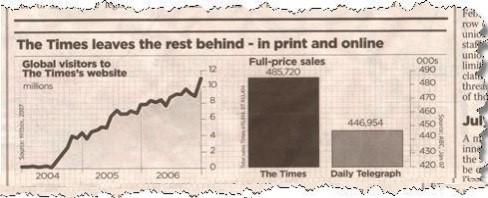
\includegraphics{figuren/MisleidingStaafdiagram_Times.jpeg}

Maar kijk eens goed naar het staafdiagram aan de rechterkant. Op het
eerste gezicht lijkt het verschil tussen de verkoopcijfers enorm omdat
de staaf van The Times een veel groter oppervlakte heeft dan die van de
Telegraph. (Die indruk wordt nog versterkt door het verschil in de
kleur!) Pas als je naar de \(y\)-as kijkt, blijkt het verschil wel mee
te vallen:

\end{example}

\begin{enumerate}
\def\labelenumi{\arabic{enumi}.}
\setcounter{enumi}{1}
\item
  \textbf{Houd ruimte tussen de staven.} Dat laat zien dat de
  categorieën van een categorische variabele niet geleidelijk in elkaar
  overlopen maar los van elkaar staan.
\item
  \textbf{Kies de volgorde van de staven verstandig.} Als de variabele
  ordinaal is, ligt het voor de hand om de natuurlijke volgorde van de
  categorieën te laten terugkomen in de volgorde van de staven. In het
  staafdiagram van de \texttt{gezondheidsstatus}
  (Figuur~\ref{fig-gezondheid-staaf}) staan de staven in de volgorde
  \emph{Slecht}, \emph{Matig}, \emph{Goed}, \emph{Zeer Goed},
  \emph{Uitstekend}. Een andere volgorde zou erg verwarrend zijn. Bij
  nominale variabelen bestaat zo'n natuurlijke volgorde niet, en hangt
  de beste volgorde af van de toepassing. Vaak is het handig om de
  staven op volgorde van grootte te sorteren, zodat de belangrijkste
  categorieën vooraan staan. Maar in andere gevallen kan bijvoorbeeld
  een alfabetische volgorde passender zijn.
\end{enumerate}

\subsection{Taart- en
stapeldiagrammen}\label{taart--en-stapeldiagrammen}

Een alternatief voor het staafdiagram is het \textbf{taartdiagram}. Een
taartdiagram representeert de verdeling van een variabele als een cirkel
-- de ``taart'' -- die verdeeld is in verschillende sectoren -- de
taartpunten. De grootte van ieder taartpunt geeft de frequentie van een
categorie aan.

\begin{example}[Burgerlijke
staat]\protect\hypertarget{exm-taart}{}\label{exm-taart}

In de NHANES dataset van het NCHS is ook van de meeste deelnemers
aangegeven wat hun burgerlijke staat is. Deze gegevens kunnen we goed
laten zien in een taartdiagram:

\begin{Shaded}
\begin{Highlighting}[]
\NormalTok{NHANES}\SpecialCharTok{$}\NormalTok{MaritalStatus }\OtherTok{\textless{}{-}} \FunctionTok{factor}\NormalTok{(}
\NormalTok{  NHANES}\SpecialCharTok{$}\NormalTok{MaritalStatus,}
  \AttributeTok{levels =} \FunctionTok{c}\NormalTok{(}\StringTok{"Married"}\NormalTok{, }\StringTok{"LivePartner"}\NormalTok{, }\StringTok{"Divorced"}\NormalTok{, }\StringTok{"Separated"}\NormalTok{, }\StringTok{"Widowed"}\NormalTok{, }\StringTok{"NeverMarried"}\NormalTok{),}
  \AttributeTok{labels =} \FunctionTok{c}\NormalTok{(}\StringTok{"Getrouwd"}\NormalTok{, }\StringTok{"Samenwonend"}\NormalTok{, }\StringTok{"Gescheiden"}\NormalTok{, }\StringTok{"Uit elkaar"}\NormalTok{, }\StringTok{"Weduwe/weduwnaar"}\NormalTok{, }\StringTok{"Nooit getrouwd"}\NormalTok{),}
  \AttributeTok{ordered =} \ConstantTok{TRUE}
\NormalTok{  )}

\NormalTok{table\_MaritalStatus }\OtherTok{\textless{}{-}} \FunctionTok{table}\NormalTok{(NHANES}\SpecialCharTok{$}\NormalTok{MaritalStatus)}

\NormalTok{data }\OtherTok{\textless{}{-}} \FunctionTok{data.frame}\NormalTok{(}
\NormalTok{  table\_MaritalStatus}
\NormalTok{)}
\FunctionTok{colnames}\NormalTok{(data) }\OtherTok{\textless{}{-}} \FunctionTok{c}\NormalTok{(}\StringTok{"BurgerlijkeStaat"}\NormalTok{, }\StringTok{"Frequentie"}\NormalTok{)}

\CommentTok{\# Taartdiagram}
\FunctionTok{ggplot}\NormalTok{(}
\NormalTok{  data, }
  \FunctionTok{aes}\NormalTok{( }
    \AttributeTok{x =} \StringTok{""}\NormalTok{, }
    \AttributeTok{y =}\NormalTok{ Frequentie, }
    \AttributeTok{fill =}\NormalTok{ BurgerlijkeStaat}
\NormalTok{    )}
\NormalTok{  ) }\SpecialCharTok{+}
  \FunctionTok{geom\_bar}\NormalTok{(}
    \AttributeTok{stat=}\StringTok{"identity"}\NormalTok{, }
    \AttributeTok{width =} \DecValTok{1}\NormalTok{, }
    \AttributeTok{color =} \StringTok{"white"}
\NormalTok{  ) }\SpecialCharTok{+}
  \FunctionTok{coord\_polar}\NormalTok{( }\StringTok{"y"}\NormalTok{, }\AttributeTok{start =} \DecValTok{0}\NormalTok{ ) }\SpecialCharTok{+}
  \FunctionTok{labs}\NormalTok{( }\AttributeTok{fill =} \StringTok{"Burgerlijke staat"}\NormalTok{) }\SpecialCharTok{+}
  \FunctionTok{theme\_void}\NormalTok{()}
\end{Highlighting}
\end{Shaded}

\begin{figure}[H]

\centering{

\includegraphics{BeschrijvendeStatistiek_files/figure-pdf/fig-taart-1.pdf}

}

\caption{\label{fig-taart}Taartdiagram van de burgerlijke staat in de
NHANES-dataset.}

\end{figure}%

Meer dan de helft van de personen in de steekproef blijkt getrouwd te
zijn.

\end{example}

Een taartdiagram maakt het vooral gemakkelijk om een beeld te krijgen
van de \emph{relatieve} frequenties van categorieën. Zo zien we
hierboven gemakkelijk dat meer dan de helft van de deelnemers aan dit
onderzoek getrouwd was. De \emph{absolute} frequenties zijn niet af te
lezen. Een taartdiagram gebruik je dus vooral als je relatieve
frequenties wilt laten zien.

Taartdiagrammen zijn alleen voor nominale variabelen aan te raden. Bij
ordinale variabelen is er altijd van nature een eerste en een laatste
categorie. Omdat een taartdiagram cirkelvormig is is er geen goede
manier om dat te laten zien. In dat geval is een \textbf{stapeldiagram}
een betere optie. Bij een stapeldiagram worden de relatieve frequenties
weergegeven als opgestapelde staven. Dit geeft wél de mogelijkheid om
dat in een specifieke volgorde te doen, zoals dat bij een ordinale
variabele wenselijk is.

\begin{example}[Stapeldiagram van
\texttt{gezondheidsstatus}]\protect\hypertarget{exm-stapel}{}\label{exm-stapel}

De variabele \texttt{gezondheidsstatus} is ordinaal; een taartdiagram is
dus niet erg geschikt om zijn verdeling weer te geven. In plaats daarvan
kan wel een stapeldiagram worden gebruikt:

\begin{Shaded}
\begin{Highlighting}[]
\NormalTok{freq\_df }\OtherTok{\textless{}{-}}\FunctionTok{data.frame}\NormalTok{(}
\NormalTok{  freq\_table}
\NormalTok{)}
\FunctionTok{colnames}\NormalTok{(freq\_df) }\OtherTok{\textless{}{-}} \FunctionTok{c}\NormalTok{(}\StringTok{"Gezondheidsstatus"}\NormalTok{, }\StringTok{"Frequentie"}\NormalTok{)}

\FunctionTok{ggplot}\NormalTok{(}
\NormalTok{  freq\_df, }
  \FunctionTok{aes}\NormalTok{( }
      \AttributeTok{x =} \StringTok{""}\NormalTok{, }
      \AttributeTok{y =}\NormalTok{ Frequentie}\SpecialCharTok{/}\FunctionTok{nrow}\NormalTok{(NHANES\_filtered), }
      \AttributeTok{fill =}\NormalTok{ Gezondheidsstatus}
\NormalTok{      )}
\NormalTok{  ) }\SpecialCharTok{+}
  \FunctionTok{geom\_bar}\NormalTok{(}
    \AttributeTok{position =} \StringTok{"stack"}\NormalTok{, }
    \AttributeTok{stat=}\StringTok{"identity"}\NormalTok{, }
    \AttributeTok{width =} \FloatTok{0.2}\NormalTok{, }
    \AttributeTok{color=}\StringTok{"black"}
\NormalTok{  ) }\SpecialCharTok{+} 
  \FunctionTok{theme\_classic}\NormalTok{() }\SpecialCharTok{+} 
  \FunctionTok{labs}\NormalTok{( }\AttributeTok{x =} \StringTok{""}\NormalTok{, }\AttributeTok{y =} \StringTok{"Relatieve frequentie"}\NormalTok{) }\SpecialCharTok{+}
  \FunctionTok{theme}\NormalTok{(}
    \AttributeTok{axis.title.x =} \FunctionTok{element\_blank}\NormalTok{(),  }\CommentTok{\# Remove x{-}axis title}
    \AttributeTok{axis.text.x =} \FunctionTok{element\_blank}\NormalTok{(),   }\CommentTok{\# Remove x{-}axis text/labels}
    \AttributeTok{axis.ticks.x =} \FunctionTok{element\_blank}\NormalTok{(),   }\CommentTok{\# Remove x{-}axis ticks}
    \AttributeTok{axis.line.x =} \FunctionTok{element\_blank}\NormalTok{()}
\NormalTok{  ) }\SpecialCharTok{+}
  \FunctionTok{scale\_y\_continuous}\NormalTok{(}\AttributeTok{limits =} \FunctionTok{c}\NormalTok{(}\DecValTok{0}\NormalTok{, }\DecValTok{1}\NormalTok{), }\AttributeTok{expand =} \FunctionTok{c}\NormalTok{(}\DecValTok{0}\NormalTok{, }\DecValTok{0}\NormalTok{))}
\end{Highlighting}
\end{Shaded}

\begin{figure}[H]

\centering{

\includegraphics{BeschrijvendeStatistiek_files/figure-pdf/fig-stapel-1.pdf}

}

\caption{\label{fig-stapel}Stapeldiagram van de variabele
Gezondheidsstatus in de NHANES-gegevens.}

\end{figure}%

\end{example}

\subsection{Histogrammen}\label{histogrammen-1}

Om de verdeling van een numerieke variabelen te laten zien wordt vaak
een \textbf{histogram} gebruikt. Een histogram lijkt op een
staafdiagram: beide zijn visualisaties van een frequentietabel waarbij
frequenties worden gerepresenteerd door de oppervlakte van staven. Het
grote verschil is dat bij numerieke gegevens de categorieën direct in
elkaar overlopen. Daarom wordt er bij een histogram geen ruimte gelaten
tussen de staven.

Net als bij staafdiagrammen is het belangrijk dat je de \(y\)-as altijd
bij 0 begint, omdat anders de oppervlaktes van de staven niet meer
proportioneel zijn met de frequenties die ze representeren.

\section{Samenhang tussen continue variabelen:
Spreidingsdiagram}\label{samenhang-tussen-continue-variabelen-spreidingsdiagram}

Om de samenhang tussen twee continue variabelen zichtbaar te maken wordt
vaak gebruik gemaakt van een spreidingsdiagram, waarbij de twee
variabelen tegen elkaar worden uitgezet.

\begin{example}[Samenhang tussen lichaamsgewicht en lengte in de
NHANES-data]\protect\hypertarget{exm-gewicht-lengte}{}\label{exm-gewicht-lengte}

In de NHANES-dataset is ook van de meeste deelnemers de lichaamslengte
gegeven. Zou er een verband zijn tussen lichaamslengte en gewicht? We
onderzoeken het met een spreidingsdiagram.

\begin{Shaded}
\begin{Highlighting}[]
\FunctionTok{ggplot}\NormalTok{(}
  \AttributeTok{data =}\NormalTok{ NHANES, }
  \FunctionTok{aes}\NormalTok{(}\AttributeTok{x =}\NormalTok{ Height, }\AttributeTok{y =}\NormalTok{ Weight)}
\NormalTok{) }\SpecialCharTok{+}
  \FunctionTok{geom\_point}\NormalTok{(}
    \AttributeTok{fill =} \StringTok{"darkorange"}\NormalTok{, }
    \AttributeTok{color =} \StringTok{"black"}
\NormalTok{  )}\SpecialCharTok{+}
  \FunctionTok{labs}\NormalTok{( }\AttributeTok{x =} \StringTok{"Gewicht (kg)"}\NormalTok{, }\AttributeTok{y =} \StringTok{"Lengte (cm)"}\NormalTok{)}
\end{Highlighting}
\end{Shaded}

\begin{figure}[H]

\centering{

\includegraphics{BeschrijvendeStatistiek_files/figure-pdf/fig-gewicht-lengte-1.pdf}

}

\caption{\label{fig-gewicht-lengte}Lichaamsgewicht uitgezet tegen lengte
in de NHANES-dataset.}

\end{figure}%

Er is duidelijk een trend te zien: langere mensen zijn gemiddeld
zwaarder. Maar er is grote variatie tussen mensen met hetzelfde gewicht,
vooral onder volwassenen.

\end{example}

\section{Samenhang tussen categorische variabelen:
mozaïekplot}\label{samenhang-tussen-categorische-variabelen-mozauxefekplot}

Hierboven hebben we het al gehad over kruistabellen. Je hebt toen gezien
dat kruistabellen worden gebruikt om verbanden te onderzoeken tussen
categorische variabelen.

Je kunt Kruistabellen visualiseren met behulp van mosaiekplots. Hoe dit
werkt, leggen we uit aan de hand van een voorbeeld.

\begin{example}[Hangt woontoestand samen met
gezondheidstoestand?]\protect\hypertarget{exm-mosaic}{}\label{exm-mosaic}

In de NHANES dataset is van iedere onderzochte persoon ook opgenomen wat
de woontoestand is. De verschillende waarden van \texttt{woontoestand}
zijn \emph{Koopwoning}, \emph{Huurwoning}, en \emph{Overig}. We vragen
ons af: is er een samenhang tussen die variabelen? Om dit te
onderzoeken, maken we eerst een kruistabel.

\begin{Shaded}
\begin{Highlighting}[]
\CommentTok{\# samenhang gezondheidstoestand en woontoestand}

\NormalTok{NHANES}\SpecialCharTok{$}\NormalTok{HomeOwn }\OtherTok{\textless{}{-}} \FunctionTok{factor}\NormalTok{(}
\NormalTok{  NHANES}\SpecialCharTok{$}\NormalTok{HomeOwn,}
  \AttributeTok{levels =} \FunctionTok{c}\NormalTok{(}\StringTok{"Other"}\NormalTok{, }\StringTok{"Rent"}\NormalTok{, }\StringTok{"Own"}\NormalTok{),}
  \AttributeTok{labels =} \FunctionTok{c}\NormalTok{(}\StringTok{"Overig"}\NormalTok{, }\StringTok{"Huurwoning"}\NormalTok{, }\StringTok{"Koopwoning"}\NormalTok{),}
  \AttributeTok{ordered =} \ConstantTok{TRUE}
\NormalTok{)}

\CommentTok{\# Generate the contingency table for HealthGen and HomeOwn}
\NormalTok{contingency\_table }\OtherTok{\textless{}{-}} \FunctionTok{table}\NormalTok{(NHANES}\SpecialCharTok{$}\NormalTok{HealthGen, NHANES}\SpecialCharTok{$}\NormalTok{HomeOwn)}
\FunctionTok{kable}\NormalTok{(}\FunctionTok{t}\NormalTok{(contingency\_table), }\AttributeTok{caption =} \StringTok{"Contingency Table of HealthGen and HomeOwn"}\NormalTok{)}
\end{Highlighting}
\end{Shaded}

\begin{longtable}[]{@{}lrrrrr@{}}
\caption{Contingency Table of HealthGen and HomeOwn}\tabularnewline
\toprule\noalign{}
& Slecht & Matig & Goed & Zeer Goed & Uitstekend \\
\midrule\noalign{}
\endfirsthead
\toprule\noalign{}
& Slecht & Matig & Goed & Zeer Goed & Uitstekend \\
\midrule\noalign{}
\endhead
\bottomrule\noalign{}
\endlastfoot
Overig & 1 & 31 & 64 & 61 & 11 \\
Huurwoning & 70 & 414 & 939 & 640 & 235 \\
Koopwoning & 114 & 556 & 1937 & 1794 & 625 \\
\end{longtable}

Deze getallen zijn lastig te overzien. Daarom maken we een mosaiekplot.

\begin{Shaded}
\begin{Highlighting}[]
\NormalTok{custom\_colors }\OtherTok{\textless{}{-}} \FunctionTok{c}\NormalTok{(}\StringTok{"skyblue"}\NormalTok{, }\StringTok{"lightgreen"}\NormalTok{, }\StringTok{"lightcoral"}\NormalTok{)}

\CommentTok{\# Create a mosaic plot using base R}
\FunctionTok{mosaicplot}\NormalTok{(}
\NormalTok{  contingency\_table, }
  \AttributeTok{col =}\NormalTok{ custom\_colors, }
  \AttributeTok{main =} \StringTok{"Samenhang tussen woontoestand en gezondheidstoestand"}\NormalTok{,}
  \AttributeTok{xlab =} \StringTok{"Gezondheidstoestand"}\NormalTok{,}
  \AttributeTok{ylab =} \StringTok{"Woontoestand"}
\NormalTok{  )}
\end{Highlighting}
\end{Shaded}

\begin{figure}[H]

\centering{

\includegraphics{BeschrijvendeStatistiek_files/figure-pdf/fig-mozaiek-1.pdf}

}

\caption{\label{fig-mozaiek}Mosaiekplot: Samenhang tussen woontoestand
en gezondheidstoestand}

\end{figure}%

\end{example}

\section{Alles samen}\label{alles-samen}

Boodschap: samenvatten met alle drie methoden. Altijd visualiseren!
Samenhang, outliers, etc.

\section{Samenvatting}\label{samenvatting}

\section{Terminologie in het Engels}\label{terminologie-in-het-engels}

\chapter{Onzekerheid in schattingen op basis van steekproeven en
experimenten}\label{onzekerheid-in-schattingen-op-basis-van-steekproeven-en-experimenten}

\addtokomafont{disposition}{\rmfamily}
\renewcommand{\ttdefault}{lcmtt}
\providecommand{\ped}[1]{_\textrm{#1}}
\providecommand{\ap}[1]{^\textrm{#1}}
\providecommand{\app}[1]{^\textrm{#1}}

\providecommand*{\angs}{\smash{\mathrm{\ring A}}}
\providecommand*{\celsius}{\mathrm{~\circ C}}
\providecommand*{\micro}{\mu}

\providecommand*{\unit}[1]{\textrm{\,#1}}

\providecommand{\E}{\mathrm{e}}
\providecommand{\I}{\mathrm{i}}
\providecommand{\sfrac}[2]{^{#1}/_{#2}}

\providecommand{\conc}[1]{\left[\mathrm{#1}\right]}

\providecommand{\command}[1]{\textsl{#1}}
\providecommand{\out}[1]{\begin{verbatim}#1\end{verbatim}}

\providecommand{\diff}{\mathrm{d}\,}

\providecommand*{\deriv}[3][]{% arguments: order of the derivative(optional), function, variable
    \frac{\diff^{#1}#2}{\diff #3^{#1}}}
\providecommand*{\pderiv}[3][]{% arguments: order of the derivative(optional), function, variable
    \frac{\partial^{#1}#2}
        {\partial #3^{#1}}}

\renewcommand{\vec}[1]{{\boldsymbol #1}}

\providecommand{\cov}[2]{\mathrm{Cov}\!\left(#1, #2\right)}
\providecommand{\var}[1]{\mathrm{Var}\!\left(#1\right)}

\providecommand{\mean}[1]{\overline{#1}}

\providecommand{\sd}[1]{\sigma\left(#1\right)}
\providecommand{\ev}[1]{\mathbb{E}\!\left(#1\right)}
\providecommand{\pr}[1]{\textrm{Pr}\!\left(#1\right)}

\providecommand{\se}[1]{\mathrm{SE}_{#1}}

\providecommand{\ct}[3]{t_{#1 (#2) #3}}

\providecommand{\HO}{H\ped{0}}
\providecommand{\HA}{H\ped{A}}
\providecommand{\df}{\mathrm{df}}

In het vorige hoofdstuk hebben we benadrukt dat biologische gegevens
onzeker zijn. Dat komt doordat gegevens vaak het resultaat zijn van
\textbf{steekproeven}, en daarnaast geplaagd worden door
\textbf{meetfouten}. Beide situaties gaan we apart bekijken. We beginnen
bij steekproeven.

\section{Belangrijke begrippen over populaties en
steekproeven}\label{belangrijke-begrippen-over-populaties-en-steekproeven}

Na iedere cursus word je gevraagd om een Caracal-enquête in te vullen.
Een belangrijk doel van die enquête is om te bepalen hoe studenten de
cursus gemiddeld beoordelen. In de praktijk vult maar een deel van de
studenten de enquête in, en dus rijst de vraag: wat kunnen we leren over
het gemiddelde oordeel van de deelnemers van een cursus op basis van een
beperkt aantal respondenten? Een vergelijkbaar probleem doet zich altijd
voor wanneer een onderzoek gebaseerd is op een \emph{steekproef}.

Laten we wat begrippen doornemen die we nodig hebben om over
steekproeven na te denken.

In veel onderzoeken zijn we geïnteresseerd in een bepaalde
\textbf{populatie}. Dat kan bijvoorbeeld de studentenpopulatie zijn, of
de populatie van Euraziatische eksters, of alle Nederlandse
diabetespatiënten.

Het onderzoek gaat vervolgens over één of meerdere \emph{variabelen}. In
deze context is een variabele een eigenschap van een individu in de
populatie, zoals bloedgroep, gewicht, of bloedsuikerwaarde na tenminste
8 uur vasten.

De waarde van een variabele verschilt meestal per individu in de
populatie. We kunnen ons daarom afvragen wat de \emph{verdeling} is van
de variabele in de populatie. De verdeling van een variabele is de
relatieve frequentie waarmee iedere mogelijke waarde in de populatie
voorkomt. Zoals je in het vorige hoofdstuk hebt gezien, kunnen we de
verdeling visualiseren, bijvoorbeeld met een staafdiagram (als variabele
categorisch is) of met een histogram (als de variabele numeriek is).

We kunnen de verdeling van een variabele ook karakteriseren met
kengetallen, zoals gemiddelde en standaardafwijking. Dit soort kenmerken
van de verdeling van een populatie worden ook wel
\textbf{populatieparameters} genoemd. Het doel van een groot gedeelte
van de onderzoeken is om een populatieparameter te bepalen. Zo kan een
onderzoek bijvoorbeeld uitzoeken wat de gemiddelde opbrengst is van
aardappelplanten waarvan een zeker gen is uitgeschakeld, of welke
fractie van de Amerikanen nu van plan is om op een bepaalde
presidentskandidaat te stemmen.

\begin{exercise}[Populatie, variabele, en
parameters]\protect\hypertarget{exr-pop-var-par}{}\label{exr-pop-var-par}

Benoem van de volgende onderzoeken de populatie, de variabele, en de
populatieparameter waarnaar onderzoek wordt gedaan. Benoem ook het type
variabele: nominaal, ordinaal, continue of discreet.

\textbf{a.} a

\textbf{b.} b

\textbf{c.} c

\textbf{d.} d

\end{exercise}

Om de populatieparameter precies te bepalen zouden we eigenlijk de
waarde van de variabele(n) moeten bepalen voor ieder individu in de
populatie. In de praktijk is dat om praktische redenen meestal
onmogelijk, omdat populaties meestal groot zijn en de onderzoeksmiddelen
beperkt. Bovendien zijn metingen vaak destructief: planten moeten worden
geoogst, proefdieren geofferd, en proefpersonen blootgesteld aan
risico's. Daarom onderzoeken we meestal slechts een aantal individuen
uit de populatie -- de steekproef. De waarden uit de steekproef
gebruiken we vervolgens om de populatieparameter te \textbf{schatten}.
Helaas betekent dat dat het resultaat niet exact is: omdat we alleen een
selectie van de populatie hebben bekeken, zal de schatting meestal
afwijken van de ware populatieparameter. Vandaar dat schattingen op
basis van steekproeven onzeker zijn.

\section{Schattingen: precisie, nauwkeurigheid, en
bias}\label{schattingen-precisie-nauwkeurigheid-en-bias}

Voordat we dieper nadenken over steekproeven is het nuttig om stil te
staan bij de verschillende manieren waarop schattingen in het algemeen
kunnen afwijken van de ware parameter.

Het is daarbij belangrijk om onderscheid te maken tussen
\textbf{precisie} en \textbf{nauwkeurigheid}. Deze begrippen worden in
Figuur~\ref{fig-precisie-vs-nauwkeurig} hieronder geïllustreerd.

\begin{figure}

\centering{

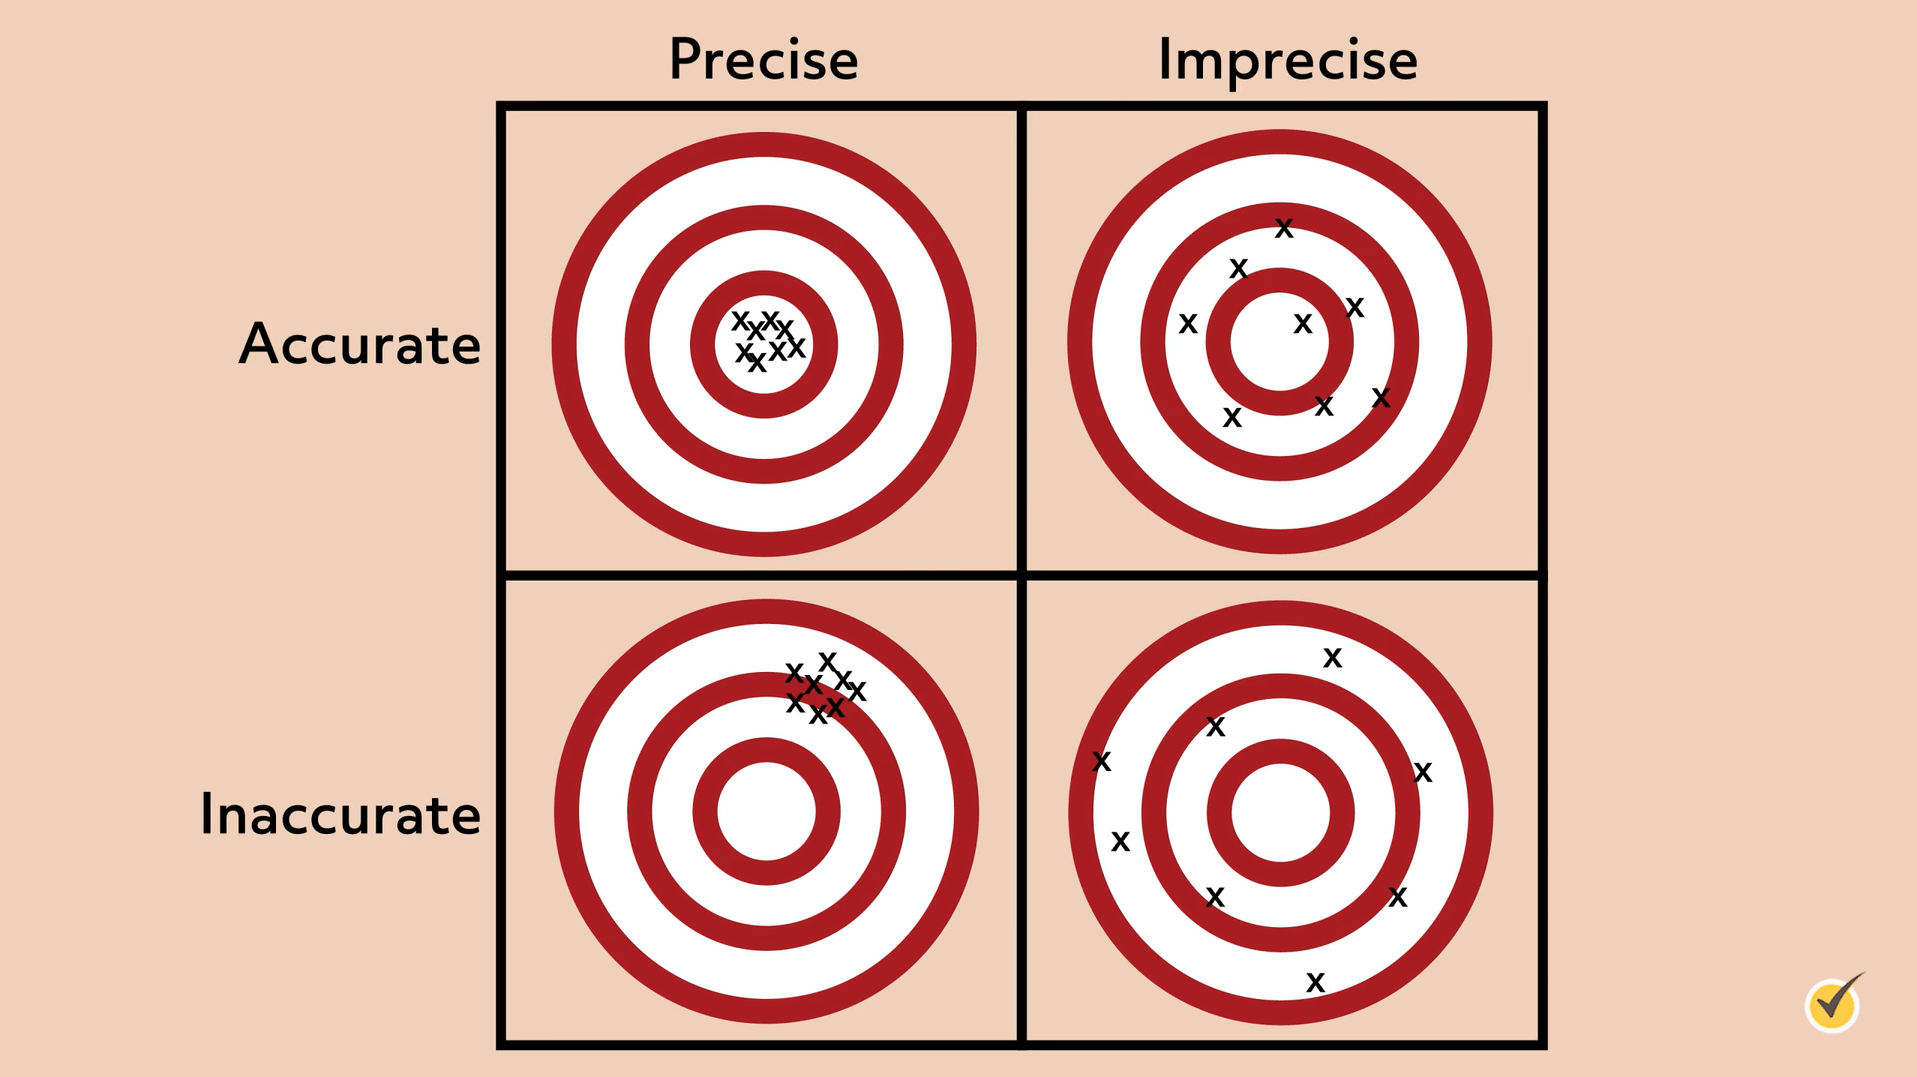
\includegraphics{figuren/Precision-Accuracy-and-Error-3.png}

}

\caption{\label{fig-precisie-vs-nauwkeurig}}

\end{figure}%

Stel je voor dat je heel vaak dezelfde methode gebruikt om een parameter
te schatten. Het resultaat kan iedere keer net iets anders uitvallen. De
methode wordt \textbf{precies} genoemd als de verschillende resultaten
weinig van elkaar verschillen. Je kunt je dat vast voorstellen: als je
's ochtends herhaaldelijk op dezelfde weegschaal gaat staan en
opeenvolgende metingen meerdere kilo's van elkaar verschillen, dan zul
je concluderen dat de weegschaal niet erg precies is.

Merk op: dat de verschillende schattingen dicht bij elkaar liggen wil
niet zeggen dat ze ook dicht bij de waarheid liggen. In beide plaatjes
in de linker-kolom van Figuur~\ref{fig-precisie-vs-nauwkeurig} is de
methode precies. Toch wijken in het onderste plaatje de waarden sterk af
van de juiste waarde (de \emph{bull's-eye}).

Een methode wordt \textbf{nauwkeurig} genoemd als het gemiddelde van de
verschillende resultaten dicht bij de waarheid ligt. In beide plaatjes
in de eerste rij van Figuur~\ref{fig-precisie-vs-nauwkeurig} zijn de
resultaten geclusterd rond de \emph{bull's-eye}. In die gevallen is de
methode dus nauwkeurig. Merk op dat een nauwkeurige methode niet precies
hoeft te zijn, zoals in het plaatje rechtsboven.

Twee verschillende aspecten dragen dus bij aan de afwijking van iedere
schatting van de juiste waarde. De eerste is er de \textbf{toevallige
fout}: wanneer dezelfde methode meerdere keren wordt gebruikt, levert
dit steeds ``toevallig'' een iets andere waarde op. Een precieze methode
geeft een kleine toevallige fout. Ten tweede is er de
\textbf{systematische fout}: de methode kan gemiddeld een te hoge of te
lage waarde opleveren. Een nauwkeurige methode geeft een kleine
systematische fout.

Als een methode een systematische fout heeft dan spreekt men ook wel
over \textbf{bias}. Bias is een Engels woord; de beste vertalingen zijn
misschien ``vertekening'' of ``vooroordeel'', maar omdat die woorden de
lading vaak niet goed dekken zullen we de Engelse term bias ook blijven
gebruiken.

Gewapend met deze begrippen keren we terug naar schattingen op basis van
steekproeven. Schattingen kunnen zowel systematische als toevallige
fouten hebben; hoe zit dat bij schattingen op basis van steekproeven?

\section{Systematische fouten in schattingen op basis van
steekproeven}\label{systematische-fouten-in-schattingen-op-basis-van-steekproeven}

Systematische fouten en bias ontstaan als individuen met bepaalde
eigenschappen een grotere kans hebben om in de steekproef terecht te
komen. Bijvoorbeeld, om de gezondheid van een populatie vogels te
onderzoeken, vang je er een aantal in netten. In dat geval zou het
kunnen dat zieke vogels zich gemakkelijker laten vangen en daarom een
grotere kans hebben om te worden opgenomen in je steekproef. Het gevolg
is dat je steekproef een vertekend beeld geeft van de populatie als
geheel. In andere woorden, de steekproef is dan niet
\textbf{representatief} voor de populatie. Dat levert systematische
fouten op, oftewel bias.

Bias kan op heel veel manieren ontstaan en is een heel belangrijk
onderwerp. Daarom komen we er later nog uitgebreid op terug.

\section{Toevallige fouten in
steekproeven}\label{toevallige-fouten-in-steekproeven}

In de aanloop naar tweedekamerverkiezingen voeren we een peiling uit. We
nemen een steekproef van 1000 Nederlandse stemgerechtigde burgers en
vragen hen op wie ze zouden stemmen als de verkiezingen vandaag zouden
plaatsvinden. Van de 1000 burgers in de steekproef zeggen er 33 van plan
te zijn om op het CDA te stemmen. We schatten dus dat het CDA op dit
moment 3,3\% van de stemmen zou krijgen.

Stel je nu voor dat we op dezelfde dag op exact dezelfde manier nóg een
steekproef zouden nemen van 1000 burgers. Zouden we dan in die tweede
steekproef weer precies 33 personen terugvinden die voor het CDA kiezen?

Dat hoeft natuurlijk niet zo te zijn. Het is best mogelijk dat we de
tweede keer toevallig maar 25 CDA-stemmers vinden, of juist 40. In dat
geval zouden we op basis van de tweede steekproef uitkomen op een
schatting van 2,5\% of juist 4.0\%. Schattingen op basis van
steekproeven worden dus geplaagd door toevallige fouten, simpelweg omdat
het resultaat afhangt van de toevallige steekproef. Omdat het woord
``toeval'\,' allerlei dingen kan betekenen hebben we het liever over
\textbf{steekproefvariabiliteit}. Steekproefvariabiliteit is het
verschijnsel dat verschillende identiek uitgevoerde steekproeven van
elkaar verschillen.

Dat steekproeven variabel zijn wil natuurlijk niet zeggen dat we
helemaal geen betrouwbare schattingen kunnen maken op basis van een
steekproef. Als in de gehele populatie 20\% van de stemgerechtigden op
het CDA wil stemmen, dan is de kans om in een steekproef van 1000
personen slechts 33 CDA-stemmers aan te treffen \emph{enorm klein}. (We
verwachten er namelijk 200.) Omgekeerd volgt daaruit: als we in onze
steekproef 3,3\% CDA-stemmers vinden dan kunnen we vrijwel uitsluiten
dat het in de gehele populatie om 20\% gaat. Later in deze cursus leer
je hoe je kunt berekenen hoe groot de onzekerheid in een schatting is.

\section{Eenvoudige aselecte
steekproeven}\label{eenvoudige-aselecte-steekproeven}

Om bias te voorkomen is het dus belangrijk om ervoor te zorgen dat je
bij het kiezen van een steekproef niet bewust of onbewust individuen met
bepaalde eigenschappen een grotere kans geeft geselecteerd te worden.
Als de manier van selecteren garandeert dat ieder individu van de
populatie, onafhankelijk van de andere leden, een gelijke kans heeft om
in de steekproef te worden opgenomen, dan levert dit een
\textbf{eenvoudige aselecte steekproef} op.

Een eenvoudige aselecte steekproef heeft verschillende voordelen. De
eerste is dat een eenvoudige aselecte steekproef geen bias heeft. Dat
maakt het mogelijk om nauwkeurige schattingen te maken. Ten tweede kun
je voor een eenvoudige aselecte steekproef vaak uitrekenen hoe groot de
toevallige fout is. Dat wil zeggen dat je de precisie van je schattingen
kunt kwantificeren. (We gaan daar in hoofstuk ?? verder op in.) Vanwege
deze voordelen gaan veel statistische analyses ervan uit dat de
steekproef eenvoudig aselect is.

In de praktijk is het vaak niet gemakkelijk om een eenvoudige aselecte
steekproef te organiseren. Als je een lijst hebt van de individuen in de
populatie, dan kan dit wel, door gebruik te maken van randomgetallen.
Ieder individu wordt dan genummerd, en we vragen een computer om uit de
lijst met nummers er willekeurig \(n\) te kiezen.

\begin{exercise}[Een aselecte
steekproef]\protect\hypertarget{exr-aselect}{}\label{exr-aselect}

Opgave: gebruik R om een eenvoudige aselecte steekproef te kiezen uit
een lijst.

\end{exercise}

In veel gevallen bestaat zo'n lijst niet, en in dat geval is de
eenvoudige aselecte steekproef vaak niet exact mogelijk. Wel kun je er
dan bij het ontwerp van je experiment naar streven om het ideaal an van
een eenvoudige aselecte steekproef zoveel mogelijk te benaderen.

Overigens maken sommige onderzoeken gebruik van meer ingewikkelder
steekproeven, zoals een \textbf{gestratificeerde steekproef}. We gaan
daar in deze cursus niet verder op in, maar als je er meer over wilt
weten kun je deze bron raadplegen: ??.

\#\# Meetfouten in experimenten

Een andere bron van onzekerheid is de \textbf{meetfout}.

\#\# Oorzaken van bias

Bespreek veel-voorkomende oorzaken van bias.

\#\# Samenvatting

\#\# Terminologie in het Engels

\chapter{Kansen en statistische
modellen}\label{kansen-en-statistische-modellen}

\addtokomafont{disposition}{\rmfamily}
\renewcommand{\ttdefault}{lcmtt}
\providecommand{\ped}[1]{_\textrm{#1}}
\providecommand{\ap}[1]{^\textrm{#1}}
\providecommand{\app}[1]{^\textrm{#1}}

\providecommand*{\angs}{\smash{\mathrm{\ring A}}}
\providecommand*{\celsius}{\mathrm{~\circ C}}
\providecommand*{\micro}{\mu}

\providecommand*{\unit}[1]{\textrm{\,#1}}

\providecommand{\E}{\mathrm{e}}
\providecommand{\I}{\mathrm{i}}
\providecommand{\sfrac}[2]{^{#1}/_{#2}}

\providecommand{\conc}[1]{\left[\mathrm{#1}\right]}

\providecommand{\command}[1]{\textsl{#1}}
\providecommand{\out}[1]{\begin{verbatim}#1\end{verbatim}}

\providecommand{\diff}{\mathrm{d}\,}

\providecommand*{\deriv}[3][]{% arguments: order of the derivative(optional), function, variable
    \frac{\diff^{#1}#2}{\diff #3^{#1}}}
\providecommand*{\pderiv}[3][]{% arguments: order of the derivative(optional), function, variable
    \frac{\partial^{#1}#2}
        {\partial #3^{#1}}}

\renewcommand{\vec}[1]{{\boldsymbol #1}}

\providecommand{\cov}[2]{\mathrm{Cov}\!\left(#1, #2\right)}
\providecommand{\var}[1]{\mathrm{Var}\!\left(#1\right)}

\providecommand{\mean}[1]{\overline{#1}}

\providecommand{\sd}[1]{\sigma\left(#1\right)}
\providecommand{\ev}[1]{\mathbb{E}\!\left(#1\right)}
\providecommand{\pr}[1]{\textrm{Pr}\!\left(#1\right)}

\providecommand{\se}[1]{\mathrm{SE}_{#1}}

\providecommand{\ct}[3]{t_{#1 (#2) #3}}

\providecommand{\HO}{H\ped{0}}
\providecommand{\HA}{H\ped{A}}
\providecommand{\df}{\mathrm{df}}

In de inleiding hebben we benadrukt dat bijna alle biologische gegevens
onzeker zijn. Soms komt dat door meetfouten, soms doordat de gegevens
schattingen zijn op basis van een steekproef. Om die gegevens te
interpreteren moeten we daarom kunnen omgaan met kansen. In dit
hoofdstuk geven we een korte introductie in kansrekenen. We beginnen met
een paar belangrijk begrippen.

\section{Basisbegrippen}\label{basisbegrippen}

Wanneer je met een gewone dobbelsteen gooit weet je van tevoren niet wat
de uitkomst zal zijn. Zo'n experiment, gebeurtenis of proces met een
onzekere uitkomst wordt een \textbf{kansexperiment} genoemd. Andere
voorbeelden zijn het willekeurig trekken van een individu uit een
populatie, of een draai aan het roulettewiel.

Een \textbf{kansvariabele} is een variabele waarvan de waarde afhangt
van de uitkomst van een kansexperiment. Een voorbeeld is het aantal ogen
van een dobbelsteen. Andere woorden voor kansvariabele zijn
\textbf{stochastische variabele} of \textbf{stochast}. Een kansvariabele
wordt meestal aangeduid met een hoofdletter, zoals \(X\).

Eerder hebben we verschillende typen variabelen besproken, zoals
continu, discreet, nominaal en ordinaal (zie
Figuur~\ref{fig-variabelen}). Kansvariabelen kunnen op dezelfde manier
worden ingedeeld.

\begin{exercise}[Typen
kansvariabelen]\protect\hypertarget{exr-type}{}\label{exr-type}

Van welk type zijn de volgende kansvariabelen?

\textbf{a.} Het aantal ogen bij het werpen van een dobbelsteen.

\textbf{b.} Het resultaat bij het gooien van een muntje (dus kop of
munt).

\end{exercise}

De verzameling van alle mogelijke uitkomsten van een kansexperiment
wordt de \textbf{kansruimte} genoemd. Bij een normale dobbelsteen is de
kansruimte de verzameling \[
    \left\{
        1, 2, 3, 4, 5, 6
    \right\}.
\]

Soms zijn we geïnteresseerd in de kans op een specifieke uitkomst. De
kans dat de uitkomst gelijk is aan 2 kunnen we noteren als
\(\textrm{Pr}\!\left(X = 2\right)\). Bij een eerlijke dobbelsteen is die
kans natuurlijk \[\textrm{Pr}\!\left(X = 2\right) =\frac{1}{6}.\]

In andere gevallen willen we weten wat de kans is op een bepaalde
\textbf{gebeurtenis}. Een gebeurtenis hoeft niet beperkt te zijn tot één
specifieke uitkomst. Bijvoorbeeld, laat \(X\) het aantal ogen zijn bij
een worp met een dobbelsteen. Dan kunnen we vragen naar de kans dat
\(X\) een oneven getal is; dat schrijf je als:
\[ \textrm{Pr}\!\left(X \textrm{ is oneven}\right). \] ``\(X\) is
oneven'' is een gebeurtenis, maar niet één specifieke uitkomst, omdat
meerdere mogelijke uitkomsten oneven zijn (namelijk 1, 3, en 5). Merk op
dat we dezelfde gebeurtenis ook zo hadden kunnen schrijven: ``\(X\) is
een element van de verzameling \(\left\{1, 3, 5\right\}\).'' Iedere
gebeurtenis is dus eigenlijk een omschrijving van een
\emph{deelverzameling} van de kansruimte.

\section{Kansen als frequenties van een lange serie identieke
kansexperimenten}\label{kansen-als-frequenties-van-een-lange-serie-identieke-kansexperimenten}

Wat is een kans nu eigenlijk precies? Deze vraag is eigenlijk veel
moeilijker dan je zou denken. Je kunt kansen op verschillende manieren
definiëren, en de aanhangers van verschillende ``kansinterpretaties''
maken hier al zeker een eeuw ruzie over. (Als dit je interesse wekt, is
\href{https://plato.stanford.edu/entries/probability-interpret/}{dit
artikel} een goede ingang tot de uitgebreide literatuur hierover.) Voor
veel berekeningen maken de definitie verschillen niet veel uit, en
daarom gebruiken we de interpretatie die in de statistiek traditioneel
het meest gebruikt wordt: de \textbf{frequentistische} interpretatie.

In de frequentistische interpretatie is de kans op een gebeurtenis
gedefiniëerd als de relatieve frequentie waarmee die gebeurtenis
voorkomt in een héél lange reeks identieke kansexperimenten. Stel dat je
steeds weer op dezelfde manier dezelfde dobbelsteen gooit. Neem even aan
dat de dobbelsteen helemaal eerlijk is. Dan zou je verwachten dat, op de
lange duur, een zesde van de uitkomsten 6 zal zijn. De relatieve
frequentie van de uitkomst 6 in een héél lange reeks identieke
kansexperimenten is dus \(\frac{1}{6}\). Daarom is de kans
\(\textrm{Pr}\!\left(X = 6\right)\) per definitie gelijk aan
\(\frac{1}{6}\).

Het lastige van deze definitie is het volgende. De definitie heeft het
over een héél lange reeks kansexperimenten. Hoe lang dan precies? Is een
miljoen keer genoeg? Of een miljard? Zolang het aantal keer dat je met
de dobbelsteen gooit eindig is, blijft het mogelijk (en zelfs
waarschijnlijk) dat de daadwerkelijke frequentie van zessen afwijkt van
\(\frac{1}{6}\). De frequentistische definitie van kansen gaat dus uit
van een reeks kansexperimenten die tot in het oneindige wordt herhaald;
alleen dan zal de frequentie van zessen met zekerheid convergeren naar
\(\frac{1}{6}\).

Een relatieve frequentie ligt altijd tussen 0 en 1 (inclusief 0 en 1).
Een kans is dus ook altijd een getal tussen 0 en 1. Als een gebeurtenis
iedere keer dat we het kansexperiment uitvoeren plaatsvindt, dan is de
kans op die gebeurtenis 1. Als een gebeurtenis nooit gebeurt, hoe vaak
we het kansexperiment ook uitvoeren, dan is de kans op die gebeurtenis
0.

Soms worden kansen in percentages uitgedrukt. Men zegt dan bijvoorbeeld
bij het gooien van een munt dat de kans op ``kop'' 50\% is. Daar is op
zich niets mis mee. Maar het heeft eigenlijk ook geen voordelen om
percentages te gebruiken, en wiskundige formules met procenten erin
worden al snel omslachtig. Wij houden het dus (net als alle wiskundigen)
zoveel mogelijk bij getallen tussen 0 en 1.

Als de kansvariabele discreet is of categorisch, dan kunnen we de kansen
van alle mogelijke uitkomsten optellen. Omdat de som van alle relatieve
frequenties altijd gelijk is aan 1 moet de som van alle kansen op alle
uitkomsten ook altijd 1 zijn.

\begin{tcolorbox}[enhanced jigsaw, arc=.35mm, bottomrule=.15mm, colframe=quarto-callout-warning-color-frame, colback=white, bottomtitle=1mm, colbacktitle=quarto-callout-warning-color!10!white, left=2mm, titlerule=0mm, coltitle=black, opacitybacktitle=0.6, breakable, toptitle=1mm, title=\textcolor{quarto-callout-warning-color}{\faExclamationTriangle}\hspace{0.5em}{Warning \ref*{wrn-continue-kansvariabelen}: De som van alle kansen bij continue kansvariabelen}, opacityback=0, toprule=.15mm, leftrule=.75mm, rightrule=.15mm]

\quartocalloutwrn{wrn-continue-kansvariabelen} 

Bij discrete en categoriale kansvariabelen is de som van de kansen op de
verschillende uitkomsten altijd gelijk aan 1. Bij continue variabelen
geldt ook zoiets, maar daar is alles wat ingewikkelder. Continue
kansvariabelen hebben oneindig veel mogelijke uitkomsten, en daardoor is
de kans op iedere mogelijke uitkomst meestal oneindig klein. Je kunt dus
niet zomaar ``alle kansen optellen''. Dat maakt dat je over continue
kansvariabelen op een speciale manier moet nadenken. We komen daar later
op terug.

\end{tcolorbox}

\section{Venn-diagrammen}\label{venn-diagrammen}

Bij het redeneren over kansen helpt het soms om de kansruimte en de
gebeurtenissen weer te geven in een zogenaamd \textbf{Venn-diagram}.

We kunnen ons de verzameling van alle mogelijke uitkomsten (de
kansruimte) voorstellen als een groot rechthoek:

\begin{Shaded}
\begin{Highlighting}[]
\FunctionTok{library}\NormalTok{(ggforce)}

\NormalTok{kleurKansruimte }\OtherTok{\textless{}{-}} \StringTok{"FloralWhite"}

\NormalTok{kansruimte }\OtherTok{\textless{}{-}} \FunctionTok{ggplot}\NormalTok{() }\SpecialCharTok{+}  
  \FunctionTok{geom\_rect}\NormalTok{(}
    \FunctionTok{aes}\NormalTok{(}\AttributeTok{xmin =} \DecValTok{0}\NormalTok{, }\AttributeTok{ymin =} \DecValTok{0}\NormalTok{, }\AttributeTok{xmax=} \DecValTok{100}\NormalTok{, }\AttributeTok{ymax =} \DecValTok{100}\NormalTok{),}
    \AttributeTok{fill =}\NormalTok{ kleurKansruimte, }\AttributeTok{color =} \StringTok{"black"}\NormalTok{, }\AttributeTok{size =}\NormalTok{ .}\DecValTok{8}
\NormalTok{    ) }\SpecialCharTok{+}
  \FunctionTok{annotate}\NormalTok{(}
    \StringTok{"text"}\NormalTok{, }
    \AttributeTok{x =} \DecValTok{2}\NormalTok{, }\AttributeTok{y =} \DecValTok{94}\NormalTok{, }
    \AttributeTok{label =} \StringTok{"kansruimte"}\NormalTok{, }
    \AttributeTok{color =} \StringTok{"black"}\NormalTok{, }
    \AttributeTok{hjust =} \DecValTok{0}\NormalTok{, }
    \AttributeTok{size =} \DecValTok{5}
\NormalTok{    ) }\SpecialCharTok{+}
  \FunctionTok{theme\_void}\NormalTok{()}

\NormalTok{kansruimte}
\end{Highlighting}
\end{Shaded}

\begin{figure}[H]

\centering{

\includegraphics{Kansrekenen_files/figure-pdf/fig-venn-1.pdf}

}

\caption{\label{fig-venn}Een minimaal Venn-diagram. Het rechthoek stelt
de volledige kansruimte voor.}

\end{figure}%

Bijvoorbeeld, bij het gooien met één dobbelsteen stelt de rechthoek de
verzameling voor van alle mogelijke uitkomsten, dus
\(\{1, 2, 3, 4, 5, 6\}\).

We zagen dat iedere gebeurtenis kan worden gerepresenteerd als een
deelverzameling van de kansruimte. We kunnen een gebeurtenis \(A\)
daarom voorsellen als een gedeelte van de kansruimte, hieronder
weergegeven als een gele cirkel:

\begin{Shaded}
\begin{Highlighting}[]
\NormalTok{kleurA }\OtherTok{\textless{}{-}} \StringTok{"Gold"}

\NormalTok{A }\OtherTok{\textless{}{-}}\NormalTok{ kansruimte }\SpecialCharTok{+}
  \FunctionTok{geom\_ellipse}\NormalTok{(}
    \FunctionTok{aes}\NormalTok{(}\AttributeTok{x0 =} \DecValTok{34}\NormalTok{, }\AttributeTok{y0 =} \DecValTok{47}\NormalTok{, }\AttributeTok{a =} \DecValTok{28}\NormalTok{,  }\AttributeTok{b =} \DecValTok{40}\NormalTok{,  }\AttributeTok{angle =} \DecValTok{0}\NormalTok{), }
    \AttributeTok{fill =}\NormalTok{ kleurA , }\AttributeTok{alpha =} \FloatTok{0.7}\NormalTok{, }\AttributeTok{size =}\NormalTok{ .}\DecValTok{8}
\NormalTok{    ) }\SpecialCharTok{+}
  \FunctionTok{annotate}\NormalTok{(}
    \StringTok{"text"}\NormalTok{, }
    \AttributeTok{x =} \DecValTok{25}\NormalTok{, }\AttributeTok{y =} \DecValTok{45}\NormalTok{, }
    \AttributeTok{label =} \FunctionTok{expression}\NormalTok{(}\FunctionTok{italic}\NormalTok{(A)), }
    \AttributeTok{color =} \StringTok{"black"}\NormalTok{, }
    \AttributeTok{hjust =} \DecValTok{0}\NormalTok{, }
    \AttributeTok{size =} \DecValTok{5}
\NormalTok{    )}

\NormalTok{A}
\end{Highlighting}
\end{Shaded}

\begin{figure}[H]

\centering{

\includegraphics{Kansrekenen_files/figure-pdf/fig-vennA-1.pdf}

}

\caption{\label{fig-vennA}Venn-diagram met gebeurtenis \(A\).}

\end{figure}%

De uitkomsten die binnen de cirkel vallen zijn de uitkomsten waarbij
gebeurtenis \(A\) plaatsvindt. De uitkomsten die buiten de cirkel vallen
zijn de uitkomsten waarbij de gebeurtenis \(A\) \emph{niet} plaatsvindt.
Bijvoorbeeld, als \(A\) de gebeurtenis is dat we een even getal gooien,
dan vinden we de uitkomsten \(\{2, 4, 6\}\) binnen de cirkel, en de
uitkomsten \(\{1, 3, 5\}\) erbuiten.

We kunnen ook meerdere gebeurtenissen weergeven in één diagram
weergeven. Hieronder zie je bijvoorbeeld een Venn-diagram met
gebeurtenissen \(A\) en \(B\):

\begin{Shaded}
\begin{Highlighting}[]
\NormalTok{kleurB }\OtherTok{\textless{}{-}} \StringTok{"DodgerBlue"}

\NormalTok{AB }\OtherTok{\textless{}{-}}\NormalTok{ A }\SpecialCharTok{+} 
  \FunctionTok{geom\_ellipse}\NormalTok{(}
    \FunctionTok{aes}\NormalTok{(}\AttributeTok{x0 =} \DecValTok{66}\NormalTok{, }\AttributeTok{y0 =} \DecValTok{47}\NormalTok{, }\AttributeTok{a =} \DecValTok{28}\NormalTok{,  }\AttributeTok{b =} \DecValTok{40}\NormalTok{,  }\AttributeTok{angle =} \DecValTok{0}\NormalTok{), }
    \AttributeTok{fill =}\NormalTok{ kleurB, }\AttributeTok{alpha =} \FloatTok{0.75}\NormalTok{, }\AttributeTok{size =}\NormalTok{ .}\DecValTok{8}
\NormalTok{    ) }\SpecialCharTok{+}
  \FunctionTok{annotate}\NormalTok{(}
    \StringTok{"text"}\NormalTok{, }
    \AttributeTok{x =} \DecValTok{75}\NormalTok{, }\AttributeTok{y =} \DecValTok{45}\NormalTok{, }
    \AttributeTok{label =} \FunctionTok{expression}\NormalTok{(}\FunctionTok{italic}\NormalTok{(B)), }
    \AttributeTok{color =} \StringTok{"black"}\NormalTok{, }
    \AttributeTok{hjust =} \DecValTok{0}\NormalTok{, }
    \AttributeTok{size =} \DecValTok{5}
\NormalTok{    )}

\NormalTok{AB}
\end{Highlighting}
\end{Shaded}

\begin{figure}[H]

\centering{

\includegraphics{Kansrekenen_files/figure-pdf/fig-vennAB-1.pdf}

}

\caption{\label{fig-vennAB}Venn-diagram met twee gebeurtenissen: \(A\)
en \(B\).}

\end{figure}%

In dit geval overlappen de twee cirkels elkaar. Dit betekent dat er
uitkomsten zijn zijn waarbij \(A\) en \(B\) allebei plaatsvinden. Een
voorbeeld zou zijn als \(A\) de gebeurtenis ``\(X\) is oneven''
voorstelt en \(B\) de gebeurtenis ``\(X\) is groter dan 3''. Die
gebeurtenissen overlappen omdat de uitkomst 5 zowel oneven is als groter
dan 3.

\section{Conditionele kansen}\label{conditionele-kansen}

Vaak verandert de kans op een gebeurtenis zodra je extra informatie
krijgt. Bijvoorbeeld, de kans dat een willekeurige gekozen persoon
zwanger is verandert zodra je leert dat deze persoon 60 jaar oud is. De
kans op gebeurtenis \(A\) \textbf{gegeven dat} gebeurtenis \(B\)
plaatsvindt, wordt geschreven als \[\textrm{Pr}\!\left(A | B\right).\]
Je spreekt dit uit als: ``de kans op \(A\) gegeven \(B\)'', of ``de kans
op \(A\) geconditioneerd op \(B\)''. In het algemeen noemen we dit
\textbf{conditionele kansen}.

Venn-diagrammen geven een nuttig perspectief op conditionele kansen.
Kijk maar eens terug naar het Venn-diagram van Figuur~\ref{fig-vennAB}.
De kans op \(A\), dus \(\textrm{Pr}\!\left(A\right)\), is de kans op
alle uitkomsten binnen de gele cirkel. Maar als gegeven is dat
gebeurtenis \(B\) plaatsvindt, dan zijn alle uitkomsten buiten de blauwe
cirkel daarmee uitgesloten. De conditionele kans
\(\textrm{Pr}\!\left(A | B\right)\) is dus de kans op de uitkomsten in
het groene gedeelte --- de overlap tussen gebeurtenissen \(A\) en \(B\)
--- relatief ten opzichte van de kans op de uitkomsten in de gehele
blauwe cirkel.

\begin{exercise}[Omdraaien van conditionele
kansen.]\protect\hypertarget{exr-omdraaien-bayes}{}\label{exr-omdraaien-bayes}

Stel dat je met een dobbelsteen gooit; \(X\) is de uitkomst van dit
kansexperiment. Gebeurtenis \(A\) is ``\(X\) is even'' en gebeurtenis
\(B\) is ``\(X < 3\)''.

\textbf{a.} Teken het Venn-diagram van Figuur~\ref{fig-vennAB} na.

\textbf{b.} Bepaal voor elke mogelijke uitkomst of deze thuishoort in
het witte, het gele, het blauwe, of het groene deel van het
Venn-diagram, en schrijf de uitkomst vervolgens in dat deel.

\textbf{c.} Wat is de kans op \(\textrm{Pr}\!\left(A|B\right)\)?

\textbf{d.} Wat is de kans \(\textrm{Pr}\!\left(B|A\right)\)?

\textbf{e} Leg uit waarom in het algemeen
\(\textrm{Pr}\!\left(A|B\right)\) niet gelijk is aan
\(\textrm{Pr}\!\left(B|A\right)\).

\end{exercise}

\section{\texorpdfstring{De kans op \(A\) en
\(B\)}{De kans op A en B}}\label{de-kans-op-a-en-b}

Vaak willen we de kans weten op een uitkomst waarbij \(A\) én \(B\)
plaatsvinden. Bijvoorbeeld: wat is de kans dat een willekeurig gekozen
persoon in Nederland diabetes heeft én hartfalen? We schrijven dit als
\[ \textrm{Pr}\!\left(A \textrm{ en } B\right). \]

Het berekenen van deze kans is erg eenvoudig als de gebeurtenissen \(A\)
en \(B\) onafhankelijk zijn. Daarom moeten we dat begrip eerst
behandelen.

\subsection{Onafhankelijke
gebeurtenissen}\label{onafhankelijke-gebeurtenissen}

Twee gebeurtenissen \(A\) en \(B\) zijn \textbf{onafhankelijk} als de
kans op gebeurtenis \(A\) niet verandert wanneer we leren dat
gebeurtenis \(B\) plaatsvindt:
\[ \textrm{Pr}\!\left(A\right) = \textrm{Pr}\!\left(A | B\right). \] In
dat geval geldt ook ook dat de kans op \(B\) niet verandert als \(A\)
gegeven wordt:
\[ \textrm{Pr}\!\left(B\right) = \textrm{Pr}\!\left(B | A\right). \]

Een voorbeeld: stel je weer voor dat we met twee eerlijke dobbelstenen
gooien--- eerst een rode, en dan een blauwe. Gebeurtenis \(A\) is dat we
met de rode dobbelsteen een zes gooien; gebeurtenis \(B\) dat we met de
blauwe dobbelsteen een zes gooien. Zijn \(A\) en \(B\) onafhankelijk?
Het is moeilijk voor te stellen dat de uitkomst van de rode dobbelsteen
effect heeft op de manier waarop de blauwe dobbelsteen rolt, en wel zo
dat het dit kans op uitkomsten van de blauwe dobbelsteen verandert.
Daarom hangt de kans dat de blauwe dobbelsteen een zes oplevert helemaal
niet af van wat er met de rode is gebeurd. Het is dus duidelijk dat
\(A\) en \(B\) onafhankelijk zijn.

Voor een tegenvoorbeeld gooien we één eerlijke dobbelsteen. Gebeurtenis
\(A\) is dat we een even aantal ogen gooien; gebeurtenis \(B\) dat we
tenminste 4 ogen gooien. Nu zijn \(A\) en \(B\) niet onafhankelijk. De
kans op \(A\) is \(\frac{1}{2}\), want er zijn net zoveel even
uitkomsten als oneven uitkomsten. Maar, als gegeven is dat \(B\)
plaatsvindt, dan sluiten we uitkomsten \(\{1, 2, 3\}\) uit en blijven
dus alleen uitkomsten \(\{4, 5, 6\}\) over. Van die drie uitkomsten zijn
er twee even, en daarom is de kans \(\textrm{Pr}\!\left(A | B\right)\)
gelijk aan \(\frac{2}{3}\). Het is duidelijk dat
\(\textrm{Pr}\!\left(A\right) \neq \textrm{Pr}\!\left(A | B\right)\), en
dus zijn \(A\) en \(B\) in dit geval niet onafhankelijk (en dus
afhankelijk).

\begin{exercise}[]\protect\hypertarget{exr-onafhankelijk}{}\label{exr-onafhankelijk}

Oefenen met onafhankelijke gebeurtenissen.

\textbf{a.} x

\textbf{b.} y

\end{exercise}

\begin{exercise}[Redeneerfout]\protect\hypertarget{exr-redeneerfout}{}\label{exr-redeneerfout}

Redeneerfout: Ik heb al 4 keer 6 gegooid dus de kans dat ik de volgende
keer wéér 6 gooi is kleiner.

\textbf{a.} x

\textbf{b.} y

\end{exercise}

\subsection{Vermenigvuldigingsregel voor onafhankelijke
gebeurtenissen}\label{vermenigvuldigingsregel-voor-onafhankelijke-gebeurtenissen}

Als \(A\) en \(B\) onafhankelijk zijn, dan kunnen we de kans op \(A\) én
\(B\) eenvoudig berekenen met de volgende
\textbf{vermenigvuldigingsregel}:
\begin{equation}\phantomsection\label{eq-vermenigvuldigingsregel}{ 
\textrm{Pr}\!\left(A \textrm{ en } B\right) = \textrm{Pr}\!\left(A\right)\textrm{Pr}\!\left(B\right).
}\end{equation} De volgende opgave laat je hopelijk inzien dat deze
regel eigenlijk heel logisch is.

\begin{exercise}[]\protect\hypertarget{exr-vermenigingsregel-intuitie}{}\label{exr-vermenigingsregel-intuitie}

Maak de vermenigvuldigingsregel intuïtief. Als 10\% van een populatie
eigenschap \(A\) heeft, en 50\% van de populatie eigenschap \(B\), en
beide eigenschappen zijn onafhankelijk, dan is de kans dat een
willekeurig gekozen persoon beide eigenschappen heeft \(0.5\times 0.1\)
(namelijk 50\% van de 10\% met eigenschap \(A\)).

\textbf{a.} a

\textbf{b.} b

\end{exercise}

\begin{exercise}[]\protect\hypertarget{exr-vermenigingsregel-intuitie}{}\label{exr-vermenigingsregel-intuitie}

Toepassen vermenigvuldigingsregel op biologische data.

\textbf{a.} a

\textbf{b.} b

\end{exercise}

\subsection{\texorpdfstring{Algemene regel voor
\(\textrm{Pr}\!\left(A \textrm{ en } B\right)\)}{Algemene regel voor \textbackslash textrm\{Pr\}\textbackslash!\textbackslash left(A \textbackslash textrm\{ en \} B\textbackslash right)}}\label{algemene-regel-voor-textrmprlefta-textrm-en-bright}

Als \(A\) en \(B\) niet onafhankelijk zijn, dan kunnen we de
vermenigvuldigingsregel niet meer gebruiken. De regel die in alle
situaties geldt is:
\begin{equation}\phantomsection\label{eq-AenBalgemeen1}{ 
\textrm{Pr}\!\left(A \textrm{ en } B\right) = \textrm{Pr}\!\left(A\right)\textrm{Pr}\!\left(B | A\right).  
}\end{equation} Om de kans op \(A\) en \(B\) te berekenen, berekenen we
dus eerst de kans op \(A\), en vermenigvuldigen die kans met de kans op
\(B\) gegeven \(A\). Omdat het niet uitmaakt welke gebeurtenis je \(A\)
noemt en welke \(B\), geldt ook:
\begin{equation}\phantomsection\label{eq-AenBalgemeen2}{
\textrm{Pr}\!\left(A \textrm{ en } B\right) = \textrm{Pr}\!\left(B\right)\textrm{Pr}\!\left(A | B\right).  
}\end{equation}\\
Je kunt dus ook de kans op \(B\) vermenigvuldigen met de kans op \(A\)
gegeven \(B\).

\begin{exercise}[]\protect\hypertarget{exr-oneindig}{}\label{exr-oneindig}

Opgave om inzichtelijk te maken dat in een oneindige rij met
experimenten de kans op \(A\) en \(B\) gelijk is aan de fractie van de
experimenten waarin \(A\) gebeurt keer de fractie \emph{van die
experimenten} waarin ook \(B\) gebeurt.

\textbf{a.} a

\textbf{b.} b

\end{exercise}

\section{\texorpdfstring{De kans op \(A\) of
\(B\)}{De kans op A of B}}\label{de-kans-op-a-of-b}

In de praktijk willen we ook vaak weten wat de kans is dat gebeurtenis
\(A\) of gebeurtenis \(B\) plaatsvindt:
\[ \textrm{Pr}\!\left(A \textrm{ of } B\right). \] Met \(A\) of \(B\)
wordt hier bedoeld dat \(A\) plaatsvindt, of \(B\) plaatsvindt, of
beiden.

Het is gemakkelijk om \(\textrm{Pr}\!\left(A \textrm{ of } B\right)\) te
berekenen als de gebeurtenissen \(A\) en \(B\) elkaar uitsluiten. Daar
moeten we het dus eerst over hebben.

\subsection{Gebeurtenissen die elkaar
uitsluiten}\label{gebeurtenissen-die-elkaar-uitsluiten}

We zeggen dat twee gebeurtenissen \(A\) en \(B\) elkaar uitsluiten als
het onmogelijk is dat \(A\) en \(B\) allebei plaatsvinden. Dat betekent
dat in het Venn-diagram de twee cirkels voor \(A\) en \(B\) niet
overlappen:

\begin{Shaded}
\begin{Highlighting}[]
\NormalTok{kansruimte }\SpecialCharTok{+} 
  \FunctionTok{geom\_ellipse}\NormalTok{(}
    \FunctionTok{aes}\NormalTok{(}\AttributeTok{x0 =} \DecValTok{28}\NormalTok{, }\AttributeTok{y0 =} \DecValTok{32}\NormalTok{, }\AttributeTok{a =} \DecValTok{25}\NormalTok{,  }\AttributeTok{b =} \DecValTok{28}\NormalTok{,  }\AttributeTok{angle =} \DecValTok{0}\NormalTok{), }
    \AttributeTok{fill =}\NormalTok{ kleurA, }\AttributeTok{alpha =} \FloatTok{0.5}\NormalTok{, }\AttributeTok{size =} \FloatTok{0.8}
\NormalTok{    ) }\SpecialCharTok{+} 
  \FunctionTok{geom\_ellipse}\NormalTok{(}
    \FunctionTok{aes}\NormalTok{(}\AttributeTok{x0 =} \DecValTok{72}\NormalTok{, }\AttributeTok{y0 =} \DecValTok{68}\NormalTok{, }\AttributeTok{a =} \DecValTok{25}\NormalTok{,  }\AttributeTok{b =} \DecValTok{28}\NormalTok{,  }\AttributeTok{angle =} \DecValTok{0}\NormalTok{), }
    \AttributeTok{fill =}\NormalTok{ kleurB, }\AttributeTok{alpha =} \FloatTok{0.5}\NormalTok{, }\AttributeTok{size =} \FloatTok{0.8}
\NormalTok{    ) }\SpecialCharTok{+}
  \FunctionTok{theme\_void}\NormalTok{() }\SpecialCharTok{+}
  \FunctionTok{annotate}\NormalTok{(}
    \StringTok{"text"}\NormalTok{, }
    \AttributeTok{x =} \DecValTok{27}\NormalTok{, }\AttributeTok{y =} \DecValTok{31}\NormalTok{, }
    \AttributeTok{label =} \FunctionTok{expression}\NormalTok{(}\FunctionTok{italic}\NormalTok{(A)), }
    \AttributeTok{color =} \StringTok{"black"}\NormalTok{, }
    \AttributeTok{hjust =} \DecValTok{0}\NormalTok{, }
    \AttributeTok{size =} \DecValTok{5}
\NormalTok{    ) }\SpecialCharTok{+}
  \FunctionTok{annotate}\NormalTok{(}
    \StringTok{"text"}\NormalTok{, }
    \AttributeTok{x =} \DecValTok{71}\NormalTok{, }\AttributeTok{y =} \DecValTok{67}\NormalTok{, }
    \AttributeTok{label =} \FunctionTok{expression}\NormalTok{(}\FunctionTok{italic}\NormalTok{(B)), }
    \AttributeTok{color =} \StringTok{"black"}\NormalTok{, }
    \AttributeTok{hjust =} \DecValTok{0}\NormalTok{, }
    \AttributeTok{size =} \DecValTok{5}
\NormalTok{    )}
\end{Highlighting}
\end{Shaded}

\begin{figure}[H]

\centering{

\includegraphics{Kansrekenen_files/figure-pdf/fig-uitsluiten-1.pdf}

}

\caption{\label{fig-uitsluiten}Venn-diagram. De gebeurtenissen \(A\) en
\(B\) sluiten elkaar uit.}

\end{figure}%

Het betekent ook dat \(\textrm{Pr}\!\left(A | B\right) = 0\) en
\(\textrm{Pr}\!\left(B | A\right) = 0\), want gegeven dat \(B\)
plaatsvindt is gebeurtenis \(A\) onmogelijk, en andersom.

\begin{exercise}[]\protect\hypertarget{exr-uitsluiten}{}\label{exr-uitsluiten}

Oefenen met gebeurtenissen die elkaar uitsluiten.

\textbf{a.} a

\textbf{b.} b

\end{exercise}

\subsection{Optelregel voor gebeurtenissen die elkaar
uitsluiten}\label{optelregel-voor-gebeurtenissen-die-elkaar-uitsluiten}

Als twee gebeurtenissen \(A\) en \(B\) elkaar uitsluiten geldt de
volgende optelregel:
\begin{equation}\phantomsection\label{eq-AofBspeciaal}{
\textrm{Pr}\!\left(A \textrm{ of } B\right)  = \textrm{Pr}\!\left(A\right) + \textrm{Pr}\!\left(B\right).
}\end{equation}

In dit geval kun je de kansen op \(A\) en \(B\) dus gewoon optellen.

\begin{exercise}[]\protect\hypertarget{exr-optelregel-1}{}\label{exr-optelregel-1}

Oefenen met optelregel.

\textbf{a.} Wat is \(\textrm{Pr}\!\left(A\right)\)?

\textbf{b.} Wat is \(\textrm{Pr}\!\left(B\right)\)?

\textbf{c.} Sluiten \(A\) en \(B\) elkaar uit?

\end{exercise}

\begin{exercise}[]\protect\hypertarget{exr-optelregel-2}{}\label{exr-optelregel-2}

\textbf{a.}

\textbf{b.}

\end{exercise}

\begin{exercise}[]\protect\hypertarget{exr-optelregel-3}{}\label{exr-optelregel-3}

\textbf{a.}

\textbf{b.}

\end{exercise}

\subsection{Algemene regel}\label{algemene-regel}

Als \(A\) en \(B\) elkaar niet uitsluiten wordt de regel iets
ingewikkelder. Maar, als je naar het Venn-diagram kijkt kun je die regel
goed begrijpen.

\begin{Shaded}
\begin{Highlighting}[]
\NormalTok{AB}
\end{Highlighting}
\end{Shaded}

\begin{figure}[H]

\centering{

\includegraphics{Kansrekenen_files/figure-pdf/fig-vennAB2-1.pdf}

}

\caption{\label{fig-vennAB2}Venn-diagram.Voor de kans op \(A\) of \(B\)
moet het groene gebied één keer worden meegeteld!}

\end{figure}%

De kans op \(A\) of \(B\) is de kans die besloten ligt in de gele en de
rode cirkel, inclusief hun overlap (het oranje gebied). Als je in dit
geval de kans op \(A\) (de kans binnen de gele cirkel) en de kans op
\(B\) (de kans binnen de rode cirkel) simpelweg zou optellen, dan zou je
de kans binnen de overlap (de oranje cirkel) dubbel meetellen. Daarom
moet je die kans er één keer vanaf trekken. Het resultaat is de volgende
algemene formule:

\begin{equation}\phantomsection\label{eq-AofBalgemeen}{ 
\textrm{Pr}\!\left(A \textrm{ of } B\right) = \textrm{Pr}\!\left(A\right) + \textrm{Pr}\!\left(B\right) - \textrm{Pr}\!\left(A \textrm{ en } B\right).
}\end{equation}

\begin{exercise}[Optelregel of algemene
regel]\protect\hypertarget{exr-algemene-regel}{}\label{exr-algemene-regel}

Stel dat \(A\) en \(B\) elkaar wederzijds uitsluiten.

\textbf{a.} Wat is \(\textrm{Pr}\!\left(A \textrm{ en } B\right)\)?

\textbf{b.} Als \(A\) en \(B\) elkaar uitsluiten mag je de optelregel
uit vergelijking\textasciitilde{}\ref{eq:AofBspeciaal} gebruiken om
\(\textrm{Pr}\!\left(A \textrm{ of } B\right)\) te berekenen. Gaat er
iets mis als je in plaats daarvan de algemene regel van
vergelijking\textasciitilde{}\ref{eq:AofBspeciaal} gebruikt?

\end{exercise}

\begin{exercise}[]\protect\hypertarget{exr-or-context}{}\label{exr-or-context}

Oefenen met \(A\) of \(B\) in biologische context

\textbf{a.} a

\textbf{b.} b

\end{exercise}

\section{Kansverdelingen}\label{kansverdelingen}

Een eerlijke dobbelsteen heeft de vorm van een bijna perfecte kubus, en
is van binnen homogeen. De symmetrische vorm maakt het vanzelfsprekend
dat alle uitkomsten even waarschijnlijk zijn. We kunnen de kansen als
volgt in een grafiek weergeven:

\begin{figure}

\centering{

Kansverdeling: kans op uitkomst 1 t/m 6 is 1/6.

}

\caption{\label{fig-uniform-die}}

\end{figure}%

Stel je nu voor dat het kansexperiment bestaat uit het werpen van niet
één maar twee dobbelstenen, zeg, een blauwe en een rode. Deze keer zijn
we geïnteresseerd in de som van het aantal ogen. De kansruimte is nu de
verzameling van getallen van 2 tot 12. Het is gemakkelijk te zien dat de
verschillende uitkomsten nu \emph{niet} meer even waarschijnlijk zijn.
Er is maar één manier om de uitkomst 2 te krijgen, namelijk als we met
zowel de rode als de blauwe dobbelsteen 1 gooien. Maar er zijn wel
\emph{zes} manieren om 7 te gooien: \(1 + 6\), \(2 + 5\), \(3 + 4\),
\(4 + 3\), \(5 + 2\), \(6 + 1\). Je zult met twee dobbelstenen dus veel
vaker 7 gooien dan 2. De kunnen de kansen weer in een grafiek weergeven:

\begin{figure}

\centering{

Kansverdeling: kansverdeling som ogen twee dobbelstenen.

}

\caption{\label{fig-kansverdeling-twee-dobbelstenen}}

\end{figure}%

In de figuur geven de oppervlaktes van de staafjes de kans weer van
iedere uitkomst.

De manier waarop de kans over de verschillende mogelijke uitkomsten
verdeeld is, wordt de \textbf{kansverdeling} genoemd. Dit begrip speelt
een grote rol in deze cursus.

\phantomsection\label{tip-kans-en-histo}
Figuur~\ref{fig-kansverdeling-twee-dobbelstenen} lijkt op een histogram.
Dat is niet voor niets. Je weet misschien nog dat we een kans op een
uitkomst hadden gedefinieerd als de frequentie van die uitkomst in een
héél lange (schier oneindige) reeks identieke kansexperimenten. Dat
betekent dat je de kansverdeling in
Figuur~\ref{fig-kansverdeling-twee-dobbelstenen} kunt interpreteren als
het histogram dat je zou krijgen als je hetzelfde kansexperiment héél
vaak zou herhalen.

\section{Kansen als oppervlakten onder de grafiek van de
kansverdeling}\label{kansen-als-oppervlakten-onder-de-grafiek-van-de-kansverdeling}

We kijken nog even terug naar de kansverdeling voor het totaal aantal
ogen bij twee dobbelstenen.

Stel dat we nu willen weten wat de kans is dat het aantal ogen groter is
dan 8 maar kleiner dan 12: \[7 < X < 11.\] Deze gebeurtenis kunnen we
ook anders uitdrukken, namelijk als
\[  X = 8 \textrm{ of } X = 9  \textrm{ of } X = 10.\] Omdat de
verschillende uitkomsten \(X = 8\), \(9\) en \(10\) elkaar uitsluiten
kunnen we de optelregel gebruiken:

\begin{equation}\phantomsection\label{eq-som8_9_10}{ \textrm{Pr}\!\left(7 < X < 11\right)  = \textrm{Pr}\!\left(X = 8\right) + \textrm{Pr}\!\left(X = 9\right) + \textrm{Pr}\!\left(X = 10\right). }\end{equation}

In de grafiek van de kansverdeling was de kans op een uitkomst
weergegeven als de oppervlakte van de bijbehorende staaf. De kans
\(\textrm{Pr}\!\left(7 < X < 11\right)\) is de som van de kansen op
uitkomsten 8, 9, en 10, en komt dus overeen met de totale oppervlakte
van de staven voor die uitkomsten. Hieronder is die oppervlakte in blauw
weergegeven:

{[}Zelfde kansverdeling, maar dan met de drie staafjes blauw
ingekleurd.{]}

In het algemeen geldt dat de kans dat de uitkomst \(X\) binnen een
bepaald interval valt, \(a < X < b\), gelijk is aan de oppervlakte onder
de grafiek van de kansverdeling dat tussen de grenzen \(a\) en \(b\) in
ligt. In dit voorbeeld was de kansvariabele numeriek en discreet, maar
we zullen zien dat ook bij continue variabelen de kans dat \(X\) in het
interval \((a, b)\) valt gegeven wordt door de oppervlakte onder de
grafiek van de kansverdeling tussen de grenzen \(a\) en \(b\).

\section{Maten voor ligging en spreiding van
kansverdelingen}\label{maten-voor-ligging-en-spreiding-van-kansverdelingen}

In hoofdstuk ?? heb je gezien dat een reeks getallen kan worden
samengevat door maten te geven voor de ligging (ook wel locatie) en
spreiding van die getallen. Op dezelfde manier kunnen we ook de
kansverdeling van een kansvariabele samenvatten door maten van ligging
en de spreiding te geven.

\subsection{Maten van ligging/locatie}\label{maten-van-ligginglocatie}

We beginnen met maten van ligging.

De \textbf{modus} van de kansverdeling van een kansvariabele \(X\) is
die uitkomst die de grootste kans heeft. Dat komt overeen met de positie
van de piek in de grafiek van de kansverdeling. Als een kansverdeling
twee pieken heeft dan wordt die ``bimodaal'' genoemd.

{[}Plaatje van een scheve verdeling (bijv. gamma-verdeling) met modus
aangegeven, en een plaatje van een bimodale verdeling{]}

Het \textbf{gemiddelde} van een kansverdeling van een kansvariabele
\(X\) wordt ook wel de \textbf{verwachtingswaarde} genoemd. Een nette
notatie daarvoor is \(\mathbb{E}\!\left(X\right)\), maar vaak wordt ook
het Griekse symbool \(\mu\) gebruikt, of \(\mu_X\) as we willen aangeven
dat het om de verwachtingswaarde van de variabele \(X\) gaat. Als de
variabele discreet is of categoriaal, dan kan de verwachtingswaarde
berekend worden als:
\[    \mathbb{E}\!\left(X\right) = \sum_x \textrm{Pr}\!\left(X = x\right) x. \]
Dat wil zeggen: we nemen het gemiddelde van alle mogelijke uitkomsten
\(x\), waarbij uitkomsten met een grotere kans zwaarder worden
meegeteld.

De \textbf{mediaan} van een kansvariabele \(\mu_\textrm{\textonehalf}\)
is de waarde zodanig dat de kans op een uitkomst kleiner dan
\(\mu_\textrm{\textonehalf}\) precies gelijk is aan \textonehalf.

{[}Scheve kansverdeling, mediaan aangegeven, kans links en rechts
aangegeven.{]}

\subsection{Maten van spreiding}\label{maten-van-spreiding}

Dan nu de maten van spreiding.

De meest gebruikte maten van spreiding zijn de variantie en de
standaardafwijking (ook vaak standaarddeviatie genoemd). De
**variantie\} van de kansverdeling van een kansvariabele \(X\) wordt
vaak genoteerd als \(\mathrm{Var}\!\left(X\right)\). Het is het
gemiddelde van de gekwadrateerde afwijking van de verwachtingswaarde:
\[ 
    \mathrm{Var}\!\left(X\right) = \mathbb{E}\!\left( \left( X - \mu \right)^2\right),
\] oftewel \[ 
    \mathrm{Var}\!\left(X\right) = \sum_x \textrm{Pr}\!\left(X = x\right) \left( x - \mu \right)^2,
\]

De standaarddeviatie is de wortel van de variantie en wordt vaak met de
Griekse letter \(\sigma\) aangeduid: \[
    \sigma = \sqrt{\mathrm{Var}\!\left(X\right)}.
\] Omgekeerd is de variantie van \(X\) dus het kwadraat van de
standaarddeviatie: \[
    \mathrm{Var}\!\left(X\right) = \sigma^2.
\] Daarom wordt de variantie van een kansvariabele ook vaak genoteerd
als \(\sigma^2\) in plaats van \(\mathrm{Var}\!\left(X\right)\).

\section{Kansen voor continue
variabelen}\label{kansen-voor-continue-variabelen}

\section{De normale verdeling}\label{de-normale-verdeling}

\section{De standaard-normale
verdeling}\label{de-standaard-normale-verdeling}

\section{Kritieke waarden van de standaard-normale
verdeling}\label{kritieke-waarden-van-de-standaard-normale-verdeling}

\section{Transformeren naar de standaard-normale
verdeling\}}\label{transformeren-naar-de-standaard-normale-verdeling}

\section{\texorpdfstring{De
\(t\)-verdeling}{De t-verdeling}}\label{de-t-verdeling}

Alvast noemen, met df.

Kritieke waarden van de \(t\)-verdeling.

\section{Optellen van meerdere
kansvariabelen}\label{optellen-van-meerdere-kansvariabelen}

We zullen in deze cursus regelmatig situaties tegenkomen waarbij we
kansvariabelen bij elkaar optellen. Bijvoorbeeld, als we met twee
dobbelstenen gooien en geïnteresseerd zijn in het totaal aantal ogen,
dan tellen we in feite twee kansvariabelen op: het aantal ogen van de
eerste dobbelsteen en het aantal ogen van de tweede dobbelsteen. Als we
die twee kansvariabelen \(X_1\) en \(X_2\) noemen, dan gaat onze
interesse dus uit naar \[ Y = X_1 + X_2.\] We hebben op deze manier een
nieuwe kansvariabele \(Y\) gedefinieerd. De vraag is nu: wat kunnen we
zeggen over de kansverdeling van \(Y\)?

Meer in het algemeen kan het zijn dat we niet twee maar \(n\)
kansvariabelen optellen. We kunnen die variabelen \(X_i\) noemen,
waarbij de index \(i\) nu een geheel getal is uit de verzameling
\(\{1, 2, \dots, n\}\). In dat algemene geval is \(Y\) dus:
\[ Y = \sum_{i=1}^n X_i.\]

\subsection{De verwachtingswaarde van een
som}\label{de-verwachtingswaarde-van-een-som}

Om te beginnen kijken we naar de verwachtingswaarde van \(Y\), dus
\(\mathbb{E}\!\left(Y\right)\). Hier is de regel heel eenvoudig: de
verwachtingswaarde van de som is de som verwachtingswaarden, dus
\begin{equation}\phantomsection\label{eq-evsom}{
\mathbb{E}\!\left(Y\right) = \sum_{i = 1}^n \mathbb{E}\!\left(X_i\right).
}\end{equation} Dit is niet erg verrassend. Zoals je weet is de
verwachtingswaarde van een variabele een ander woord voor het gemiddelde
van de kansverdeling van die variabele. Als het aantal ogen van één
dobbelsteen gemiddeld \(3 \frac{1}{2}\) is, dan is het aantal ogen van
twee dobbelstenen gemiddeld \(3 \frac{1}{2} + 3 \frac{1}{2} = 7\).

\subsection{De variantie van de som}\label{de-variantie-van-de-som}

Vervolgens bekijken we de variantie van \(Y\), dus
\(\mathrm{Var}\!\left(Y\right)\).

De berekening van de variantie van \(Y\) is gemakkelijk als de
kansvariabelen \(X_i\) allemaal \textbf{onafhankelijk\} zijn. In
paragraaf ?? hebben we al gezien wat het betekent als twee
}gebeurtenissen\} onafhankelijk zijn, maar hier hebben we het over
onafhankelijke **variabelen\}, dus we moeten nog even uitleggen wat dat
betekent.

Twee variabelen zijn onafhankelijk als de kansen op de uitkomsten van de
ene variabele niet veranderen als je de uitkomst weet van de andere
variabele. Dat is het geval als elke gebeurtenis van variabele \(X_1\)
onafhankelijk is van elke gebeurtenis van variabele \(X_2\).

\begin{exercise}[]\protect\hypertarget{exr-onafhankelijk}{}\label{exr-onafhankelijk}

Verwerkingsopgave over onafhankelijkheid.

\textbf{a.}

\textbf{b.}

\end{exercise}

Terug naar de variantie van \(Y\), waarbij \(Y\) de som was van \(n\)
kansvariabelen \(X_i\). Als alle variabelen \(X_i\) onafhankelijk zijn
van elkaar, dan is de variantie van \(Y\) simpelweg de som van de
varianties van de variabelen \(X_i\): \[
\mathrm{Var}\!\left(Y\right) = \sum_{i = 1}^n \mathrm{Var}\!\left(X_i\right).
\] \{eq-somvarianties\} Als je meerdere onafhankelijke variabelen optelt
wordt de variantie dus steeds groter.

\begin{tcolorbox}[enhanced jigsaw, arc=.35mm, bottomrule=.15mm, colframe=quarto-callout-caution-color-frame, colback=white, bottomtitle=1mm, colbacktitle=quarto-callout-caution-color!10!white, left=2mm, titlerule=0mm, coltitle=black, opacitybacktitle=0.6, breakable, toptitle=1mm, title=\textcolor{quarto-callout-caution-color}{\faFire}\hspace{0.5em}{Caution \ref*{cau-sdv-kansvariabele}: De standaarddeviatie van een som van kansvariabelen}, opacityback=0, toprule=.15mm, leftrule=.75mm, rightrule=.15mm]

\quartocalloutcau{cau-sdv-kansvariabele} 

Zoals je weet is de standaarddeviatie simpelweg de wortel van de
variantie. De standaarddeviatie van \(Y\) is in dit geval dus
\begin{equation}\phantomsection\label{eq-somvarianties}{ 
\sigma\left(Y\right) = \sqrt{\sum_{i = 1}^n \mathrm{Var}\!\left(X_i\right)}.
}\end{equation} Het is belangrijk te zien dat je eerst de varianties van
de \(X_i\) optelt en daarna pas de wortel neemt. De standaarddeviatie
van \(Y\) is dus \emph{niet} de som van de standaarddeviaties van de
\(X_i\)!

\end{tcolorbox}

\begin{exercise}[]\protect\hypertarget{exr-wortel}{}\label{exr-wortel}

Verwerkingsopgave over \(\sqrt{a + b} \neq \sqrt{a} + \sqrt{b}\).

\end{exercise}

Als de \(X_i\) niet onafhankelijk zijn, kun je niets algemeens zeggen
over de variantie van \(Y\).

\begin{exercise}[]\protect\hypertarget{exr-psychologisch-experiment}{}\label{exr-psychologisch-experiment}

Psychologisch experiment. Twee proefpersonen (mensen? zijn er
voorbeelden met primaten?). Eerste proefpersoon krijgt 10 euro (of iets
anders) maar krijgt de gelegenheid om dat bedrag te delen met de tweede
proefpersoon. \(X_1\) is het bedrag dat proefpersoon 1 zelf houdt,
\(X_2\) is het bedrag dat deze aan proefpersoon 2 geeft. Zowel \(X_1\)
als \(X_2\) zijn kansvariabelen, want verschillende proefpersonen maken
verschillende beslissingen.

\textbf{a.} Zijn \(X_1\) en \(X_2\) onafhankelijk?

\textbf{b.} Stel dat de standaarddeviatie van variabele \(X_1\) gelijk
is aan 5,€. Wat is de variantie van variabele \(X_2\)?

\textbf{c.} De variabele \(Y\) is gedefinieerd als de som van \(X_1\) en
\(X_2\), dus \(Y = X_1 + X_2\). Wat is de variantie van \(Y\)?

\textbf{d.} Zie je waarom je de varianties van \(X_1\) en \(X_2\) in dit
geval niet mag optellen?

\end{exercise}

\section{Steekproeven en experimenten zijn
kansexperimenten}\label{steekproeven-en-experimenten-zijn-kansexperimenten}

\section{Statistische modellen}\label{statistische-modellen}

\section{Samenvatting}\label{samenvatting-1}

\section{Terminologie in het Engels}\label{terminologie-in-het-engels-1}

\chapter{Het schatten van parameters}\label{het-schatten-van-parameters}

\addtokomafont{disposition}{\rmfamily}
\renewcommand{\ttdefault}{lcmtt}
\providecommand{\ped}[1]{_\textrm{#1}}
\providecommand{\ap}[1]{^\textrm{#1}}
\providecommand{\app}[1]{^\textrm{#1}}

\providecommand*{\angs}{\smash{\mathrm{\ring A}}}
\providecommand*{\celsius}{\mathrm{~\circ C}}
\providecommand*{\micro}{\mu}

\providecommand*{\unit}[1]{\textrm{\,#1}}

\providecommand{\E}{\mathrm{e}}
\providecommand{\I}{\mathrm{i}}
\providecommand{\sfrac}[2]{^{#1}/_{#2}}

\providecommand{\conc}[1]{\left[\mathrm{#1}\right]}

\providecommand{\command}[1]{\textsl{#1}}
\providecommand{\out}[1]{\begin{verbatim}#1\end{verbatim}}

\providecommand{\diff}{\mathrm{d}\,}

\providecommand*{\deriv}[3][]{% arguments: order of the derivative(optional), function, variable
    \frac{\diff^{#1}#2}{\diff #3^{#1}}}
\providecommand*{\pderiv}[3][]{% arguments: order of the derivative(optional), function, variable
    \frac{\partial^{#1}#2}
        {\partial #3^{#1}}}

\renewcommand{\vec}[1]{{\boldsymbol #1}}

\providecommand{\cov}[2]{\mathrm{Cov}\!\left(#1, #2\right)}
\providecommand{\var}[1]{\mathrm{Var}\!\left(#1\right)}

\providecommand{\mean}[1]{\overline{#1}}

\providecommand{\sd}[1]{\sigma\left(#1\right)}
\providecommand{\ev}[1]{\mathbb{E}\!\left(#1\right)}
\providecommand{\pr}[1]{\textrm{Pr}\!\left(#1\right)}

\providecommand{\se}[1]{\mathrm{SE}_{#1}}

\providecommand{\ct}[3]{t_{#1 (#2) #3}}

\providecommand{\HO}{H\ped{0}}
\providecommand{\HA}{H\ped{A}}
\providecommand{\df}{\mathrm{df}}

\section{Het doel van veel onderzoeken is het schatten van
parameters}\label{het-doel-van-veel-onderzoeken-is-het-schatten-van-parameters}

Bijna alle getallen die je leest zijn schattingen.

\section{Schattingen op basis van steekproeven zijn onzeker als gevolg
van steekproeffouten en
bias}\label{schattingen-op-basis-van-steekproeven-zijn-onzeker-als-gevolg-van-steekproeffouten-en-bias}

Box veelgemaakte fouten: Verschillende soorten bias: Sampling biases,
including: vol- unteer bias (self-selection bias), non-response /
extreme response bias, survivorship bias, ob- server bias
(vs.~blinding), recall bias, question or- der bias, acquiescence bias
self-reports

Confirmation bias

\section{Volledig onwillekeurige steekproeven elimineren
bias}\label{volledig-onwillekeurige-steekproeven-elimineren-bias}

\section{Schattingen op basis van metingen zijn onzeker door
meetfouten}\label{schattingen-op-basis-van-metingen-zijn-onzeker-door-meetfouten}

Veelgemaakte fouten: schattingen zonder maat van precisie.

\section{Het is essentieel om onzekerheid in meetfouten te
kwantificeren}\label{het-is-essentieel-om-onzekerheid-in-meetfouten-te-kwantificeren}

\section{Betrouwbaarheidsintervallen}\label{betrouwbaarheidsintervallen}

\section{Berekeningen over onzekere gegevens vereisen een
kansmodel}\label{berekeningen-over-onzekere-gegevens-vereisen-een-kansmodel}

\section{Het statistische model: Volledig willekeurige steekproeven uit
een normaal-verdeelde
variabele}\label{het-statistische-model-volledig-willekeurige-steekproeven-uit-een-normaal-verdeelde-variabele}

\(X\) normaal verdeeld

\section{De kansverdeling van het
steekproefgemiddelde}\label{de-kansverdeling-van-het-steekproefgemiddelde}

\section{De variantie van het
steekproefgemiddelde}\label{de-variantie-van-het-steekproefgemiddelde}

\section{BHI als de variantie van de populatie bekend
is}\label{bhi-als-de-variantie-van-de-populatie-bekend-is}

\(X\) is normaal verdeeld met standaarddeviatie \(\sigma\) en gemiddelde
\(\mu\). \(\mu\) is onbekend.

\(\overline{X}\) is normaal verdeeld met standaarddeviatie
\(\sigma\left(\overline{X}\right) = \sigma(X)/\sqrt{n}\).

\(Z = \frac{\overline{X} - \mu}{\sigma\left(\overline{X}\right)}\) is
standaard-normaal verdeeld.

Kritieke waarde van de standaard-normale verdeling: \[    
\textrm{Pr}\!\left(-1{,}96 < Z < 1{,}96\right) = 0{,}95.  
\] Dat betekent dat: \[    
\textrm{Pr}\!\left(-1{,}96 < \frac{\overline{X} - \mu}{\sigma\left(\overline{X}\right)} < 1{,}96\right) = 0{,}95.
\] \[    
\textrm{Pr}\!\left(-1{,}96\, \sigma\left(\overline{X}\right) < \overline{X} - \mu < 1{,}96\,\sigma\left(\overline{X}\right)\right) = 0{,}95.
\] \[
\textrm{Pr}\!\left(-\overline{X} -1{,}96\, \sigma\left(\overline{X}\right) < - \mu < - \overline{X} + 1{,}96\, \sigma\left(\overline{X}\right)\right) = 0{,}95.
\] en dus: \[
\textrm{Pr}\!\left(\overline{X} -1{,}96\, \sigma\left(\overline{X}\right) < \mu < \overline{X} + 1{,}96\, \sigma\left(\overline{X}\right)\right) = 0{,}95.
\] Dus, het 95\%-BHI is:
\[\left[\overline{X} -1{,}96\, \sigma\left(\overline{X}\right), \overline{X} + 1{,}96\, \sigma\left(\overline{X}\right) \right].\]
Andere notatie:
\[ \mu = \overline{X} \pm 1{,}96\, \sigma\left(\overline{X}\right) \]

Meestal wordt een 95\% BHI gebruikt; desgewenst kan ook een ander
percentage worden gebruikt. Dan verandert het getal \(1{,}96\) in een
ander getal, maar verder blijft de formule hetzelfde.

\section{De standaardfout van het
steekproefgemiddelde\}}\label{de-standaardfout-van-het-steekproefgemiddelde}

\[
\mathrm{SE}_{\overline{X}} = \frac{s}{\sqrt{n}}.
\]

\section{BHI als de variantie van de populatie niet bekend
is}\label{bhi-als-de-variantie-van-de-populatie-niet-bekend-is}

\(X\) is normaal verdeeld met standaarddeviatie \(\sigma\) en gemiddelde
\(\mu\). \(\mu\) en \(\sigma\) beiden onbekend.

\(\overline{X}\) is normaal verdeeld met standaarddeviatie
\(\sigma\left(\overline{X}\right) = \sigma\left(X\right)/\sqrt{n}\).
Schat \(\sigma\left(\overline{X}\right)\) met
\(\mathrm{SE}_{\overline{X}}\).

Transformatie naar \(Z\) niet mogelijk; gebruik
\(t = \frac{\overline{X} - \mu}{\mathrm{SE}_{\overline{X}}}\) volgt een
\(t\)-verdeling met \(n - 1\) vrijheidsgraden.

Kritieke waarde van de \(t\)-verdeling: \[
\textrm{Pr}\!\left( -t_{(n-1) (2) 0{,}05} < t < t_{(n-1) (2) 0{,}05} \right) = 0{,}95.
\] Dat betekent dat: \[
\textrm{Pr}\!\left(
    -t_{(n-1) (2) 0{,}05} < \frac{\overline{X} - \mu}{\mathrm{SE}_{\overline{X}}} < t_{(n-1) (2) 0{,}05} \right) = 0{,}95.
\] \[
    \textrm{Pr}\!\left(-t_{(n-1) (2) 0{,}05}\, \mathrm{SE}_{\overline{X}} < \overline{X} - \mu < t_{(n-1) (2) 0{,}05}\,\mathrm{SE}_{\overline{X}}\right) = 0{,}95.
\] \[
    \textrm{Pr}\!\left(-\overline{X} -t_{(n-1) (2) 0{,}05}\, \mathrm{SE}_{\overline{X}} < - \mu < - \overline{X} + t_{(n-1) (2) 0{,}05}\, \mathrm{SE}_{\overline{X}}\right) = 0{,}95.
\] en dus: \[
\textrm{Pr}\!\left(\overline{X} -t_{(n-1) (2) 0{,}05}\, \mathrm{SE}_{\overline{X}} < \mu < \overline{X} + t_{(n-1) (2) 0{,}05}\, \mathrm{SE}_{\overline{X}}\right) = 0{,}95.
\] Dus, het 95\%-BHI is: \[
\left[\overline{X} -t_{(n-1) (2) 0{,}05}\, \mathrm{SE}_{\overline{X}}, \overline{X} + t_{(n-1) (2) 0{,}05}\, \mathrm{SE}_{\overline{X}} \right].
\] Andere notatie: \[
    \mu = \overline{X} \pm t_{(n-1) (2) 0{,}05}\, \mathrm{SE}_{\overline{X}}.
\]

In de praktijk: bereken \(\mathrm{SE}_{\overline{X}} = s / \sqrt{n}\).

\section{Controleer of het statistische model van toepassing
is.}\label{controleer-of-het-statistische-model-van-toepassing-is.}

\begin{enumerate}
\def\labelenumi{\arabic{enumi}.}
\tightlist
\item
  Volledig willekeurige steekproef.
\item
  Normale verdeling.
\end{enumerate}

\section{Wat als het statistische model niet van toepassing
is?}\label{wat-als-het-statistische-model-niet-van-toepassing-is}

\section{Samenvatting}\label{samenvatting-2}

\section{Terminologie in het Engels}\label{terminologie-in-het-engels-2}

Standard error of the mean: SEM.

\chapter{Het toetsen van hypotheses}\label{het-toetsen-van-hypotheses}

\addtokomafont{disposition}{\rmfamily}
\renewcommand{\ttdefault}{lcmtt}
\providecommand{\ped}[1]{_\textrm{#1}}
\providecommand{\ap}[1]{^\textrm{#1}}
\providecommand{\app}[1]{^\textrm{#1}}

\providecommand*{\angs}{\smash{\mathrm{\ring A}}}
\providecommand*{\celsius}{\mathrm{~\circ C}}
\providecommand*{\micro}{\mu}

\providecommand*{\unit}[1]{\textrm{\,#1}}

\providecommand{\E}{\mathrm{e}}
\providecommand{\I}{\mathrm{i}}
\providecommand{\sfrac}[2]{^{#1}/_{#2}}

\providecommand{\conc}[1]{\left[\mathrm{#1}\right]}

\providecommand{\command}[1]{\textsl{#1}}
\providecommand{\out}[1]{\begin{verbatim}#1\end{verbatim}}

\providecommand{\diff}{\mathrm{d}\,}

\providecommand*{\deriv}[3][]{% arguments: order of the derivative(optional), function, variable
    \frac{\diff^{#1}#2}{\diff #3^{#1}}}
\providecommand*{\pderiv}[3][]{% arguments: order of the derivative(optional), function, variable
    \frac{\partial^{#1}#2}
        {\partial #3^{#1}}}

\renewcommand{\vec}[1]{{\boldsymbol #1}}

\providecommand{\cov}[2]{\mathrm{Cov}\!\left(#1, #2\right)}
\providecommand{\var}[1]{\mathrm{Var}\!\left(#1\right)}

\providecommand{\mean}[1]{\overline{#1}}

\providecommand{\sd}[1]{\sigma\left(#1\right)}
\providecommand{\ev}[1]{\mathbb{E}\!\left(#1\right)}
\providecommand{\pr}[1]{\textrm{Pr}\!\left(#1\right)}

\providecommand{\se}[1]{\mathrm{SE}_{#1}}

\providecommand{\ct}[3]{t_{#1 (#2) #3}}

\providecommand{\HO}{H\ped{0}}
\providecommand{\HA}{H\ped{A}}
\providecommand{\df}{\mathrm{df}}

\section{Rechtzaak}\label{rechtzaak}

Toeval? Of is er meer aan de hand.

In de biologie specifieker: kunnen de observaties plausibel verklaard
worden door sampling error en/of toevallige meetfouten, of is dat niet
reëel?

\section{\texorpdfstring{Hypothese
\(H_\textrm{0}\)}{Hypothese H\_\textbackslash textrm\{0\}}}\label{hypothese-h_textrm0}

\section{\texorpdfstring{Geven de gegevens aanleiding om aan
\(H_\textrm{0}\) te
twijfelen}{Geven de gegevens aanleiding om aan H\_\textbackslash textrm\{0\} te twijfelen}}\label{geven-de-gegevens-aanleiding-om-aan-h_textrm0-te-twijfelen}

Voorbeeld: steekproef uit populatie.

\section{De toetsingsgrootheid}\label{de-toetsingsgrootheid}

Voorbeeld: het gemiddelde.

\section{\texorpdfstring{De
\(P\)-waarde}{De P-waarde}}\label{de-p-waarde}

Staarten van de verdeling. Wat is de kans onder \(H_\textrm{0}\) om zo'n
extreme afwijking te krijgen, of nog extremer? Maat van verrassing: hoe
verrast zijn we door de uitkomst als we aannemen dat \(H_\textrm{0}\)
waar is? En dus ook een maat van hoeverre de gegevens bewijs vormen
tegen \(H_\textrm{0}\).

\section{De noodzaak van een statistisch
model}\label{de-noodzaak-van-een-statistisch-model}

Voorbeeld: willekeurige steekproef uit normaal-verdeelde populatie met
onbekend gemiddelde (maar bekende variantie).

Bekende variantie zeer onwaarschijnlijk.

\section{\texorpdfstring{Reflectie over
\(P\)-waarde}{Reflectie over P-waarde}}\label{reflectie-over-p-waarde}

Meest gebruikte maat van bewijs tegen \(H_\textrm{0}\), maar er is
altijd veel discussie geweest. Er bestaan alternatieven. Citeren.

\section{Hypothesetoetsen als
besluitprocedures}\label{hypothesetoetsen-als-besluitprocedures}

Vaak gebruikt en gepresenteerd als besluitprocedure.

De alternatieve hypothese \(H_\textrm{A}\). Merk op: \(H_\textrm{0}\)
meestal specifiek, \(H_\textrm{A}\) niet. De vraag is nu: kunnen we
\(H_\textrm{0}\) verwerpen?

Type-1-fout vs.~type-2-fout Kans \(\alpha\): kans op een type-1-fout
aangenomen dat \(H_\textrm{0}\) waar is.

Kans \(\beta\): kans op een type-2-fout aangenomen dat \(H_\textrm{A}\)
waar is. Die kans is niet volledig gedefinieerd omdat \(H_\textrm{A}\)
niet specifiek is. kan alleen worden berekend als een specifieke
alternatieve hypothese kiezen.

Toch: compromis.

Standaard procedure: kies een acceptabele \(\alpha\), en kies een
criterium voor verwerpen om dat te bereiken.

\section{Verwerpingsgebied}\label{verwerpingsgebied}

Verwerpen als voor gewenste \(\alpha\).

Verwerpingsgebied.

Veelvoorkomende keuze: \(\alpha = 0{,}05\). Waarom?

\section{\texorpdfstring{Relatie tussen verwerpingsgebied en
\(P\)-waarde}{Relatie tussen verwerpingsgebied en P-waarde}}\label{relatie-tussen-verwerpingsgebied-en-p-waarde}

Verwerp als \(P < \alpha\).

Statistische software zoals R geeft \(P\)-waarde. Gemakkelijk.

\section{Betrouwbaarheidsinterval}\label{betrouwbaarheidsinterval}

Geschikt voor besluitprocedure. Kwantificeert niet direct de mate van
bewijs; P-waarde wel. Aan de andere kant, geeft weer welke verzameling
van nul-hypotheses zouden worden verworpen. Geeft ook aan hoe groot de
afwijking van \(H_\textrm{0}\) waarschijnlijk is; \(P\)-waarde niet.

\section{Waarom een
besluitprocedure?}\label{waarom-een-besluitprocedure}

Standaard leerboeken vragen altijd om een conclusie: gaan we de
nul-hypothese verwerpen. Dat is eigenlijk misleidend. Het is voor een
wetenschapper meestal subtieler om te zeggen dat er een bepaalde mate
van bewijs bestaat tegen een hypothese dan om geforceerd een keuze te
maken.

In wetenschappelijke artikelen wordt zelden expliciet een nulhypothese
geformuleerd en een besluit gemaakt over het al dan niet verwerpen van
die hypothese. Over het rapporteren van statistiek hebben we het in een
later hoofdstuk uitgebreider.

\section{Anatomie van iedere
hypothesetoets}\label{anatomie-van-iedere-hypothesetoets}

\label{stap:nulhypothese}

\begin{enumerate}
\def\labelenumi{\arabic{enumi}.}
\tightlist
\item
  Stel de nul-hypothese op.
\item
  Kies een kansmodel dat past bij de casus.
\item
  Bereken een relevante toetsingsgrootheid.
\item
  Bepaald de kansverdeling van de toetsingsgrootheid onder de
  nulhypothese, op basis van het kansmodel.
\item
  Bereken de \(P\)-waarde.
\item
  Trek je conclusies.
\end{enumerate}

In de laatste stap trek je je conclusies over \(H_\textrm{0}\) op basis
van de \(P\)-waarde. Hoe kleiner \(P\) is, hoe opmerkelijker de gevonden
toetsingsgrootheid is onder de nulhypothese, en hoe meer je de
nulhypothese dus in twijfel zult trekken. Vaak wordt de waarde
\(0{,}05\) als grens gehanteerd: als \(P < 0{,}05\), dan spreekt men van
een ``statistisch significant'\,' resultaat. Merk op dat een
\(P\)-waarde van \(0{,}05\) onder de nulhypothese gemiddeld één op de 20
keer voorkomt (want \(0{,}05\) is precies een twintigste). Dat wil
zeggen dat de toetsingsgrootheid zeker opmerkelijk is onder
\(H_\textrm{0}\), maar zeker niet ondenkbaar. Een waarde \(P = 0{,}05\)
is dus maar matig bewijs tegen de nulhypothese.

Als je per sé een besluit wil nemen over het al-dan-niet verwerpen van
de nulhypothese, dan zul je in stap 1 ook moeten besluiten welke
\(\alpha\) (kans op een type-I fout) je acceptabel vindt. In stap 6
bepaal je dan of \(P < \alpha\). Als dat zo is, dan verwerp je de
nulhypothese. Meestal wordt in de praktijk de waarde \(\alpha = 0{,}05\)
als grens genomen; je verwerpt in dat geval de nulhypothese als
\(P < 0{,}05\).

\section{Box veelgemaakte fouten:}\label{box-veelgemaakte-fouten}

Reasoning based on small sample sizes (incl.~\(n = 1\))

\section{Samenvatting}\label{samenvatting-3}

\section{Terminologie in het Engels}\label{terminologie-in-het-engels-3}

\bookmarksetup{startatroot}

\chapter*{References}\label{references}
\addcontentsline{toc}{chapter}{References}

\markboth{References}{References}

\phantomsection\label{refs}
\begin{CSLReferences}{0}{1}
\end{CSLReferences}

\cleardoublepage
\phantomsection
\addcontentsline{toc}{part}{Bijlagen}
\appendix

\chapter{Het gemiddelde minimaliseert de
kwadratensom}\label{sec-kwadratensom}

\addtokomafont{disposition}{\rmfamily}
\renewcommand{\ttdefault}{lcmtt}
\providecommand{\ped}[1]{_\textrm{#1}}
\providecommand{\ap}[1]{^\textrm{#1}}
\providecommand{\app}[1]{^\textrm{#1}}

\providecommand*{\angs}{\smash{\mathrm{\ring A}}}
\providecommand*{\celsius}{\mathrm{~\circ C}}
\providecommand*{\micro}{\mu}

\providecommand*{\unit}[1]{\textrm{\,#1}}

\providecommand{\E}{\mathrm{e}}
\providecommand{\I}{\mathrm{i}}
\providecommand{\sfrac}[2]{^{#1}/_{#2}}

\providecommand{\conc}[1]{\left[\mathrm{#1}\right]}

\providecommand{\command}[1]{\textsl{#1}}
\providecommand{\out}[1]{\begin{verbatim}#1\end{verbatim}}

\providecommand{\diff}{\mathrm{d}\,}

\providecommand*{\deriv}[3][]{% arguments: order of the derivative(optional), function, variable
    \frac{\diff^{#1}#2}{\diff #3^{#1}}}
\providecommand*{\pderiv}[3][]{% arguments: order of the derivative(optional), function, variable
    \frac{\partial^{#1}#2}
        {\partial #3^{#1}}}

\renewcommand{\vec}[1]{{\boldsymbol #1}}

\providecommand{\cov}[2]{\mathrm{Cov}\!\left(#1, #2\right)}
\providecommand{\var}[1]{\mathrm{Var}\!\left(#1\right)}

\providecommand{\mean}[1]{\overline{#1}}

\providecommand{\sd}[1]{\sigma\left(#1\right)}
\providecommand{\ev}[1]{\mathbb{E}\!\left(#1\right)}
\providecommand{\pr}[1]{\textrm{Pr}\!\left(#1\right)}

\providecommand{\se}[1]{\mathrm{SE}_{#1}}

\providecommand{\ct}[3]{t_{#1 (#2) #3}}

\providecommand{\HO}{H\ped{0}}
\providecommand{\HA}{H\ped{A}}
\providecommand{\df}{\mathrm{df}}

We willen aantonen dat het gemiddelde van een reeks getallen \(x_i\) de
kwadratensom minimaliseert. De kwadratensom rond een willekeurig waarde
\(m\) wordt gedefinieerd als:

\[
\mathrm{SS}(m) = \sum_i \left(x_i - m\right)^2.
\]

De vraag is nu: wat is de waarde van \(m\) die deze som zo klein
mogelijk maakt?

Om het minimum te vinden, stellen we de afgeleide van \(\mathrm{SS}(m)\)
naar \(m\) gelijk aan nul. De afgeleide van \(\mathrm{SS}(m)\) naar
\(m\) is:

\[
% arguments: order of the derivative(optional), function, variable
    \frac{\mathrm{d}\,^{}\mathrm{SS}(m)}{\mathrm{d}\,m^{}} = -2 \sum_{i=1}^n \left( x_i - m\right).
\] (We hebben hiervoor de kettingregel gebruikt.) We herschrijven dit
naar:

\[
% arguments: order of the derivative(optional), function, variable
    \frac{\mathrm{d}\,^{}\mathrm{SS}(m)}{\mathrm{d}\,m^{}} = 2 \sum_{i=1}^n (m - x_i).
\]

We stellen deze afgeleide gelijk aan nul om minimum te vinden:

\[
2 \sum_{i=1}^n (m - x_i) = 0.
\] De factor 2 kunnen we wegstrepen. De vergelijking zegt dus eigenlijk
dat de som van alle afwijkingen van \(m\) gelijk aan nul moet zijn.

Merk op dat \(\sum_{i=1}^n m = n m\), omdat je \(n\) keer de waarde
\(m\) optelt. We kunnen de vergelijking hierboven dus uitwerken tot: \[
n m - \sum_{i=1}^n x_i = 0,
\] Oplossen naar \(m\) geeft:

\[
m = \frac{\sum_i x_i}{n} = \overline{x}.
\]

Met andere woorden, de waarde van \(m\) die de kwadratensom
minimaliseert, is het gemiddelde van de reeks getallen, oftewel
\(\overline{x}\). Dit laat zien dat het gemiddelde precies de waarde is
die de kwadratensom minimaliseert.


\backmatter


\end{document}
